\chapter{基本使用}

\section{定义信息}
我们在开始排版之间,需要导言区定义一些个人的信息来填充封面,也就是在 \verb|\begin{document}| 之前,插入以下代码:
\begin{lstlisting}[caption=个人信息定义]
\information{
  classification=中图分类号,     
  studentno=学号,       
  degree=学历,          
  title=论文 \titlesep 题目,         
  name=姓名,           
  mentor=导师,     
  mentorrank=导师职称,     
  major=专业,           
  research=研究方向,     
  institute=学院,       
  year=年,           
  month=月,        
  day=日,           
  keywordscn=关键词1\keysepcn 关键词2\keysepcn 关键词3,     
  keywordsen=KeyWord1\keysepen KeyWord2\keysepen KeyWord3
}
\end{lstlisting}
这样,我们就初步完成了封面信息的填充,注意,\verb|\titlesep| 只能用于标题的换行,且只能用一次,一般标题长度足够了,\verb|\keysepcn| 和 \verb|\keysepen| 分别用于中英文关键词的分隔。

\section{正文编写}
如果排版时只在一个文件内,则修改时会十分不便,建议使用多文件排版,然后通过 \verb|\include{file}| 引入。正文和致谢的引入位置在参考文献之前,这点需要注意,正确的位置如下所示:
\begin{lstlisting}[caption=正文引入]
  % 正文开始
  \mainmatter
  
  % 具体正文章节
  \chapter{基本使用}

\section{定义信息}
我们在开始排版之间,需要导言区定义一些个人的信息来填充封面,也就是在 \verb|\begin{document}| 之前,插入以下代码:
\begin{lstlisting}[caption=个人信息定义]
\information{
  classification=中图分类号,     
  studentno=学号,       
  degree=学历,          
  title=论文 \titlesep 题目,         
  name=姓名,           
  mentor=导师,     
  mentorrank=导师职称,     
  major=专业,           
  research=研究方向,     
  institute=学院,       
  year=年,           
  month=月,        
  day=日,           
  keywordscn=关键词1\keysepcn 关键词2\keysepcn 关键词3,     
  keywordsen=KeyWord1\keysepen KeyWord2\keysepen KeyWord3
}
\end{lstlisting}
这样,我们就初步完成了封面信息的填充,注意,\verb|\titlesep| 只能用于标题的换行,且只能用一次,一般标题长度足够了,\verb|\keysepcn| 和 \verb|\keysepen| 分别用于中英文关键词的分隔。

\section{正文编写}
如果排版时只在一个文件内,则修改时会十分不便,建议使用多文件排版,然后通过 \verb|\include{file}| 引入。正文和致谢的引入位置在参考文献之前,这点需要注意,正确的位置如下所示:
\begin{lstlisting}[caption=正文引入]
  % 正文开始
  \mainmatter
  
  % 具体正文章节
  \chapter{基本使用}

\section{定义信息}
我们在开始排版之间,需要导言区定义一些个人的信息来填充封面,也就是在 \verb|\begin{document}| 之前,插入以下代码:
\begin{lstlisting}[caption=个人信息定义]
\information{
  classification=中图分类号,     
  studentno=学号,       
  degree=学历,          
  title=论文 \titlesep 题目,         
  name=姓名,           
  mentor=导师,     
  mentorrank=导师职称,     
  major=专业,           
  research=研究方向,     
  institute=学院,       
  year=年,           
  month=月,        
  day=日,           
  keywordscn=关键词1\keysepcn 关键词2\keysepcn 关键词3,     
  keywordsen=KeyWord1\keysepen KeyWord2\keysepen KeyWord3
}
\end{lstlisting}
这样,我们就初步完成了封面信息的填充,注意,\verb|\titlesep| 只能用于标题的换行,且只能用一次,一般标题长度足够了,\verb|\keysepcn| 和 \verb|\keysepen| 分别用于中英文关键词的分隔。

\section{正文编写}
如果排版时只在一个文件内,则修改时会十分不便,建议使用多文件排版,然后通过 \verb|\include{file}| 引入。正文和致谢的引入位置在参考文献之前,这点需要注意,正确的位置如下所示:
\begin{lstlisting}[caption=正文引入]
  % 正文开始
  \mainmatter
  
  % 具体正文章节
  \chapter{基本使用}

\section{定义信息}
我们在开始排版之间,需要导言区定义一些个人的信息来填充封面,也就是在 \verb|\begin{document}| 之前,插入以下代码:
\begin{lstlisting}[caption=个人信息定义]
\information{
  classification=中图分类号,     
  studentno=学号,       
  degree=学历,          
  title=论文 \titlesep 题目,         
  name=姓名,           
  mentor=导师,     
  mentorrank=导师职称,     
  major=专业,           
  research=研究方向,     
  institute=学院,       
  year=年,           
  month=月,        
  day=日,           
  keywordscn=关键词1\keysepcn 关键词2\keysepcn 关键词3,     
  keywordsen=KeyWord1\keysepen KeyWord2\keysepen KeyWord3
}
\end{lstlisting}
这样,我们就初步完成了封面信息的填充,注意,\verb|\titlesep| 只能用于标题的换行,且只能用一次,一般标题长度足够了,\verb|\keysepcn| 和 \verb|\keysepen| 分别用于中英文关键词的分隔。

\section{正文编写}
如果排版时只在一个文件内,则修改时会十分不便,建议使用多文件排版,然后通过 \verb|\include{file}| 引入。正文和致谢的引入位置在参考文献之前,这点需要注意,正确的位置如下所示:
\begin{lstlisting}[caption=正文引入]
  % 正文开始
  \mainmatter
  
  % 具体正文章节
  \include{chapters/chapter1}
  \include{chapters/chapter2}
  \include{chapters/chapter3}
  \include{chapters/chapter4}
  \include{chapters/chapter5}
  \include{chapters/chapter6}
  \include{chapters/chapter7}
  
  % 致谢
  \include{chapters/thanks}
  
  % 参考文献开始
  \addreference
\end{lstlisting}
在正文内部,可以分四个层级,例如:
\begin{lstlisting}[caption=章节命令使用]
  \chapter{一级标题}
  \section{二级标题}
  \subsection{三级标题}
  \subsubsection{四级标题}
\end{lstlisting}
\begin{figure}[H]
  \centering 
  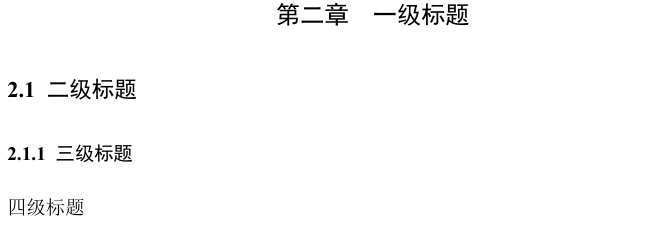
\includegraphics[width=0.5 \linewidth]{figures/2-1}
  \caption{标题格式}
  \label{2:1}
\end{figure}
\section{常用命令}
\subsection{分页}
分页包裹连续分页和奇数页分页,分别对应命令 \verb|\clearpage| 和 \verb|\cleardoublepage|,其中,\verb|\clearpage| 在空白页不会显示页眉页脚
\subsection{文本装饰}
\begin{lstlisting}[caption=文本装饰]
  \CJKunderdot{汉字,下加点} \\
  \CJKunderline{汉字,下划线} \\
  \CJKunderdblline{汉字,双下划线} \\
  \CJKunderwave{汉字,下波浪线} \\
  \CJKsout{汉字,删除线} \\
  \CJKxout{汉字,删除线}
\end{lstlisting}
\begin{center}
  \fbox{
    \parbox{8em}{
      \CJKunderdot{汉字,下加点} \\
      \CJKunderline{汉字,下划线} \\
      \CJKunderdblline{汉字,双下划线} \\
      \CJKunderwave{汉字,下波浪线} \\
      \CJKsout{汉字,删除线} \\
      \CJKxout{汉字,删除线}
    }
  }
\end{center}

\subsection{列表环境}
\LaTeX 提供了三种列表环境:编号的 enumerate 环境,不编号的 itemize 环境和使用关键字的 description 环境。在列表环境内部使用 \verb|\item| 命令开始一个列表项,他可以带一个可选参数表示手动编号或关键字。

enumerate 环境使用数字自动编号:
\clearpage
\begin{lstlisting}[caption=enumerate环境]
  \begin{enumerate}
    \item 中文
    \item English
    \item 日本語
  \end{enumerate}
\end{lstlisting}

\begin{center}
  \fbox{
    \parbox{8em}{
      \begin{enumerate}
        \item 中文
        \item English
        \item 日本語
      \end{enumerate}
    }
  }
\end{center}
itemize 环境不编号,但会在每个条目前加一个符号以示标记:
\begin{lstlisting}[caption=enumerate环境]
  \begin{itemize}
    \item 中文
    \item English
    \item 日本語
  \end{itemize}
\end{lstlisting}

\begin{center}
  \fbox{
    \parbox{8em}{
      \begin{itemize}
        \item 中文
        \item English
        \item 日本語
      \end{itemize}
    }
  }
\end{center}
description 环境总是使用 \verb|\item| 命令的可选参数,把它作为条目关键字加粗显示:
\clearpage
\begin{lstlisting}[caption=enumerate环境]
    \begin{description}
        \item[中文] 中国的语言文学 
        \item[English] The language of England
        \item[日本語] 日本の言語
    \end{description}
\end{lstlisting}

\begin{center}
  \fbox{
    \parbox{14em}{
      \begin{description}
        \item[中文] 中国的语言文学 
        \item[English] The language of England
        \item[日本語] 日本の言語
      \end{description}
    }
  }
\end{center}
这几个环境可以嵌套使用(至多四层),\LaTeX 会自动处理不同层次的缩进和编号。
  \chapter{参考文献}

\section{参考文件格式}
目前本模板仅有 ~{\color{blue}{GB/T~7714-2005}}~和~{\color{blue}{GB/T~7714-2015}}~样式,默认采用~{\color{blue}{GB/T~7714-2015}}~样式,如果需要使用其他格式,请自行寻找或编写 \emph{.bst}文件。

\section{BibTeX 的使用}
模板中有一个\emph{reference.bib}文件,是存放参考文献信息的数据库,通过谷歌学术、微软学术或是百度学术,查找文献时,把其 BibTeX 的引用信息复制到这个文件里,在你需要引用的地方,按照如下方式引用:
\begin{lstlisting}[caption=BibTeX 引用参考文献]
  \cite{bibid}  % bibid 就是你复制引文信息的第一个参数
  \cite{bibid1,bibid2,bibid2}  % 同时引用多个文献
\end{lstlisting}
  

\chapter{数学排版}
\section{行内和行间公式}
数学公式有两种排版方式:其一是与文字混排,称为\textbf{行内公式};其二是单独列为一行排版,称为行间公式。 

行内公式由一对 \texttt\$ 符号包裹:
\begin{lstlisting}
  $a^2 + b^2 = c^2$
\end{lstlisting}
\begin{center}
  \fbox{
    \parbox{10em}{
      \centering $a^2 + b^2 = c^2$
    }
  }
\end{center}
单独成行的行间公式在 \LaTeX{} 里由 equation 环境包裹。equation 环境为公式自动生成一个编号,这个编号可以用 \verb|\label| 和 \verb|\ref| 生成交叉引用,
amsmath 的 \verb|\eqref| 命令甚至为引用自动加上圆括号;还可以用 \verb|\tag| 命令手动修改公式的编号,或者用 \verb|\notag| 命令取消为公式编号。
\begin{lstlisting}[caption=多行公式示例一]
    The Pythagorean theorem is:
    \begin{equation}
      a^2 + b^2 = c^2 \label{pythagorean}
    \end{equation}
    Equation \eqref{pythagorean} is called `Gougu theorem' in Chinese.
\end{lstlisting}
\begin{center}
  \fbox{
    \parbox{30em}{
      The Pythagorean theorem is:
      \begin{equation}
      a^2 + b^2 = c^2 \label{pythagorean}
      \end{equation}
      Equation \eqref{pythagorean} is
      called `Gougu theorem' in Chinese.
    }
  }
\end{center}
\clearpage
\begin{lstlisting}[caption=多行公式示例二]
  It's wrong to say
  \begin{equation}
    1 + 1 = 3 \tag{dumb}
  \end{equation}
  or
  \begin{equation}
    1 + 1 = 4 \notag
  \end{equation}
\end{lstlisting}
\begin{center}
	\fbox{
		\parbox{30em}{
		    It's wrong to say
			\begin{equation}
			1 + 1 = 3 \tag{dumb}
			\end{equation}
			or
			\begin{equation}
			1 + 1 = 4 \notag
			\end{equation}
		}
	}
\end{center}

如果需要直接使用不带编号的行间公式,则将公式用命令 \verb|\[| 和 \verb|\]| 包裹,与之等效的是 \verb|displaymath| 环境。有的人更喜欢 \verb|equation|$*$ 环境,体现了带星号和不带星号的环境之间的区别。

\begin{lstlisting}[caption=多行公式示例三]
  \begin{equation*}
    a^2 + b^2 = c^2
  \end{equation*}
  For short:
  \[ a^2 + b^2 = c^2 \]
  Or if you like the long one:
  \begin{displaymath}
    a^2 + b^2 = c^2
  \end{displaymath}
\end{lstlisting}
\clearpage
\begin{center}
	\fbox{
		\parbox{30em}{
			\begin{equation*}
			a^2 + b^2 = c^2
			\end{equation*}
			For short:
			\[ a^2 + b^2 = c^2 \]
			Or if you like the long one:
			\begin{displaymath}
			a^2 + b^2 = c^2
			\end{displaymath}
		}
	}
\end{center}

我们通过一个例子展示行内公式和行间公式的对比。为了与文字相适应,行内公式在排版大的公式元素(分式、巨算符等)时显得很“局促”:
\begin{lstlisting}[caption=综合示例]
  In text:
  $\lim_{n \to \infty} \sum_{k=1}^n \frac{1}{k^2} = \frac{\pi^2}{6}$.
  In display:
  \[
    \lim_{n \to \infty}
    \sum_{k=1}^n \frac{1}{k^2}
    = \frac{\pi^2}{6}
  \]
\end{lstlisting}
\begin{center}
	\fbox{
		\parbox{30em}{
			In text:
			$\lim_{n \to \infty} \sum_{k=1}^n \frac{1}{k^2} = \frac{\pi^2}{6}$.
			
			In display:
			\[
			  \lim_{n \to \infty}
			  \sum_{k=1}^n \frac{1}{k^2}
			  = \frac{\pi^2}{6}
			\]
		}
	}
\end{center}
\clearpage
\section{数学模式}
当用户使用 \$ 开启行内公式输入,或是使用 \verb|\[| 命令、equation 环境时,\LaTeX{} 就进入了数学模式。数学模式相比于文本模式有以下特点:
\begin{enumerate}
	\item 数学模式中输入的空格被忽略。数学符号的间距默认由符号的性质(关系符号、运算符等)决定。
	需要人为引入间距时,使用 \verb|\quad| 和 \verb|\qquad| 等命令。
	\item 不允许有空行(分段)。行间公式中也无法用 \verb|\\| 命令手动换行。排版多行公式需要用到其他公式环境。
	\item 所有的字母被当作数学公式中的变量处理,字母间距与文本模式不一致,也无法生成单词之间的空格。
\end{enumerate}
\section{数学符号}
\subsection{一般符号}
\begin{table}[htp]
	\centering
	\caption{希腊字母} 
	\begin{quote}\footnotesize%
		\verb|\Alpha|,\verb|\Beta| 等希腊字母符号不存在,因为它们和拉丁字母 A,B 等一模一样;
		小写字母里也不存在 \verb|\omicron|,直接用拉丁字母 $o$ 代替。
	\end{quote}
	\begin{symbols}{*4{cl}}
		\hline
		\SYM{\alpha}     & \SYM{\theta}     & \SYM{o}          & \SYM{\upsilon}  \\
		\SYM{\beta}      & \SYM{\vartheta}  & \SYM{\pi}        & \SYM{\phi}      \\
		\SYM{\gamma}     & \SYM{\iota}      & \SYM{\varpi}     & \SYM{\varphi}   \\
		\SYM{\delta}     & \SYM{\kappa}     & \SYM{\rho}       & \SYM{\chi}      \\
		\SYM{\epsilon}   & \SYM{\lambda}    & \SYM{\varrho}    & \SYM{\psi}      \\
		\SYM{\varepsilon}& \SYM{\mu}        & \SYM{\sigma}     & \SYM{\omega}    \\
		\SYM{\zeta}      & \SYM{\nu}        & \SYM{\varsigma}  &                 \\
		\SYM{\eta}       & \SYM{\xi}        & \SYM{\tau}       &                 \\[1ex]
		\SYM{\Gamma}     & \SYM{\Lambda}    & \SYM{\Sigma}     & \SYM{\Psi}      \\
		\SYM{\Delta}     & \SYM{\Xi}        & \SYM{\Upsilon}   & \SYM{\Omega}    \\
		\SYM{\Theta}     & \SYM{\Pi}        & \SYM{\Phi}       &                 \\[1ex]
		\AMSM{\varGamma} & \AMSM{\varLambda}& \AMSM{\varSigma}  & \AMSM{\varPsi}      \\
		\AMSM{\varDelta} & \AMSM{\varXi}    & \AMSM{\varUpsilon}& \AMSM{\varOmega}    \\
		\AMSM{\varTheta} & \AMSM{\varPi}    & \AMSM{\varPhi}    &                 \\
		\hline
	\end{symbols}
\end{table}
\clearpage
~\\
\begin{table}[H]
	\centering
	\caption{其他符号}
	\begin{symbols}{*4{cl}}
		\hline
		\SYM{\dots}       & \SYM{\cdots}      & \SYM{\vdots}      & \SYM{\ddots}     \\
		\SYM{\hbar}       & \SYM{\imath}      & \SYM{\jmath}      & \SYM{\ell}       \\
		\SYM{\Re}         & \SYM{\Im}         & \SYM{\aleph}      & \SYM{\wp}        \\
		\SYM{\forall}     & \SYM{\exists}     & \LSYM{\mho}       & \SYM{\partial}   \\
		\SYM{'}           & \SYM{\prime}      & \SYM{\emptyset}   & \SYM{\infty}     \\
		\SYM{\nabla}      & \SYM{\triangle}   & \LSYM{\Box}       & \LSYM{\Diamond}  \\
		\SYM{\bot}        & \SYM{\top}        & \SYM{\angle}      & \SYM{\surd}      \\
		\SYM{\diamondsuit} & \SYM{\heartsuit} & \SYM{\clubsuit}   & \SYM{\spadesuit} \\
		\SYM{\neg} or \verb|\lnot| & \SYM{\flat} & \SYM{\natural}    & \SYM{\sharp}     \\
		\hline
	\end{symbols}
\end{table}

\subsection{指数、上下标和导数}
在\LaTeX{}中一般用 $\^$ 和 $\_$ 标明上下标,如果上下标不是一个字符需要使用花括号包裹,否则只对上下标符号后第一个字符起作用。

导数符号 \texttt' (${}'$) 是一类特殊的上标,可以适当连用表示多阶导数,也可以在其后连用上标:
\begin{lstlisting}
  $f(x) = x^2 \quad f'(x) = 2x \quad f''^{2}(x) = 4$
\end{lstlisting}
\begin{center}
	\fbox{
		\parbox{20em}{
			\centering $f(x) = x^2 \quad f'(x) = 2x \quad f''^{2}(x) = 4$
		}
	}
\end{center}
\subsection{分式和根式}
分式使用 \verb|\frac|\{分子\}\{分母\} 来书写。分式的大小在行间公式中是正常大小,而在行内被极度压缩。
\begin{center}
	\fbox{
		\parbox{20em}{
			In display style:
			\[
			3/8 \qquad \frac{3}{8}
			\qquad \tfrac{3}{8}
			\]
			In text style:
			$1\frac{1}{2}$~hours \qquad
			$1\dfrac{1}{2}$~hours
		}
	}
\end{center}
一般的根式使用 \verb|\sqrt{...}|;表示 $n$ 次方根时写成 \verb|\sqrt[n]{...}|.
\begin{center}
	\fbox{
		\parbox{20em}{
			\centering
			$\sqrt{x} \Leftrightarrow x^{1/2}
			\quad \sqrt[3]{2}
			\quad \sqrt{x^{2} + \sqrt{y}}$
		}
	}
\end{center}
特殊的分式形式,如二项式结构,由 amsmath 宏包的 \verb|\binom| 命令生成:
\begin{lstlisting}
  Pascal's rule is
  \[
    \binom{n}{k} =\binom{n-1}{k} + \binom{n-1}{k-1}
  \]
\end{lstlisting}
\begin{center}
	\fbox{
		\parbox{20em}{
			Pascal's rule is
			\[
			\binom{n}{k} =\binom{n-1}{k} + \binom{n-1}{k-1}
			\]
		}
	}
\end{center}
\subsection{关系符}
\LaTeX{}常见的关系符号如下表所示,同时还提供了自定义二元关系符的命令 \verb|\stackrel|,用于将一个符号代价在原有的二元关系符之上:
\begin{lstlisting}
  \[
    f_n(x) \stackrel{*}{\approx} 1
  \]
\end{lstlisting}
\begin{center}
	\fbox{
		\parbox{20em}{
			\centering
			\[
			  f_n(x) \stackrel{*}{\approx} 1
			\]
		}
	}
\end{center}
\clearpage
~\\
\begin{table}[H]
	\centering
	\caption{二元关系符}
	\begin{quote}\footnotesize%
		所有的二元关系符都可以加 \verb|\not| 前缀得到相反意义的关系符,例如 \verb|\not=| 就得到不等号(同 \verb|\ne|)。
	\end{quote}
	\begin{symbols}{*3{cl}}
		\hline
		\SYM{<}              & \SYM{>}                    & \SYM{=}          \\
		\SYM{\leq} or \verb|\le|   & \SYM{\geq} or \verb|\ge| & \SYM{\equiv}     \\
		\SYM{\ll}            & \SYM{\gg}                  & \SYM{\doteq}     \\
		\SYM{\prec}          & \SYM{\succ}                & \SYM{\sim}       \\
		\SYM{\preceq}        & \SYM{\succeq}              & \SYM{\simeq}     \\
		\SYM{\subset}        & \SYM{\supset}              & \SYM{\approx}    \\
		\SYM{\subseteq}      & \SYM{\supseteq}            & \SYM{\cong}      \\
		\LSYM{\sqsubset}     & \LSYM{\sqsupset}           & \LSYM{\Join}     \\
		\SYM{\sqsubseteq}    & \SYM{\sqsupseteq}          & \SYM{\bowtie}    \\
		\SYM{\in}            & \SYM{\ni}, \verb|\owns|      & \SYM{\propto}    \\
		\SYM{\vdash}         & \SYM{\dashv}               & \SYM{\models}    \\
		\SYM{\mid}           & \SYM{\parallel}            & \SYM{\perp}      \\
		\SYM{\smile}         & \SYM{\frown}               & \SYM{\asymp}     \\
		\SYM{:}              & \SYM{\notin}               & \SYM{\neq} or \verb|\ne| \\
		\hline
	\end{symbols}
\end{table}

\begin{table}[H]
	\centering
	\caption{\AmS{} 二元关系符} 
	\begin{symbols}{*3{cl}}
		\hline
		\AMSSYM{\lessdot}           & \AMSSYM{\gtrdot}            & \AMSSYM{\doteqdot} \\
		\AMSSYM{\leqslant}          & \AMSSYM{\geqslant}          & \AMSSYM{\risingdotseq}     \\
		\AMSSYM{\eqslantless}       & \AMSSYM{\eqslantgtr}        & \AMSSYM{\fallingdotseq}    \\
		\AMSSYM{\leqq}              & \AMSSYM{\geqq}              & \AMSSYM{\eqcirc}           \\
		\AMSSYM{\lll} or \verb|\llless| & \AMSSYM{\ggg}               & \AMSSYM{\circeq}  \\
		\AMSSYM{\lesssim}           & \AMSSYM{\gtrsim}            & \AMSSYM{\triangleq}        \\
		\AMSSYM{\lessapprox}        & \AMSSYM{\gtrapprox}         & \AMSSYM{\bumpeq}           \\
		\AMSSYM{\lessgtr}           & \AMSSYM{\gtrless}           & \AMSSYM{\Bumpeq}           \\
		\AMSSYM{\lesseqgtr}         & \AMSSYM{\gtreqless}         & \AMSSYM{\thicksim}         \\
		\AMSSYM{\lesseqqgtr}        & \AMSSYM{\gtreqqless}        & \AMSSYM{\thickapprox}      \\
		\AMSSYM{\preccurlyeq}       & \AMSSYM{\succcurlyeq}       & \AMSSYM{\approxeq}         \\
		\AMSSYM{\curlyeqprec}       & \AMSSYM{\curlyeqsucc}       & \AMSSYM{\backsim}          \\
		\AMSSYM{\precsim}           & \AMSSYM{\succsim}           & \AMSSYM{\backsimeq}        \\
		\AMSSYM{\precapprox}        & \AMSSYM{\succapprox}        & \AMSSYM{\vDash}            \\
		\AMSSYM{\subseteqq}         & \AMSSYM{\supseteqq}         & \AMSSYM{\Vdash}            \\
		\AMSSYM{\shortparallel}     & \AMSSYM{\Supset}            & \AMSSYM{\Vvdash}           \\
		\AMSSYM{\blacktriangleleft} & \AMSSYM{\sqsupset}          & \AMSSYM{\backepsilon}      \\
		\AMSSYM{\vartriangleright}  & \AMSSYM{\because}           & \AMSSYM{\varpropto}        \\
		\AMSSYM{\blacktriangleright}& \AMSSYM{\Subset}            & \AMSSYM{\between}          \\
		\AMSSYM{\trianglerighteq}   & \AMSSYM{\smallfrown}        & \AMSSYM{\pitchfork}        \\
		\AMSSYM{\vartriangleleft}   & \AMSSYM{\shortmid}          & \AMSSYM{\smallsmile}       \\
		\AMSSYM{\trianglelefteq}    & \AMSSYM{\therefore}         & \AMSSYM{\sqsubset}         \\
		\hline
	\end{symbols}
\end{table}
\subsection{算符}
\begin{table}[htp]
	\centering
	\caption{二元运算符}
	\begin{symbols}{*3{cl}}
		\hline
		\SYM{+}              & \SYM{-}              &                     \\
		\SYM{\pm}            & \SYM{\mp}            & \SYM{\triangleleft} \\
		\SYM{\cdot}          & \SYM{\div}           & \SYM{\triangleright}\\
		\SYM{\times}         & \SYM{\setminus}      & \SYM{\star}         \\
		\SYM{\cup}           & \SYM{\cap}           & \SYM{\ast}          \\
		\SYM{\sqcup}         & \SYM{\sqcap}         & \SYM{\circ}         \\
		\SYM{\vee}, \verb|\lor| & \SYM{\wedge},\verb|\land|  & \SYM{\bullet}   \\
		\SYM{\oplus}         & \SYM{\ominus}        & \SYM{\diamond}      \\
		\SYM{\odot}          & \SYM{\oslash}        & \SYM{\uplus}        \\
		\SYM{\otimes}        & \SYM{\bigcirc}       & \SYM{\amalg}        \\
		\SYM{\bigtriangleup} &\SYM{\bigtriangledown}& \SYM{\dagger}       \\
		\LSYM{\lhd}          & \LSYM{\rhd}          & \SYM{\ddagger}      \\
		\LSYM{\unlhd}        & \LSYM{\unrhd}        & \SYM{\wr}           \\
		\hline
	\end{symbols}
\end{table}
\begin{table}[htp]
	\centering
	\caption{\hologo{AmS} 二元运算符} 
	\begin{symbols}{*3{cl}}
		\hline
		\AMSSYM{\dotplus}        & \AMSSYM{\centerdot}      &       \\
		\AMSSYM{\ltimes}         & \AMSSYM{\rtimes}         & \AMSSYM{\divideontimes} \\
		\AMSSYM{\doublecup}      & \AMSSYM{\doublecap}      & \AMSSYM{\smallsetminus} \\
		\AMSSYM{\veebar}         & \AMSSYM{\barwedge}       & \AMSSYM{\doublebarwedge}\\
		\AMSSYM{\boxplus}        & \AMSSYM{\boxminus}       & \AMSSYM{\circleddash}   \\
		\AMSSYM{\boxtimes}       & \AMSSYM{\boxdot}         & \AMSSYM{\circledcirc}   \\
		\AMSSYM{\intercal}       & \AMSSYM{\circledast}     & \AMSSYM{\rightthreetimes} \\
		\AMSSYM{\curlyvee}       & \AMSSYM{\curlywedge}     & \AMSSYM{\leftthreetimes} \\
		\hline
	\end{symbols}
\end{table}
$\nabla$(\verb|\nabla|) 和 $\partial$(\verb|\partial|) 也是常用的算符,虽然它们不属于二元算符。
\LaTeX{} 将数学函数的名称作为一个算符排版,字体为直立字体。
\vspace{2em}
\begin{table}[htp]
	\centering
	\caption{\LaTeX{} 作为算符的函数名称一览}
	\begin{tabular}{*{5}{p{5em}}}
		\hline
		\multicolumn{5}{c}{\textbf{不带上下限的算符}} \\
		\hline
		\verb|\sin| & \verb|\arcsin| & \verb|\sinh| & \verb|\exp| & \verb|\dim| \\
		\verb|\cos| & \verb|\arccos| & \verb|\cosh| & \verb|\log| & \verb|\ker| \\
		\verb|\tan| & \verb|\arctan| & \verb|\tanh| & \verb|\lg|  & \verb|\hom| \\
		\verb|\cot| & \verb|\arg|    & \verb|\coth| & \verb|\ln|  & \verb|\deg| \\
		\verb|\sec| & \verb|\csc|    & \\
		\hline
		\multicolumn{5}{c}{\textbf{带上下限的算符}} \\
		\hline
		\verb|\lim| & \verb|\limsup| & \verb|\liminf| & \verb|\sup| & \verb|\inf| \\
		\verb|\min| & \verb|\max|    & \verb|\det|    & \verb|\Pr|  & \verb|\gcd| \\
		\hline
	\end{tabular}
\end{table}
\clearpage
\begin{lstlisting}
  \[
    \lim_{x \rightarrow 0}
    \frac{\sin x}{x}=1
  \]
\end{lstlisting}
\begin{center}
	\fbox{
		\parbox{20em}{
			\centering
		    \[
			  \lim_{x \rightarrow 0}
			  \frac{\sin x}{x}=1
			\]
		}
	}
\end{center}
对于求模表达式,\LaTeX{} 提供了 \verb|\bmod| 和 \verb|\pmod| 命令,前者相当于一个二元运算符,后者作为同余表达式的后缀:
\begin{lstlisting}
  $a\bmod b \\
  x\equiv a \pmod{b}$
\end{lstlisting}
\begin{center}
	\fbox{
		\parbox{20em}{
		  $a\bmod b \\
		  x\equiv a \pmod{b}$
		}
	}
\end{center}
amsmath 还允许用户在导言区用 \verb|\DeclareMathOperator|定义自己的算符,其中带星号的命令定义带上下限的算符:
\begin{verbatim}
\DeclareMathOperator{\argh}{argh}
\DeclareMathOperator*{\nut}{Nut}
\end{verbatim}
\begin{lstlisting}
  \[\argh 3 = \nut_{x=1} 4x\]
\end{lstlisting}
\begin{center}
	\fbox{
		\parbox{20em}{
			\[\argh 3 = \nut_{x=1} 4x\]
		}
	}
\end{center}
\subsection{巨算符}
积分号 $\int$(\verb|\int|)、求和号 $\sum$ (\verb|\sum|) 等符号称为\textbf{巨算符}。巨算符在行内公式和行间公式的大小和形状有区别。
\begin{lstlisting}
  In text:
  $\sum_{i=1}^n \quad
  \int_0^{\frac{\pi}{2}} \quad
  \oint_0^{\frac{\pi}{2}} \quad
  \prod_\epsilon $ \\
  In display:
  \[\sum_{i=1}^n \quad
  \int_0^{\frac{\pi}{2}} \quad
  \oint_0^{\frac{\pi}{2}} \quad
  \prod_\epsilon \]
\end{lstlisting}
\begin{center}
	\fbox{
		\parbox{20em}{
			In text:
			$\sum_{i=1}^n \quad
			\int_0^{\frac{\pi}{2}} \quad
			\oint_0^{\frac{\pi}{2}} \quad
			\prod_\epsilon $ \\
			In display:
			\[\sum_{i=1}^n \quad
			\int_0^{\frac{\pi}{2}} \quad
			\oint_0^{\frac{\pi}{2}} \quad
			\prod_\epsilon \]
		}
	}
\end{center}
巨算符的上下标位置可由 \verb|\limits| 和 \verb|\nolimits| 调整,前者令巨算符类似 $\lim$ 或求和算符 $\sum$,上下标位于上下方;后者令巨算符类似积分号,上下标位于右上方和右下方。

\begin{lstlisting}
  In text:
  $\sum\limits_{i=1}^n \quad
  \int\limits_0^{\frac{\pi}{2}} \quad
  \prod\limits_\epsilon $ \\
  In display:
  \[\sum\nolimits_{i=1}^n \quad
  \int\limits_0^{\frac{\pi}{2}} \quad
  \prod\nolimits_\epsilon \]
\end{lstlisting}
\begin{center}
	\fbox{
		\parbox{20em}{
			In text:
			$\sum\limits_{i=1}^n \quad
			\int\limits_0^{\frac{\pi}{2}} \quad
			\prod\limits_\epsilon $ \\
			In display:
			\[\sum\nolimits_{i=1}^n \quad
			\int\limits_0^{\frac{\pi}{2}} \quad
			\prod\nolimits_\epsilon \]
		}
	}
\end{center}
amsmath 宏包还提供了 \verb|\substack|,能够在下限位置书写多行表达式;subarray
环境更进一步,令多行表达式可选择居中 (c) 或左对齐 (l):
\begin{lstlisting}
  \[
  \sum_{\substack{0\le i\le n \\
  j\in \mathbb{R}}}
  P(i,j) = Q(n)
  \]
  \[
  \sum_{\begin{subarray}{l}
  0\le i\le n \\
  j\in \mathbb{R}
  \end{subarray}}
  P(i,j) = Q(n)
  \]
\end{lstlisting}
\begin{center}
	\fbox{
		\parbox{20em}{
			\[
			\sum_{\substack{0\le i\le n \\
					j\in \mathbb{R}}}
			P(i,j) = Q(n)
			\]
			\[
			\sum_{\begin{subarray}{l}
				0\le i\le n \\
				j\in \mathbb{R}
				\end{subarray}}
			P(i,j) = Q(n)
			\]
		}
	}
\end{center}
\clearpage
~\\
\begin{table}[H]
	\centering
	\caption{巨算符}
	\def\arraystretch{2.2}
	\begin{symbols}{*3{ccl}}
		\hline
		\BIGSYM{\sum}      & \BIGSYM{\bigcup}   & \BIGSYM{\bigvee}  \\
		\BIGSYM{\prod}     & \BIGSYM{\bigcap}   & \BIGSYM{\bigwedge} \\
		\BIGSYM{\coprod}   & \BIGSYM{\bigsqcup} & \BIGSYM{\biguplus} \\
		\BIGSYM{\int}      & \BIGSYM{\oint}     & \BIGSYM{\bigodot} \\
		\BIGSYM{\bigoplus} & \BIGSYM{\bigotimes} & \\
		\AMSBIG{\iint}     & \AMSBIG{\iiint}    & \AMSBIG{\iiiint}  \\
		\AMSBIG{\idotsint} &                    & \\
		\hline
	\end{symbols}
\end{table}
\subsection{数学重音和上下括号}
\begin{table}[htp]
	\centering
	\caption{数学重音符号}
	\begin{quote}\footnotesize%
		最后一个 \verb|\wideparen| 依赖 yhmath 宏包。
	\end{quote}
	\begin{symbols}{*3{cl}}
		\hline
		\ACC{\hat}{a}   & \ACC{\check}{a} & \ACC{\tilde}{a}       \\
		\ACC{\acute}{a} & \ACC{\grave}{a} & \ACC{\breve}{a}       \\
		\ACC{\bar}{a}   & \ACC{\vec}{a}   & \ACC{\mathring}{a}    \\
		\ACC{\dot}{a}   & \ACC{\ddot}{a}  & \AMSACC{\dddot}{a}    \\
		\AMSACC{\ddddot}{a} \\[1ex]
		\ACC{\widehat}{AAA} & \ACC{\widetilde}{AAA} & \ACC{\wideparen}{AAA} \\
		\hline
	\end{symbols}
\end{table}

\begin{table}[htp]
	\centering
	\caption{作为重音的箭头符号} 
	\begin{symbols}{*2{cl}}
		\hline
		\ACC{\overrightarrow}{AB}     & \AMSACC{\underrightarrow}{AB}     \\
		\ACC{\overleftarrow}{AB}      & \AMSACC{\underleftarrow}{AB}      \\
		\AMSACC{\overleftrightarrow}{AB} & \AMSACC{\underleftrightarrow}{AB} \\
		\hline
	\end{symbols}
\end{table}

\cmd{overbrace} 和 \cmd{underbrace} 命令用来生成上/下括号,各自可带一个上/下标公式。
\begin{lstlisting}
  $\underbrace{\overbrace{(a+b+c)}^6
  \cdot \overbrace{(d+e+f)}^7}
  _\text{meaning of life} = 42$
\end{lstlisting}

\begin{center}
	\fbox{
		\parbox{20em}{
			\centering
			$\underbrace{\overbrace{(a+b+c)}^6
				\cdot \overbrace{(d+e+f)}^7}
			_\text{meaning of life} = 42$
		}
	}
\end{center}

\subsection{箭头}
常用的箭头包括 \cmd{rightarrow} ($\rightarrow$,或 \cmd{to})、\cmd{leftarrow}($\leftarrow$,或 \cmd{gets})等。
\begin{table}[H]
	\centering
	\caption{箭头}
	\begin{symbols}{*2{cl}}
		\hline
		\SYM{\leftarrow} or \cmd{gets} & \SYM{\longleftarrow} \\
		\SYM{\rightarrow} or \cmd{to}   & \SYM{\longrightarrow} \\
		\SYM{\leftrightarrow}    & \SYM{\longleftrightarrow} \\
		\SYM{\Leftarrow}         & \SYM{\Longleftarrow}     \\
		\SYM{\Rightarrow}        & \SYM{\Longrightarrow}    \\
		\SYM{\Leftrightarrow}    & \SYM{\Longleftrightarrow}\\
		\SYM{\mapsto}            & \SYM{\longmapsto}        \\
		\SYM{\hookleftarrow}     & \SYM{\hookrightarrow}    \\
		\SYM{\leftharpoonup}     & \SYM{\rightharpoonup}    \\
		\SYM{\leftharpoondown}   & \SYM{\rightharpoondown}  \\
		\SYM{\rightleftharpoons} & \SYM{\iff}               \\
		\SYM{\uparrow}           & \SYM{\downarrow} \\
		\SYM{\updownarrow}       & \SYM{\Uparrow} \\
		\SYM{\Downarrow}         & \SYM{\Updownarrow} \\
		\SYM{\nearrow}           & \SYM{\searrow} \\
		\SYM{\swarrow}           & \SYM{\nwarrow} \\
		\LSYM{\leadsto}          &              \\
		\hline
	\end{symbols}
\end{table}
amsmath 的 \cmd{xleft\-arrow} 和 \cmd{xright\-arrow} 命令提供了长度可以伸展的箭头,并且可以为箭头增加上下标:
\begin{lstlisting}
  \[ a\xleftarrow{x+y+z} b \]
  \[ c\xrightarrow[x<y]{a*b*c}d \]
\end{lstlisting}
\begin{center}
	\fbox{
		\parbox{20em}{
			 \[ a\xleftarrow{x+y+z} b \]
			\[ c\xrightarrow[x<y]{a*b*c}d \]
		}
	}
\end{center}

\subsection{括号和定界符}

\begin{table}[htp]
	\centering
	\caption{定界符}
	\begin{quote}\footnotesize%
		amsmath 还定义了 \cmd{lvert}、\cmd{rvert} 和 \cmd{lVert}、\cmd{rVert},
		分别作为 \cmd{vert} 和 \cmd{Vert} 对应的开符号(左侧)和闭符号(右侧)的命令。
	\end{quote}
	\begin{symbols}{*4{cl}}
		\hline
		\SYM{(}                  & \SYM{)}                  & \SYM{\uparrow}     & \SYM{\downarrow}   \\
		\SYM{[}  or \cmd{lbrack} & \SYM{]}  or \cmd{rbrack} & \SYM{\Uparrow}     & \SYM{\Downarrow}   \\
		\SYM{\{} or \cmd{lbrace} & \SYM{\}} or \cmd{rbrace} & \SYM{\updownarrow} & \SYM{\Updownarrow} \\
		\SYM{|}  or \cmd{vert}   & \SYM{\|} or \cmd{Vert}   & \SYM{\lceil}       & \SYM{\rceil}       \\
		\SYM{\langle}            & \SYM{\rangle}            & \SYM{\lfloor}      & \SYM{\rfloor}      \\
		\SYM{/}                  & \SYM{\backslash} \\
		\hline
	\end{symbols}
\end{table}

\begin{table}[htp]
	\centering
	\caption{用于行间公式的大定界符}
	\def\arraystretch{1.8}
	\begin{symbols}{*3{cl}}
		\hline
		\DEL{\lgroup}      & \DEL{\rgroup}      & \DEL{\lmoustache}  \\
		\DEL{\arrowvert}   & \DEL{\Arrowvert}   & \DEL{\bracevert} \\
		\DEL{\rmoustache} \\
		\hline
	\end{symbols}
\end{table}

使用 \cmd{left} 和 \cmd{right} 命令可令括号(定界符)的大小可变,在行间公式中常用。\LaTeX{} 会自动根据括号内的公式大小决定定界符大小。
\cmd{left} 和 \cmd{right} 必须成对使用。需要使用单个定界符时,另一个定界符写成 \cmd{left.} 或 \cmd{right.}。

\begin{lstlisting}
  \[1 + \left(\frac{1}{1-x^{2}}
  \right)^3 \qquad
  \left.\frac{\partial f}{\partial t}
  \right|_{t=0}\]
\end{lstlisting}

\begin{center}
	\fbox{
		\parbox{20em}{
			\[1 + \left(\frac{1}{1-x^{2}}
			\right)^3 \qquad
			\left.\frac{\partial f}{\partial t}
			\right|_{t=0}\] 
		}
	}
\end{center}
有时我们不满意于 \LaTeX{} 为我们自动调节的定界符大小。这时我们还可以用 \cmd{big}、\cmd{bigg} 等命令生成固定大小的定界符。
更常用的形式是类似 \cmd{left} 的 \cmd{bigl}、\cmd{biggl} 等,以及类似 \cmd{right} 的 \cmd{bigr}、\cmd{biggr} 等
(\cmd{bigl} 和 \cmd{bigr} 不必成对出现)。
\begin{lstlisting}
  $\Bigl((x+1)(x-1)\Bigr)^{2}$\\
  $\bigl( \Bigl( \biggl( \Biggl( \quad
  \bigr\} \Bigr\} \biggr\} \Biggr\} \quad
  \big\| \Big\| \bigg\| \Bigg\| \quad
  \big\Downarrow \Big\Downarrow
  \bigg\Downarrow \Bigg\Downarrow$
\end{lstlisting}
\begin{center}
	\fbox{
		\parbox{20em}{
			$\Bigl((x+1)(x-1)\Bigr)^{2}$\\
			$\bigl( \Bigl( \biggl( \Biggl( \quad
			\bigr\} \Bigr\} \biggr\} \Biggr\} \quad
			\big\| \Big\| \bigg\| \Bigg\| \quad
			\big\Downarrow \Big\Downarrow
			\bigg\Downarrow \Bigg\Downarrow$
		}
	}
\end{center}

\section{多行公式}
\subsection{长公式折行}
通常来讲应当避免写出超过一行而需要折行的长公式。如果一定要折行的话,习惯上优先在等号之前折行,其次在加号、减号之前,再次在乘号、除号之前。
其它位置应当避免折行。

amsmath 宏包的 multline 环境提供了书写折行长公式的方便环境。
它允许用 \crcmd{} 折行,将公式编号放在最后一行。
多行公式的首行左对齐,末行右对齐,其余行居中。
\begin{lstlisting}
  \begin{multline}
    a + b + c + d + e + f
    + g + h + i \\
    = j + k + l + m + n\\
    = o + p + q + r + s\\
    = t + u + v + x + z
  \end{multline}
\end{lstlisting}
\begin{center}
	\fbox{
		\parbox{20em}{
			\begin{multline}
			a + b + c + d + e + f
			+ g + h + i \\
			= j + k + l + m + n\\
			= o + p + q + r + s\\
			= t + u + v + x + z 
			\end{multline}
		}
	}
\end{center}

\subsection{多行公式}
更多的情况是,我们需要罗列一系列公式,并令其按照等号对齐。目前最常用的是 align 环境,它将公式用 \texttt\& 隔为两部分并对齐。分隔符通常放在等号左边:
\begin{lstlisting}
  \begin{align}
    a & = b + c \\
      & = d + e
  \end{align}
\end{lstlisting}
\begin{center}
	\fbox{
		\parbox{20em}{
			\begin{align}
			a & = b + c \\
			& = d + e
			\end{align}
		}
	}
\end{center}
align 环境会给每行公式都编号。我们仍然可以用 \cmd{notag} 去掉某行的编号。
在以下的例子,为了对齐等号,我们将分隔符放在右侧,并且此时需要在等号后添加一对括号 \texttt\{\texttt\} 以产生正常的间距:
\begin{lstlisting}
  \begin{align}
  a ={} & b + c \\
  ={} & d + e + f + g + h + i
  + j + k + l \notag \\
  & + m + n + o \\
  ={} & p + q + r + s
  \end{align}
\end{lstlisting}
\begin{center}
	\fbox{
		\parbox{20em}{
			\begin{align}
			a ={} & b + c \\
			={} & d + e + f + g + h + i
			+ j + k + l \notag \\
			& + m + n + o \\
			={} & p + q + r + s
			\end{align}
		}
	}
\end{center}
align 还能够对齐多组公式,除等号前的 \texttt\& 之外,公式之间也用 \texttt\& 分隔:
\begin{lstlisting}
  \begin{align}
  a &=1  &  b &=2   & c &=3   \\
  d &=-1 &  e &=-2  & f &=-5
  \end{align}
\end{lstlisting}
\begin{center}
	\fbox{
		\parbox{20em}{
			\begin{align}
			a &=1  &  b &=2   & c &=3   \\
			d &=-1 &  e &=-2  & f &=-5
			\end{align}
		}
	}
\end{center}
如果我们不需要按等号对齐,只需罗列数个公式,gather 将是一个很好用的环境:
\begin{lstlisting}
\begin{gather}
a = b + c \\
d = e + f + g \\
h + i = j + k \notag \\
l + m = n
\end{gather}
\end{lstlisting}
\begin{center}
	\fbox{
		\parbox{20em}{
			\begin{gather}
			a = b + c \\
			d = e + f + g \\
			h + i = j + k \notag \\
			l + m = n
			\end{gather}
		}
	}
\end{center}
\subsection{公用编号的多行公式}
另一个常见的需求是将多个公式组在一起公用一个编号,编号位于公式的居中位置。为此,amsmath 宏包
提供了诸如 aligned、gathered 等环境,与 equation 环境套用。
以 \texttt{-ed} 结尾的环境用法与前一节不以 \texttt{-ed} 结尾的环境用法一一对应。我们仅以 aligned 举例:
\begin{lstlisting}
  \begin{equation}
	  \begin{aligned}
		  a &= b + c \\
		  d &= e + f + g \\
		  h + i &= j + k \\
		  l + m &= n
	  \end{aligned}
  \end{equation}
\end{lstlisting}
\begin{center}
	\fbox{
		\parbox{20em}{
			\begin{equation}
				\begin{aligned}
					a &= b + c \\
					d &= e + f + g \\
					h + i &= j + k \\
					l + m &= n
				\end{aligned}
			\end{equation}
		}
	}
\end{center}
\section{数组和矩阵}
为了排版二维数组,\LaTeX{} 提供了 \env{array} 环境,用法与 \env{tabular} 环境极为类似,也需要定义列格式,并用 \crcmd{} 换行。
数组可作为一个公式块,在外套用 \cmd{left}、\cmd{right} 等定界符:

\begin{lstlisting}
  \[ \mathbf{X} = \left(
    \begin{array}{cccc}
    x_{11} & x_{12} & \ldots & x_{1n}\\
    x_{21} & x_{22} & \ldots & x_{2n}\\
    \vdots & \vdots & \ddots & \vdots\\
    x_{n1} & x_{n2} & \ldots & x_{nn}\\
    \end{array} 
  \right) \]
\end{lstlisting}
\begin{center}
	\fbox{
		\parbox{25em}{
			\[ \mathbf{X} = \left(
			\begin{array}{cccc}
			x_{11} & x_{12} & \ldots & x_{1n}\\
			x_{21} & x_{22} & \ldots & x_{2n}\\
			\vdots & \vdots & \ddots & \vdots\\
			x_{n1} & x_{n2} & \ldots & x_{nn}\\
			\end{array} 
			\right) \]
		}
	}
\end{center}
我们还可以利用空的定界符排版出这样的效果:
\begin{lstlisting}
  \[ |x| = \left\{
    \begin{array}{rl}
      -x & \text{if } x < 0,\\
      0 & \text{if } x = 0,\\
      x & \text{if } x > 0.
    \end{array} \right. 
  \]
\end{lstlisting}
\begin{center}
	\fbox{
		\parbox{25em}{
			\[ |x| = \left\{
			\begin{array}{rl}
			-x & \text{if } x < 0,\\
			0 & \text{if } x = 0,\\
			x & \text{if } x > 0.
			\end{array} \right. 
			\]
		}
	}
\end{center}
不过上述例子可以用 amsmath 提供的 \env{cases} 环境更轻松地完成:
\begin{lstlisting}
  \[ |x| =
    \begin{cases}
      -x & \text{if } x < 0,\\
      0 & \text{if } x = 0,\\
      x & \text{if } x > 0.
    \end{cases} 
  \]
\end{lstlisting}
\begin{center}
	\fbox{
		\parbox{25em}{
			  \[ |x| =
			\begin{cases}
			-x & \text{if } x < 0,\\
			0 & \text{if } x = 0,\\
			x & \text{if } x > 0.
			\end{cases} 
			\]
		}
	}
\end{center}
我们当然也可以用 \env{array} 环境排版各种矩阵。amsmath 宏包还直接提供了多种排版矩阵的环境,包括不带定界符的 \env{matrix},
以及带各种定界符的矩阵 \env{pmatrix}($\bigl($)、\env{bmatrix}($\bigl[$)、\env{Bmatrix}($\bigl\{$)、
\env{vmatrix}($\bigl\vert$)、\env{Vmatrix}($\bigl\Vert$)。使用这些环境时,无需给定列格式:
\begin{lstlisting}
  \[
  \begin{matrix}
  1 & 2 \\ 3 & 4
  \end{matrix} \qquad
  \begin{bmatrix}
  x_{11} & x_{12} & \ldots & x_{1n}\\
  x_{21} & x_{22} & \ldots & x_{2n}\\
  \vdots & \vdots & \ddots & \vdots\\
  x_{n1} & x_{n2} & \ldots & x_{nn}\\
  \end{bmatrix}
  \]
\end{lstlisting}
\begin{center}
	\fbox{
		\parbox{25em}{
			  \[
			\begin{matrix}
			1 & 2 \\ 3 & 4
			\end{matrix} \qquad
			\begin{bmatrix}
			x_{11} & x_{12} & \ldots & x_{1n}\\
			x_{21} & x_{22} & \ldots & x_{2n}\\
			\vdots & \vdots & \ddots & \vdots\\
			x_{n1} & x_{n2} & \ldots & x_{nn}\\
			\end{bmatrix}
			\]
		}
	}
\end{center}
\section{公式中的间距}
绝大部分时候,数学公式中各元素的间距是根据符号类型自动生成的,需要我们手动调整的情况极少。
我们已经认识了两个生成间距的命令 \cmd{quad} 和 \cmd{qquad}。在公式中我们还可能用到的间距包括 \cmd{,}、\cmd{:}、\cmd{;}
以及负间距 \cmd{!},其中 \cmd{quad} 、 \cmd{qquad} 和 \cmd{,} 在文本和数学环境中可用,后三个命令只用于数学环境。
文本中的 \cmd{\textvisiblespace} 也能使用在数学公式中。

\newdimen\testdimen \testdimen=\fontdimen6\textfont2 \divide\testdimen18\relax
\begin{center}
	\begin{tabularx}{0.9\textwidth}{*{3}{>{\raggedright\arraybackslash}X}|*{3}{>{\raggedright\arraybackslash}X}}
		\hline
		无额外间距  &                          & $a a$        &
		\cmd{,}     & \demowidth{3\testdimen}  & $a\,a$       \\
		\cmd{quad}  & \demowidth{18\testdimen} & $a\quad a$   &
		\cmd{:}     & \demowidth{4\testdimen}  & $a\:a$       \\
		\cmd{qquad} & \demowidth{36\testdimen} & $a\qquad a$  &
		\cmd{;}     & \demowidth{5\testdimen}  & $a\;a$       \\
		\cmd{\textvisiblespace}     & \demowidth{\fontdimen2\textfont0} & $a\ a$ &
		\cmd{!}     & $-$\demowidth{3\testdimen} & $a\!a$     \\
		\hline
	\end{tabularx}
\end{center}
一个常见的用途是修正积分的被积函数$f(x)$和微元$\mathrm{d}x$之间的距离。注意微元里的$\mathrm{d}$用的是直立体:
\begin{lstlisting}
  \[
  \int_a^b f(x)\mathrm{d}x
  \qquad
  \int_a^b f(x)\,\mathrm{d}x
  \]
\end{lstlisting}
\begin{center}
	\fbox{
		\parbox{20em}{
			  \[
			\int_a^b f(x)\mathrm{d}x
			\qquad
			\int_a^b f(x)\,\mathrm{d}x
			\]
		}
	}
\end{center}

\section{数学符号的字体控制}
\subsection{数学字母字体}
\LaTeX{} 允许一部分数学符号切换字体,主要是拉丁字母、数字、大写希腊字母以及重音符号等。
表 \ref{tbl:math-fonts} 给出了切换字体的命令。某一些命令需要字体宏包的支持。
\begin{table}[htp]
	\centering
	\caption{数学字母字体} \label{tbl:math-fonts}
	\begin{tabular}{*{3}{l}}
		\hline
		\textbf{示例}    & \textbf{命令} & \textbf{依赖的宏包}\\
		\hline
		$\mathnormal{ABCDE abcde 1234}$  & \cmd{mathnormal}\marg*{\ldots}&       \\
		$\mathrm{ABCDE abcde 1234}$      & \cmd{mathrm}\marg*{\ldots}    &       \\
		$\mathit{ABCDE abcde 1234}$      & \cmd{mathit}\marg*{\ldots}    &       \\
		$\mathbf{ABCDE abcde 1234}$      & \cmd{mathbf}\marg*{\ldots}    &       \\
		$\mathsf{ABCDE abcde 1234}$      & \cmd{mathsf}\marg*{\ldots}    &       \\
		$\mathtt{ABCDE abcde 1234}$      & \cmd{mathtt}\marg*{\ldots}    &       \\
		$\CMcal{ABCDE}$                  & \cmd{mathcal}\marg*{\ldots}   & 仅提供大写字母 \\
		\hline
		$\EuScript{ABCDE}$               & \cmd{mathcal}\marg*{\ldots}   & eucal 仅提供大写字母 \\
		$\mathscr{ABCDE}$                & \cmd{mathscr}\marg*{\ldots}   & mathrsfs 仅提供大写字母\\
		$\mathfrak{ABCDE abcde 1234}$    & \cmd{mathfrak}\marg*{\ldots}  & amssymb 或 eufrak  \\
		$\mathbb{ABCDE}$                 & \cmd{mathbb}\marg*{\ldots}    & amssymb 仅提供大写字母 \\
		\hline
	\end{tabular}
\end{table}

\subsection{数学符号的尺寸}
数学符号按照符号排版的位置规定尺寸,从大到小包括行间公式尺寸、行内公式尺寸、上下标尺寸、次级上下标尺寸。
除了字号有别之外,行间和行内公式尺寸下的巨算符也使用不一样的大小。\LaTeX{} 为每个数学尺寸指定了一个切换的命令,见表 \ref{tbl:math-size}。

\begin{table}[htp]
	\centering
	\caption{数学符号尺寸}\label{tbl:math-size}
	\begin{tabular}{lll}
		\hline
		\textbf{命令} & \textbf{尺寸} & \textbf{示例} \\
		\hline
		\cmd{displaystyle}      & 行间公式尺寸   & $\displaystyle\sum a $\\
		\cmd{textstyle}         & 行内公式尺寸   & $\textstyle\sum a $ \\
		\cmd{scriptstyle}       & 上下标尺寸     & $\scriptstyle a$ \\
		\cmd{scriptscriptstyle} & 次级上下标尺寸 & $\scriptscriptstyle a$\\
		\hline
	\end{tabular}
\end{table}
我们通过以下示例对比行间公式和行内公式的区别。在分式中,分子分母默认为行内公式尺寸,示例中将分母切换到行间公式尺寸:
\clearpage
\begin{lstlisting}
  \[
    r = \frac
    {\sum_{i=1}^n (x_i- x)(y_i- y)}
    {\displaystyle \left[
    \sum_{i=1}^n (x_i-x)^2
    \sum_{i=1}^n (y_i-y)^2
    \right]^{1/2} }
  \]
\end{lstlisting}
\begin{center}
	\fbox{
		\parbox{20em}{
			\[
			r = \frac
			{\sum_{i=1}^n (x_i- x)(y_i- y)}
			{\displaystyle \left[
				\sum_{i=1}^n (x_i-x)^2
				\sum_{i=1}^n (y_i-y)^2
				\right]^{1/2} }
			\]
		}
	}
\end{center}



















  \chapter{插入图片}
\section{基本使用}
\LaTeX{} 本身不支持插图功能,需要由 \pkg{graphicx} 宏包辅助支持。
在调用了 \pkg{graphicx} 宏包以后,就可以使用 \cmd{include\-graphics} 命令加载图片了:
\begin{lstlisting}
	\includegraphics[<options>]{<filename>}
\end{lstlisting}
其中 \Arg{filename} 为图片文件名,与 \cmd{include} 命令的用法类似,文件名可能需要用相对路径或绝对路径表示。图片文件的扩展名一般可不写。另外一定要注意,\textbf{文件名里既不要有空格(类似 \cmd{include}),也不要有多余的英文点号},否则宏包在解析文件名的过程中会出错。

另外 \pkg{graphicx} 宏包还提供了 \cmd{graphics\-path} 命令,用于声明一个或多个图片文件存放的目录,
使用这些目录里的图片时可不用写路径:
\begin{lstlisting}
  % 假设主要的图片放在 figures 子目录下,标志放在 logo 子目录下
  \graphicspath{{figures/}{logo/}}
\end{lstlisting}

\cmd{includegraphics} 命令的可选参数 \Arg{options} 支持 \Arg{key}=\Arg{value} 形式赋值,常用的参数如下:
\begin{table}[htp]
	\centering
	\caption{\cmd{includegraphics} 命令的可选参数}\label{tbl:graphics-options}
	\begin{tabular}{lp{18em}}
		\hline
		\textbf{参数} & \textbf{含义} \\
		\hline
		\texttt{width=}\Arg{width}    &  将图片缩放到宽度为 \Arg{width} \\
		\texttt{height=}\Arg{height}  &  将图片缩放到高度为 \Arg{height} \\
		\texttt{scale=}\Arg{scale}    &  将图片相对于原尺寸缩放 \Arg{scale} 倍 \\
		\texttt{angle=}\Arg{angle}    &  令图片逆时针旋转 \Arg{angle} 度 \\
		\hline
	\end{tabular}
\end{table}
\clearpage
\section{排版多行多列图片}
这里给个离职,模仿写就好:
\begin{lstlisting}
  \begin{figure}[htbp]
    \centering
    \includegraphics[width=...]{...}
    \qquad
    \includegraphics[width=...]{...} \\[..pt]
    \includegraphics[width=...]{...}
    \caption{...}
    \label{...}
  \end{figure}
\end{lstlisting}
\begin{figure}[htp]
	\centering
	\fcolorbox[gray]{0}{0.96}{\parbox{10em}{\vrule width 0pt height 10ex\hfil}}
	\qquad
	\fcolorbox[gray]{0}{0.96}{\parbox{10em}{\vrule width 0pt height 12ex\hfil}}
	\par\bigskip
	\fcolorbox[gray]{0}{0.96}{\parbox{20em}{\vrule width 0pt height 12ex\hfil}}
	\caption{并排放置图片的示意。}\label{fig:parallel-fig}
\end{figure}
或者使用这种方式,个人比较喜欢下面这种:
\clearpage
\begin{lstlisting}
  \begin{figure}[t]
    \centering
    \subfloat[图1]{
      \label{fig1}
      \includegraphics[width=0.5\textwidth]{图1}
    }
    \subfloat[图2]{
      \label{fig2}
      \includegraphics[width=0.5\textwidth]{图2}
    }\\ 
    \subfloat[图3]{
      \label{fig3}
      \includegraphics[width=0.5\textwidth]{图3}
    } 
    \subfloat[图4]{
      \label{fig4}
      \includegraphics[width=0.5\textwidth]{图4}
    }
    \caption{多行多列子图}
    \label{fig}	
  \end{figure}
\end{lstlisting}
\begin{figure}[H]
	\centering
	\subfloat[图1]{
		\label{fig1}
		\fcolorbox[gray]{0}{0.96}{\parbox{10em}{\vrule width 0pt height 10ex\hfil}}
	}% 
	\subfloat[图2]{
		\label{fig2}
		\fcolorbox[gray]{0}{0.96}{\parbox{10em}{\vrule width 0pt height 10ex\hfil}}
	}\\ 
	\subfloat[图3]{
		\label{fig3}
		\fcolorbox[gray]{0}{0.96}{\parbox{10em}{\vrule width 0pt height 10ex\hfil}}
	} 
	\subfloat[图4]{
		\label{fig4}
		\fcolorbox[gray]{0}{0.96}{\parbox{10em}{\vrule width 0pt height 10ex\hfil}}
	}
	\caption{多行多列子图}
	\label{fig}	
\end{figure}
  \chapter{插入表格}
\LaTeX{} 里排版表格不如 Word 等所见即所得的工具简便和自由,不过对于不太复杂的表格来讲,完全能够胜任。

排版表格最基本的 \env{tabular} 环境用法为:
\begin{lstlisting}
  \begin{tabular}[align]{column-spec}
    <item1> & <item2> & ... \\
    \hline
    <item1> & <item2> & ... \\
  \end{tabular}
\end{lstlisting}
其中 \Arg{column-spec} 是列格式标记,在接下来的内容将仔细介绍;\texttt\& 用来分隔单元格;
\crcmd{} 用来换行;\cmd{hline} 用来在行与行之间绘制横线。


直接使用 \env{tabular} 环境的话,会\textbf{和周围的文字混排}。此时可用一个可选参数 \Arg{align} 控制垂直对齐:
\verb|t| 和 \verb|b| 分别表示按表格顶部、底部对齐,其他参数或省略不写(默认)表示居中对齐。
\begin{lstlisting}
  \begin{tabular}{|c|}
  center-\\ aligned \\
  \end{tabular},
  
  \begin{tabular}[t]{|c|}
  top-\\ aligned \\
  \end{tabular},
  
  \begin{tabular}[b]{|c|}
  bottom-\\ aligned\\
  \end{tabular} tabulars.
\end{lstlisting}
\begin{center}
	\fbox{
		\parbox{30em}{
			\centering
			\begin{tabular}{|c|}
				center-\\ aligned \\
			\end{tabular},
			\begin{tabular}[t]{|c|}
				top-\\ aligned \\
			\end{tabular},
			\begin{tabular}[b]{|c|}
				bottom-\\ aligned\\
			\end{tabular} tabulars.
		}
	}
\end{center}

但是通常情况下 \env{tabular} 环境很少与文字直接混排,而是会放在 \env{table} 浮动体环境中,并用 \cmd{caption} 命令加标题。

\section{列格式}
\env{tabular} 环境使用 \Arg{column-spec} 参数指定表格的列数以及每列的格式。
\begin{table}[htp]
	\centering
	\caption{\LaTeX{} 表格列格式}
	\begin{tabular}{*{2}{l}}
		\hline
		\textbf{列格式} & \textbf{说明} \\
		\hline
		\ttfamily l/c/r          & 单元格内容左对齐/居中/右对齐,不折行 \\
		\ttfamily p\marg{width}  & 单元格宽度固定为 \Arg{width},可自动折行 \\
		\ttfamily |              & 绘制竖线 \\
		\ttfamily @\marg{string} & 自定义内容 \Arg{string} \\
		\hline
	\end{tabular}
\end{table}

\begin{lstlisting}
  \begin{tabular}{lcr|p{6em}}
    \hline
    left & center & right
    & par box with fixed width\\
    L & C & R & P \\
    \hline
  \end{tabular}
\end{lstlisting}
\begin{center}
	\fbox{
		\parbox{20em}{
			\centering
			\begin{tabular}{lcr|p{6em}}
				\hline
				left & center & right
				& par box with fixed width\\
				L    & C      & R     & P \\
				\hline
			\end{tabular}
		}
	}
\end{center}

表格中每行的单元格数目不能多于列格式里 \texttt{l/c/r/p} 的总数(可以少于这个总数),否则出错。

\texttt{@} 格式可在单元格前后插入任意的文本,但同时它也消除了单元格前后额外添加的间距。
\texttt{@} 格式可以适当使用以充当“竖线”。特别地,\texttt{@}\marg*{} 可直接用来消除单元格前后的间距:
\clearpage
\begin{lstlisting}
  \begin{tabular}{@{} r@{:}lr @{}}
    \hline
    1  & 1 & one \\
    11 & 3 & eleven \\
    \hline
  \end{tabular}
\end{lstlisting}
\begin{center}
	\fbox{
		\parbox{20em}{
			\centering
			\begin{tabular}{@{} r@{:}lr @{}}
				\hline
				1  & 1 & one \\
				11 & 3 & eleven \\
				\hline
			\end{tabular}
		}
	}
\end{center}
另外 \LaTeX{} 还提供了简便的将格式参数重复的写法 \texttt*\marg{n}\marg{column-spec},比如以下两种写法是等效的:
\begin{verbatim}
\begin{tabular}{|c|c|c|c|c|p{4em}|p{4em}|}
\begin{tabular}{|*{5}{c|}*{2}{p{4em}|}}
\end{verbatim}
有时需要为整列修饰格式,比如整列改变为粗体,如果每个单元格都加上 \cmd{bfseries} 命令会比较麻烦。
\pkg{array} 宏包提供了辅助格式 \texttt> 和 \texttt<,用于给列格式前后加上修饰命令:

\begin{lstlisting}
  % \usepackage{array}
  \begin{tabular}{>{\itshape}r<{*}l}
    \hline
    italic & normal \\
    column & column \\
    \hline
  \end{tabular}
\end{lstlisting}
\begin{center}
	\fbox{
		\parbox{20em}{
			\centering
			\begin{tabular}{>{\itshape}r<{*}l}
				\hline
				italic & normal \\
				column & column \\
				\hline
			\end{tabular}
			
		}
	}
\end{center}

辅助格式甚至支持插入 \cmd{centering} 等命令改变 \texttt{p} 列格式的对齐方式,
一般还要加额外的命令 \cmd{array\-back\-slash} 以免出错。


\begin{lstlisting}
  % \usepackage{array}
  \begin{tabular}{>{\centering\arraybackslash}p{9em}}
    \hline
    Some center-aligned long text. \\
    \hline
  \end{tabular}
\end{lstlisting}

\begin{center}
	\fbox{
		\parbox{20em}{
			\centering
			\begin{tabular}{>{\centering\arraybackslash}p{9em}}
				\hline
				Some center-aligned long text. \\
				\hline
			\end{tabular}
		}
	}
\end{center}

\pkg{array} 宏包还提供了类似 \texttt{p} 格式的 \texttt{m} 格式和 \texttt{b} 格式,
三者分别在垂直方向上靠顶端对齐、居中以及底端对齐。
\begin{lstlisting}
  % \usepackage{array}
  \newcommand\txt{a b c d e f g h i}
  \begin{tabular}{cp{2em}m{2em}b{2em}}
    \hline
    pos & \txt & \txt & \txt \\
    \hline
  \end{tabular}
\end{lstlisting}
\begin{center}
	\fbox{
		\parbox{20em}{
			\centering
			\newcommand\txt{a b c d e f g h i}
			\begin{tabular}{cp{2em}m{2em}b{2em}}
				\hline
				pos & \txt & \txt & \txt \\
				\hline
			\end{tabular}
		}
	}
\end{center}
\clearpage
\section{列宽}
在控制列宽方面,\LaTeX{} 表格有着明显的不足:\texttt{l/c/r} 格式的列宽是由文字内容的自然宽度决定的,
而 \texttt{p} 格式给定了列宽却不好控制对齐(可用 \pkg{array} 宏包的辅助格式),
更何况列与列之间通常还有间距,所以直接生成给定总宽度的表格并不容易。

\pkg{tabularx} 宏包为我们提供了方便的解决方案。它引入了一个 \texttt{X} 列格式,类似 \texttt{p} 列格式,
不过会根据表格宽度自动计算列宽,多个 \texttt{X} 列格式平均分配列宽。
\texttt{X} 列格式也可以用 \pkg{array} 里的辅助格式修饰对齐方式:
\begin{lstlisting}
  % \usepackage{array,tabularx}
  \begin{tabularx}{14em}{|*{4}{>{\centering\arraybackslash}X|}}
    \hline
    A & B & C & D \\ \hline
    a & b & c & d \\ \hline
  \end{tabularx}
\end{lstlisting}
\begin{center}
	\fbox{
		\parbox{20em}{
			\centering
			\begin{tabularx}{14em}%
				{|*{4}{>{\centering\arraybackslash}X|}}
				\hline
				A & B & C & D \\ \hline
				a & b & c & d \\ \hline
			\end{tabularx}
		}
	}
\end{center}

\section{横线}

我们已经在之前的例子见过许多次绘制表格线的 \cmd{hline} 命令。另外 \cmd{cline}\marg*{\Arg{i}-\Arg{j}} 用来绘制跨越部分单元格的横线:
\begin{lstlisting}
  \begin{tabular}{|c|c|c|}
    \hline
    4 & 9 & 2 \\ \cline{2-3}
    3 & 5 & 7 \\ \cline{1-1}
    8 & 1 & 6 \\ \hline
  \end{tabular}
\end{lstlisting}

\begin{center}
	\fbox{
		\parbox{20em}{
			\centering
			\begin{tabular}{|c|c|c|}
				\hline
				4 & 9 & 2 \\ \cline{2-3}
				3 & 5 & 7 \\ \cline{1-1}
				8 & 1 & 6 \\ \hline
			\end{tabular}
		}
	}
\end{center}

在科技论文排版中广泛应用的表格形式是三线表,形式干净简明。
三线表由 \pkg{booktabs} 宏包支持,它提供了 \cmd{toprule}、\cmd{midrule} 和 \cmd{bottomrule} 命令用以排版三线表的三条线,以及和 \cmd{cline} 对应的 \cmd{cmidrule}。除此之外,最好不要用其它横线以及竖线:
\begin{lstlisting}
  % \usepackage{booktabs}
  \begin{tabular}{cccc}
    \toprule
    & \multicolumn{3}{c}{Numbers} \\
    \cmidrule{2-4}
    & 1 & 2 & 3 \\
    \midrule
    Alphabet & A & B & C \\
    Roman    & I & II& III \\
    \bottomrule
  \end{tabular}
\end{lstlisting}

\begin{center}
	\fbox{
		\parbox{20em}{
			\centering
			\begin{tabular}{cccc}
				\toprule
				& \multicolumn{3}{c}{Numbers} \\
				\cmidrule{2-4}
				& 1 & 2 & 3 \\
				\midrule
				Alphabet & A & B & C \\
				Roman    & I & II& III \\
				\bottomrule
			\end{tabular}
		}
	}
\end{center}
\section{合并单元格}
\LaTeX{} 是一行一行排版表格的,横向合并单元格较为容易,由 \cmd{multi\-column} 命令实现:
\begin{lstlisting}
  \multicolumn{<n>}{<column-spec>}{<item>}
\end{lstlisting}
其中 \Arg{n} 为要合并的列数,\Arg{column-spec} 为合并单元格后的列格式,只允许出现一个 \texttt{l/c/r} 或 \texttt{p} 格式。
如果合并前的单元格前后带表格线 \texttt|,合并后的列格式也要带 \texttt| 以使得表格的竖线一致。
\begin{lstlisting}
  \begin{tabular}{|c|c|c|}
    \hline
    1 & 2 & Center \\ \hline
    \multicolumn{2}{|c|}{3} & \multicolumn{1}{r|}{Right} \\ 
    \hline
    4 & \multicolumn{2}{c|}{C} \\ 
    \hline
  \end{tabular}
\end{lstlisting}
\begin{center}
	\fbox{
		\parbox{20em}{
			\centering
			\begin{tabular}{|c|c|c|}
				\hline
				1 & 2 & Center \\ \hline
				\multicolumn{2}{|c|}{3} &
				\multicolumn{1}{r|}{Right} \\ \hline
				4 & \multicolumn{2}{c|}{C} \\ \hline
			\end{tabular}
		}
	}
\end{center}

上面的例子还体现了,形如 \cmd{multicolumn}\marg*{1}\marg{column-spec}\marg{item} 的命令{\bf 可以用来修改某一个单元格的列格式。}

纵向合并单元格需要用到 \pkg{multirow} 宏包提供的 \cmd{multirow} 命令:
\begin{lstlisting}
	\multirow{<n>}{<width>}{<item>}
\end{lstlisting}
\Arg{width} 为合并后单元格的宽度,可以填 \texttt{*} 以使用自然宽度。

我们看一个结合 \cmd{cline}、\cmd{multi\-column} 和 \cmd{multi\-row} 命令的例子:

\begin{lstlisting}
  % \usepackage{multirow}
  \begin{tabular}{ccc}
    \hline
    \multirow{2}{*}{Item} & \multicolumn{2}{c}{Value} \\ \cline{2-3}
    & First & Second  \\ \hline
    A & 1 & 2 \\  \hline
  \end{tabular}
\end{lstlisting}
\begin{center}
	\fbox{
		\parbox{20em}{
			\centering
			\begin{tabular}{ccc}
				\hline
				\multirow{2}{*}{Item} & \multicolumn{2}{c}{Value} \\
				\cline{2-3}
				& First & Second 
				\\ \hline
				A & 1     & 2 \\ 
				\hline
			\end{tabular}
		}
	}
\end{center}


\section{行距控制}
\LaTeX{} 生成的表格看起来通常比较紧凑。修改参数 \cmd{array\-stretch} 可以得到行距更加宽松的表格:
\begin{lstlisting}
  \renewcommand\arraystretch{1.8}
  \begin{tabular}{|c|}
    \hline
    Really loose \\ \hline
    tabular rows.\\ \hline
  \end{tabular}
\end{lstlisting}
\begin{center}
	\fbox{
		\parbox{20em}{
			\centering
			\renewcommand\arraystretch{1.8}
			\begin{tabular}{|c|}
				\hline
				Really loose \\ \hline
				tabular rows.\\ \hline
			\end{tabular}
		}
	}
\end{center}

另一种增加间距的办法是给换行命令 \crcmd{} 添加可选参数,在这一行下面加额外的间距,适合用于在行间不加横线的表格:
\begin{lstlisting}
  \begin{tabular}{c}
    \hline
    Head lines \\[6pt]
    tabular lines \\
    tabular lines \\ \hline
  \end{tabular}
\end{lstlisting}
\begin{center}
	\fbox{
		\parbox{20em}{
			\centering
			\begin{tabular}{c}
				\hline
				Head lines \\[6pt]
				tabular lines \\
				tabular lines \\ \hline
			\end{tabular}
		}
	}
\end{center}

但是这种换行方式的存在导致了一个缺陷——{\bf{表格的首个单元格不能直接使用中括号 \text{[~]}}},
否则 \crcmd{} 往往会将下一行的中括号当作自己的可选参数,因而出错。如果要使用中括号,应当放在花括号 \marg*{} 里面。
或者也可以选择将换行命令写成 \crcmd\texttt{[0pt]}。

































  \chapter{插入算法}
  \chapter{自定义宏}
  
  % 致谢
  \addthanks{
	本模板编写参考了《 \LaTeX{} 入门》\cite{刘海洋2013LATEX},《简单高效 \LaTeX 》和 《\LaTeX{} 范例学习与试卷论文排版》等。
}

  
  % 参考文献开始
  \addreference
\end{lstlisting}
在正文内部,可以分四个层级,例如:
\begin{lstlisting}[caption=章节命令使用]
  \chapter{一级标题}
  \section{二级标题}
  \subsection{三级标题}
  \subsubsection{四级标题}
\end{lstlisting}
\begin{figure}[H]
  \centering 
  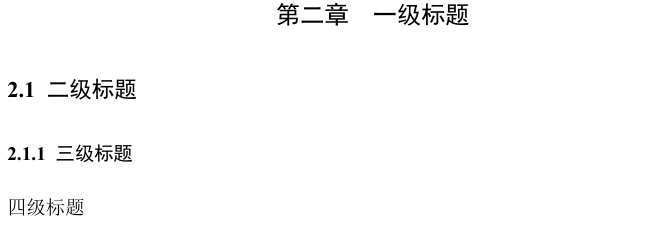
\includegraphics[width=0.5 \linewidth]{figures/2-1}
  \caption{标题格式}
  \label{2:1}
\end{figure}
\section{常用命令}
\subsection{分页}
分页包裹连续分页和奇数页分页,分别对应命令 \verb|\clearpage| 和 \verb|\cleardoublepage|,其中,\verb|\clearpage| 在空白页不会显示页眉页脚
\subsection{文本装饰}
\begin{lstlisting}[caption=文本装饰]
  \CJKunderdot{汉字,下加点} \\
  \CJKunderline{汉字,下划线} \\
  \CJKunderdblline{汉字,双下划线} \\
  \CJKunderwave{汉字,下波浪线} \\
  \CJKsout{汉字,删除线} \\
  \CJKxout{汉字,删除线}
\end{lstlisting}
\begin{center}
  \fbox{
    \parbox{8em}{
      \CJKunderdot{汉字,下加点} \\
      \CJKunderline{汉字,下划线} \\
      \CJKunderdblline{汉字,双下划线} \\
      \CJKunderwave{汉字,下波浪线} \\
      \CJKsout{汉字,删除线} \\
      \CJKxout{汉字,删除线}
    }
  }
\end{center}

\subsection{列表环境}
\LaTeX 提供了三种列表环境:编号的 enumerate 环境,不编号的 itemize 环境和使用关键字的 description 环境。在列表环境内部使用 \verb|\item| 命令开始一个列表项,他可以带一个可选参数表示手动编号或关键字。

enumerate 环境使用数字自动编号:
\clearpage
\begin{lstlisting}[caption=enumerate环境]
  \begin{enumerate}
    \item 中文
    \item English
    \item 日本語
  \end{enumerate}
\end{lstlisting}

\begin{center}
  \fbox{
    \parbox{8em}{
      \begin{enumerate}
        \item 中文
        \item English
        \item 日本語
      \end{enumerate}
    }
  }
\end{center}
itemize 环境不编号,但会在每个条目前加一个符号以示标记:
\begin{lstlisting}[caption=enumerate环境]
  \begin{itemize}
    \item 中文
    \item English
    \item 日本語
  \end{itemize}
\end{lstlisting}

\begin{center}
  \fbox{
    \parbox{8em}{
      \begin{itemize}
        \item 中文
        \item English
        \item 日本語
      \end{itemize}
    }
  }
\end{center}
description 环境总是使用 \verb|\item| 命令的可选参数,把它作为条目关键字加粗显示:
\clearpage
\begin{lstlisting}[caption=enumerate环境]
    \begin{description}
        \item[中文] 中国的语言文学 
        \item[English] The language of England
        \item[日本語] 日本の言語
    \end{description}
\end{lstlisting}

\begin{center}
  \fbox{
    \parbox{14em}{
      \begin{description}
        \item[中文] 中国的语言文学 
        \item[English] The language of England
        \item[日本語] 日本の言語
      \end{description}
    }
  }
\end{center}
这几个环境可以嵌套使用(至多四层),\LaTeX 会自动处理不同层次的缩进和编号。
  \chapter{参考文献}

\section{参考文件格式}
目前本模板仅有 ~{\color{blue}{GB/T~7714-2005}}~和~{\color{blue}{GB/T~7714-2015}}~样式,默认采用~{\color{blue}{GB/T~7714-2015}}~样式,如果需要使用其他格式,请自行寻找或编写 \emph{.bst}文件。

\section{BibTeX 的使用}
模板中有一个\emph{reference.bib}文件,是存放参考文献信息的数据库,通过谷歌学术、微软学术或是百度学术,查找文献时,把其 BibTeX 的引用信息复制到这个文件里,在你需要引用的地方,按照如下方式引用:
\begin{lstlisting}[caption=BibTeX 引用参考文献]
  \cite{bibid}  % bibid 就是你复制引文信息的第一个参数
  \cite{bibid1,bibid2,bibid2}  % 同时引用多个文献
\end{lstlisting}
  

\chapter{数学排版}
\section{行内和行间公式}
数学公式有两种排版方式:其一是与文字混排,称为\textbf{行内公式};其二是单独列为一行排版,称为行间公式。 

行内公式由一对 \texttt\$ 符号包裹:
\begin{lstlisting}
  $a^2 + b^2 = c^2$
\end{lstlisting}
\begin{center}
  \fbox{
    \parbox{10em}{
      \centering $a^2 + b^2 = c^2$
    }
  }
\end{center}
单独成行的行间公式在 \LaTeX{} 里由 equation 环境包裹。equation 环境为公式自动生成一个编号,这个编号可以用 \verb|\label| 和 \verb|\ref| 生成交叉引用,
amsmath 的 \verb|\eqref| 命令甚至为引用自动加上圆括号;还可以用 \verb|\tag| 命令手动修改公式的编号,或者用 \verb|\notag| 命令取消为公式编号。
\begin{lstlisting}[caption=多行公式示例一]
    The Pythagorean theorem is:
    \begin{equation}
      a^2 + b^2 = c^2 \label{pythagorean}
    \end{equation}
    Equation \eqref{pythagorean} is called `Gougu theorem' in Chinese.
\end{lstlisting}
\begin{center}
  \fbox{
    \parbox{30em}{
      The Pythagorean theorem is:
      \begin{equation}
      a^2 + b^2 = c^2 \label{pythagorean}
      \end{equation}
      Equation \eqref{pythagorean} is
      called `Gougu theorem' in Chinese.
    }
  }
\end{center}
\clearpage
\begin{lstlisting}[caption=多行公式示例二]
  It's wrong to say
  \begin{equation}
    1 + 1 = 3 \tag{dumb}
  \end{equation}
  or
  \begin{equation}
    1 + 1 = 4 \notag
  \end{equation}
\end{lstlisting}
\begin{center}
	\fbox{
		\parbox{30em}{
		    It's wrong to say
			\begin{equation}
			1 + 1 = 3 \tag{dumb}
			\end{equation}
			or
			\begin{equation}
			1 + 1 = 4 \notag
			\end{equation}
		}
	}
\end{center}

如果需要直接使用不带编号的行间公式,则将公式用命令 \verb|\[| 和 \verb|\]| 包裹,与之等效的是 \verb|displaymath| 环境。有的人更喜欢 \verb|equation|$*$ 环境,体现了带星号和不带星号的环境之间的区别。

\begin{lstlisting}[caption=多行公式示例三]
  \begin{equation*}
    a^2 + b^2 = c^2
  \end{equation*}
  For short:
  \[ a^2 + b^2 = c^2 \]
  Or if you like the long one:
  \begin{displaymath}
    a^2 + b^2 = c^2
  \end{displaymath}
\end{lstlisting}
\clearpage
\begin{center}
	\fbox{
		\parbox{30em}{
			\begin{equation*}
			a^2 + b^2 = c^2
			\end{equation*}
			For short:
			\[ a^2 + b^2 = c^2 \]
			Or if you like the long one:
			\begin{displaymath}
			a^2 + b^2 = c^2
			\end{displaymath}
		}
	}
\end{center}

我们通过一个例子展示行内公式和行间公式的对比。为了与文字相适应,行内公式在排版大的公式元素(分式、巨算符等)时显得很“局促”:
\begin{lstlisting}[caption=综合示例]
  In text:
  $\lim_{n \to \infty} \sum_{k=1}^n \frac{1}{k^2} = \frac{\pi^2}{6}$.
  In display:
  \[
    \lim_{n \to \infty}
    \sum_{k=1}^n \frac{1}{k^2}
    = \frac{\pi^2}{6}
  \]
\end{lstlisting}
\begin{center}
	\fbox{
		\parbox{30em}{
			In text:
			$\lim_{n \to \infty} \sum_{k=1}^n \frac{1}{k^2} = \frac{\pi^2}{6}$.
			
			In display:
			\[
			  \lim_{n \to \infty}
			  \sum_{k=1}^n \frac{1}{k^2}
			  = \frac{\pi^2}{6}
			\]
		}
	}
\end{center}
\clearpage
\section{数学模式}
当用户使用 \$ 开启行内公式输入,或是使用 \verb|\[| 命令、equation 环境时,\LaTeX{} 就进入了数学模式。数学模式相比于文本模式有以下特点:
\begin{enumerate}
	\item 数学模式中输入的空格被忽略。数学符号的间距默认由符号的性质(关系符号、运算符等)决定。
	需要人为引入间距时,使用 \verb|\quad| 和 \verb|\qquad| 等命令。
	\item 不允许有空行(分段)。行间公式中也无法用 \verb|\\| 命令手动换行。排版多行公式需要用到其他公式环境。
	\item 所有的字母被当作数学公式中的变量处理,字母间距与文本模式不一致,也无法生成单词之间的空格。
\end{enumerate}
\section{数学符号}
\subsection{一般符号}
\begin{table}[htp]
	\centering
	\caption{希腊字母} 
	\begin{quote}\footnotesize%
		\verb|\Alpha|,\verb|\Beta| 等希腊字母符号不存在,因为它们和拉丁字母 A,B 等一模一样;
		小写字母里也不存在 \verb|\omicron|,直接用拉丁字母 $o$ 代替。
	\end{quote}
	\begin{symbols}{*4{cl}}
		\hline
		\SYM{\alpha}     & \SYM{\theta}     & \SYM{o}          & \SYM{\upsilon}  \\
		\SYM{\beta}      & \SYM{\vartheta}  & \SYM{\pi}        & \SYM{\phi}      \\
		\SYM{\gamma}     & \SYM{\iota}      & \SYM{\varpi}     & \SYM{\varphi}   \\
		\SYM{\delta}     & \SYM{\kappa}     & \SYM{\rho}       & \SYM{\chi}      \\
		\SYM{\epsilon}   & \SYM{\lambda}    & \SYM{\varrho}    & \SYM{\psi}      \\
		\SYM{\varepsilon}& \SYM{\mu}        & \SYM{\sigma}     & \SYM{\omega}    \\
		\SYM{\zeta}      & \SYM{\nu}        & \SYM{\varsigma}  &                 \\
		\SYM{\eta}       & \SYM{\xi}        & \SYM{\tau}       &                 \\[1ex]
		\SYM{\Gamma}     & \SYM{\Lambda}    & \SYM{\Sigma}     & \SYM{\Psi}      \\
		\SYM{\Delta}     & \SYM{\Xi}        & \SYM{\Upsilon}   & \SYM{\Omega}    \\
		\SYM{\Theta}     & \SYM{\Pi}        & \SYM{\Phi}       &                 \\[1ex]
		\AMSM{\varGamma} & \AMSM{\varLambda}& \AMSM{\varSigma}  & \AMSM{\varPsi}      \\
		\AMSM{\varDelta} & \AMSM{\varXi}    & \AMSM{\varUpsilon}& \AMSM{\varOmega}    \\
		\AMSM{\varTheta} & \AMSM{\varPi}    & \AMSM{\varPhi}    &                 \\
		\hline
	\end{symbols}
\end{table}
\clearpage
~\\
\begin{table}[H]
	\centering
	\caption{其他符号}
	\begin{symbols}{*4{cl}}
		\hline
		\SYM{\dots}       & \SYM{\cdots}      & \SYM{\vdots}      & \SYM{\ddots}     \\
		\SYM{\hbar}       & \SYM{\imath}      & \SYM{\jmath}      & \SYM{\ell}       \\
		\SYM{\Re}         & \SYM{\Im}         & \SYM{\aleph}      & \SYM{\wp}        \\
		\SYM{\forall}     & \SYM{\exists}     & \LSYM{\mho}       & \SYM{\partial}   \\
		\SYM{'}           & \SYM{\prime}      & \SYM{\emptyset}   & \SYM{\infty}     \\
		\SYM{\nabla}      & \SYM{\triangle}   & \LSYM{\Box}       & \LSYM{\Diamond}  \\
		\SYM{\bot}        & \SYM{\top}        & \SYM{\angle}      & \SYM{\surd}      \\
		\SYM{\diamondsuit} & \SYM{\heartsuit} & \SYM{\clubsuit}   & \SYM{\spadesuit} \\
		\SYM{\neg} or \verb|\lnot| & \SYM{\flat} & \SYM{\natural}    & \SYM{\sharp}     \\
		\hline
	\end{symbols}
\end{table}

\subsection{指数、上下标和导数}
在\LaTeX{}中一般用 $\^$ 和 $\_$ 标明上下标,如果上下标不是一个字符需要使用花括号包裹,否则只对上下标符号后第一个字符起作用。

导数符号 \texttt' (${}'$) 是一类特殊的上标,可以适当连用表示多阶导数,也可以在其后连用上标:
\begin{lstlisting}
  $f(x) = x^2 \quad f'(x) = 2x \quad f''^{2}(x) = 4$
\end{lstlisting}
\begin{center}
	\fbox{
		\parbox{20em}{
			\centering $f(x) = x^2 \quad f'(x) = 2x \quad f''^{2}(x) = 4$
		}
	}
\end{center}
\subsection{分式和根式}
分式使用 \verb|\frac|\{分子\}\{分母\} 来书写。分式的大小在行间公式中是正常大小,而在行内被极度压缩。
\begin{center}
	\fbox{
		\parbox{20em}{
			In display style:
			\[
			3/8 \qquad \frac{3}{8}
			\qquad \tfrac{3}{8}
			\]
			In text style:
			$1\frac{1}{2}$~hours \qquad
			$1\dfrac{1}{2}$~hours
		}
	}
\end{center}
一般的根式使用 \verb|\sqrt{...}|;表示 $n$ 次方根时写成 \verb|\sqrt[n]{...}|.
\begin{center}
	\fbox{
		\parbox{20em}{
			\centering
			$\sqrt{x} \Leftrightarrow x^{1/2}
			\quad \sqrt[3]{2}
			\quad \sqrt{x^{2} + \sqrt{y}}$
		}
	}
\end{center}
特殊的分式形式,如二项式结构,由 amsmath 宏包的 \verb|\binom| 命令生成:
\begin{lstlisting}
  Pascal's rule is
  \[
    \binom{n}{k} =\binom{n-1}{k} + \binom{n-1}{k-1}
  \]
\end{lstlisting}
\begin{center}
	\fbox{
		\parbox{20em}{
			Pascal's rule is
			\[
			\binom{n}{k} =\binom{n-1}{k} + \binom{n-1}{k-1}
			\]
		}
	}
\end{center}
\subsection{关系符}
\LaTeX{}常见的关系符号如下表所示,同时还提供了自定义二元关系符的命令 \verb|\stackrel|,用于将一个符号代价在原有的二元关系符之上:
\begin{lstlisting}
  \[
    f_n(x) \stackrel{*}{\approx} 1
  \]
\end{lstlisting}
\begin{center}
	\fbox{
		\parbox{20em}{
			\centering
			\[
			  f_n(x) \stackrel{*}{\approx} 1
			\]
		}
	}
\end{center}
\clearpage
~\\
\begin{table}[H]
	\centering
	\caption{二元关系符}
	\begin{quote}\footnotesize%
		所有的二元关系符都可以加 \verb|\not| 前缀得到相反意义的关系符,例如 \verb|\not=| 就得到不等号(同 \verb|\ne|)。
	\end{quote}
	\begin{symbols}{*3{cl}}
		\hline
		\SYM{<}              & \SYM{>}                    & \SYM{=}          \\
		\SYM{\leq} or \verb|\le|   & \SYM{\geq} or \verb|\ge| & \SYM{\equiv}     \\
		\SYM{\ll}            & \SYM{\gg}                  & \SYM{\doteq}     \\
		\SYM{\prec}          & \SYM{\succ}                & \SYM{\sim}       \\
		\SYM{\preceq}        & \SYM{\succeq}              & \SYM{\simeq}     \\
		\SYM{\subset}        & \SYM{\supset}              & \SYM{\approx}    \\
		\SYM{\subseteq}      & \SYM{\supseteq}            & \SYM{\cong}      \\
		\LSYM{\sqsubset}     & \LSYM{\sqsupset}           & \LSYM{\Join}     \\
		\SYM{\sqsubseteq}    & \SYM{\sqsupseteq}          & \SYM{\bowtie}    \\
		\SYM{\in}            & \SYM{\ni}, \verb|\owns|      & \SYM{\propto}    \\
		\SYM{\vdash}         & \SYM{\dashv}               & \SYM{\models}    \\
		\SYM{\mid}           & \SYM{\parallel}            & \SYM{\perp}      \\
		\SYM{\smile}         & \SYM{\frown}               & \SYM{\asymp}     \\
		\SYM{:}              & \SYM{\notin}               & \SYM{\neq} or \verb|\ne| \\
		\hline
	\end{symbols}
\end{table}

\begin{table}[H]
	\centering
	\caption{\AmS{} 二元关系符} 
	\begin{symbols}{*3{cl}}
		\hline
		\AMSSYM{\lessdot}           & \AMSSYM{\gtrdot}            & \AMSSYM{\doteqdot} \\
		\AMSSYM{\leqslant}          & \AMSSYM{\geqslant}          & \AMSSYM{\risingdotseq}     \\
		\AMSSYM{\eqslantless}       & \AMSSYM{\eqslantgtr}        & \AMSSYM{\fallingdotseq}    \\
		\AMSSYM{\leqq}              & \AMSSYM{\geqq}              & \AMSSYM{\eqcirc}           \\
		\AMSSYM{\lll} or \verb|\llless| & \AMSSYM{\ggg}               & \AMSSYM{\circeq}  \\
		\AMSSYM{\lesssim}           & \AMSSYM{\gtrsim}            & \AMSSYM{\triangleq}        \\
		\AMSSYM{\lessapprox}        & \AMSSYM{\gtrapprox}         & \AMSSYM{\bumpeq}           \\
		\AMSSYM{\lessgtr}           & \AMSSYM{\gtrless}           & \AMSSYM{\Bumpeq}           \\
		\AMSSYM{\lesseqgtr}         & \AMSSYM{\gtreqless}         & \AMSSYM{\thicksim}         \\
		\AMSSYM{\lesseqqgtr}        & \AMSSYM{\gtreqqless}        & \AMSSYM{\thickapprox}      \\
		\AMSSYM{\preccurlyeq}       & \AMSSYM{\succcurlyeq}       & \AMSSYM{\approxeq}         \\
		\AMSSYM{\curlyeqprec}       & \AMSSYM{\curlyeqsucc}       & \AMSSYM{\backsim}          \\
		\AMSSYM{\precsim}           & \AMSSYM{\succsim}           & \AMSSYM{\backsimeq}        \\
		\AMSSYM{\precapprox}        & \AMSSYM{\succapprox}        & \AMSSYM{\vDash}            \\
		\AMSSYM{\subseteqq}         & \AMSSYM{\supseteqq}         & \AMSSYM{\Vdash}            \\
		\AMSSYM{\shortparallel}     & \AMSSYM{\Supset}            & \AMSSYM{\Vvdash}           \\
		\AMSSYM{\blacktriangleleft} & \AMSSYM{\sqsupset}          & \AMSSYM{\backepsilon}      \\
		\AMSSYM{\vartriangleright}  & \AMSSYM{\because}           & \AMSSYM{\varpropto}        \\
		\AMSSYM{\blacktriangleright}& \AMSSYM{\Subset}            & \AMSSYM{\between}          \\
		\AMSSYM{\trianglerighteq}   & \AMSSYM{\smallfrown}        & \AMSSYM{\pitchfork}        \\
		\AMSSYM{\vartriangleleft}   & \AMSSYM{\shortmid}          & \AMSSYM{\smallsmile}       \\
		\AMSSYM{\trianglelefteq}    & \AMSSYM{\therefore}         & \AMSSYM{\sqsubset}         \\
		\hline
	\end{symbols}
\end{table}
\subsection{算符}
\begin{table}[htp]
	\centering
	\caption{二元运算符}
	\begin{symbols}{*3{cl}}
		\hline
		\SYM{+}              & \SYM{-}              &                     \\
		\SYM{\pm}            & \SYM{\mp}            & \SYM{\triangleleft} \\
		\SYM{\cdot}          & \SYM{\div}           & \SYM{\triangleright}\\
		\SYM{\times}         & \SYM{\setminus}      & \SYM{\star}         \\
		\SYM{\cup}           & \SYM{\cap}           & \SYM{\ast}          \\
		\SYM{\sqcup}         & \SYM{\sqcap}         & \SYM{\circ}         \\
		\SYM{\vee}, \verb|\lor| & \SYM{\wedge},\verb|\land|  & \SYM{\bullet}   \\
		\SYM{\oplus}         & \SYM{\ominus}        & \SYM{\diamond}      \\
		\SYM{\odot}          & \SYM{\oslash}        & \SYM{\uplus}        \\
		\SYM{\otimes}        & \SYM{\bigcirc}       & \SYM{\amalg}        \\
		\SYM{\bigtriangleup} &\SYM{\bigtriangledown}& \SYM{\dagger}       \\
		\LSYM{\lhd}          & \LSYM{\rhd}          & \SYM{\ddagger}      \\
		\LSYM{\unlhd}        & \LSYM{\unrhd}        & \SYM{\wr}           \\
		\hline
	\end{symbols}
\end{table}
\begin{table}[htp]
	\centering
	\caption{\hologo{AmS} 二元运算符} 
	\begin{symbols}{*3{cl}}
		\hline
		\AMSSYM{\dotplus}        & \AMSSYM{\centerdot}      &       \\
		\AMSSYM{\ltimes}         & \AMSSYM{\rtimes}         & \AMSSYM{\divideontimes} \\
		\AMSSYM{\doublecup}      & \AMSSYM{\doublecap}      & \AMSSYM{\smallsetminus} \\
		\AMSSYM{\veebar}         & \AMSSYM{\barwedge}       & \AMSSYM{\doublebarwedge}\\
		\AMSSYM{\boxplus}        & \AMSSYM{\boxminus}       & \AMSSYM{\circleddash}   \\
		\AMSSYM{\boxtimes}       & \AMSSYM{\boxdot}         & \AMSSYM{\circledcirc}   \\
		\AMSSYM{\intercal}       & \AMSSYM{\circledast}     & \AMSSYM{\rightthreetimes} \\
		\AMSSYM{\curlyvee}       & \AMSSYM{\curlywedge}     & \AMSSYM{\leftthreetimes} \\
		\hline
	\end{symbols}
\end{table}
$\nabla$(\verb|\nabla|) 和 $\partial$(\verb|\partial|) 也是常用的算符,虽然它们不属于二元算符。
\LaTeX{} 将数学函数的名称作为一个算符排版,字体为直立字体。
\vspace{2em}
\begin{table}[htp]
	\centering
	\caption{\LaTeX{} 作为算符的函数名称一览}
	\begin{tabular}{*{5}{p{5em}}}
		\hline
		\multicolumn{5}{c}{\textbf{不带上下限的算符}} \\
		\hline
		\verb|\sin| & \verb|\arcsin| & \verb|\sinh| & \verb|\exp| & \verb|\dim| \\
		\verb|\cos| & \verb|\arccos| & \verb|\cosh| & \verb|\log| & \verb|\ker| \\
		\verb|\tan| & \verb|\arctan| & \verb|\tanh| & \verb|\lg|  & \verb|\hom| \\
		\verb|\cot| & \verb|\arg|    & \verb|\coth| & \verb|\ln|  & \verb|\deg| \\
		\verb|\sec| & \verb|\csc|    & \\
		\hline
		\multicolumn{5}{c}{\textbf{带上下限的算符}} \\
		\hline
		\verb|\lim| & \verb|\limsup| & \verb|\liminf| & \verb|\sup| & \verb|\inf| \\
		\verb|\min| & \verb|\max|    & \verb|\det|    & \verb|\Pr|  & \verb|\gcd| \\
		\hline
	\end{tabular}
\end{table}
\clearpage
\begin{lstlisting}
  \[
    \lim_{x \rightarrow 0}
    \frac{\sin x}{x}=1
  \]
\end{lstlisting}
\begin{center}
	\fbox{
		\parbox{20em}{
			\centering
		    \[
			  \lim_{x \rightarrow 0}
			  \frac{\sin x}{x}=1
			\]
		}
	}
\end{center}
对于求模表达式,\LaTeX{} 提供了 \verb|\bmod| 和 \verb|\pmod| 命令,前者相当于一个二元运算符,后者作为同余表达式的后缀:
\begin{lstlisting}
  $a\bmod b \\
  x\equiv a \pmod{b}$
\end{lstlisting}
\begin{center}
	\fbox{
		\parbox{20em}{
		  $a\bmod b \\
		  x\equiv a \pmod{b}$
		}
	}
\end{center}
amsmath 还允许用户在导言区用 \verb|\DeclareMathOperator|定义自己的算符,其中带星号的命令定义带上下限的算符:
\begin{verbatim}
\DeclareMathOperator{\argh}{argh}
\DeclareMathOperator*{\nut}{Nut}
\end{verbatim}
\begin{lstlisting}
  \[\argh 3 = \nut_{x=1} 4x\]
\end{lstlisting}
\begin{center}
	\fbox{
		\parbox{20em}{
			\[\argh 3 = \nut_{x=1} 4x\]
		}
	}
\end{center}
\subsection{巨算符}
积分号 $\int$(\verb|\int|)、求和号 $\sum$ (\verb|\sum|) 等符号称为\textbf{巨算符}。巨算符在行内公式和行间公式的大小和形状有区别。
\begin{lstlisting}
  In text:
  $\sum_{i=1}^n \quad
  \int_0^{\frac{\pi}{2}} \quad
  \oint_0^{\frac{\pi}{2}} \quad
  \prod_\epsilon $ \\
  In display:
  \[\sum_{i=1}^n \quad
  \int_0^{\frac{\pi}{2}} \quad
  \oint_0^{\frac{\pi}{2}} \quad
  \prod_\epsilon \]
\end{lstlisting}
\begin{center}
	\fbox{
		\parbox{20em}{
			In text:
			$\sum_{i=1}^n \quad
			\int_0^{\frac{\pi}{2}} \quad
			\oint_0^{\frac{\pi}{2}} \quad
			\prod_\epsilon $ \\
			In display:
			\[\sum_{i=1}^n \quad
			\int_0^{\frac{\pi}{2}} \quad
			\oint_0^{\frac{\pi}{2}} \quad
			\prod_\epsilon \]
		}
	}
\end{center}
巨算符的上下标位置可由 \verb|\limits| 和 \verb|\nolimits| 调整,前者令巨算符类似 $\lim$ 或求和算符 $\sum$,上下标位于上下方;后者令巨算符类似积分号,上下标位于右上方和右下方。

\begin{lstlisting}
  In text:
  $\sum\limits_{i=1}^n \quad
  \int\limits_0^{\frac{\pi}{2}} \quad
  \prod\limits_\epsilon $ \\
  In display:
  \[\sum\nolimits_{i=1}^n \quad
  \int\limits_0^{\frac{\pi}{2}} \quad
  \prod\nolimits_\epsilon \]
\end{lstlisting}
\begin{center}
	\fbox{
		\parbox{20em}{
			In text:
			$\sum\limits_{i=1}^n \quad
			\int\limits_0^{\frac{\pi}{2}} \quad
			\prod\limits_\epsilon $ \\
			In display:
			\[\sum\nolimits_{i=1}^n \quad
			\int\limits_0^{\frac{\pi}{2}} \quad
			\prod\nolimits_\epsilon \]
		}
	}
\end{center}
amsmath 宏包还提供了 \verb|\substack|,能够在下限位置书写多行表达式;subarray
环境更进一步,令多行表达式可选择居中 (c) 或左对齐 (l):
\begin{lstlisting}
  \[
  \sum_{\substack{0\le i\le n \\
  j\in \mathbb{R}}}
  P(i,j) = Q(n)
  \]
  \[
  \sum_{\begin{subarray}{l}
  0\le i\le n \\
  j\in \mathbb{R}
  \end{subarray}}
  P(i,j) = Q(n)
  \]
\end{lstlisting}
\begin{center}
	\fbox{
		\parbox{20em}{
			\[
			\sum_{\substack{0\le i\le n \\
					j\in \mathbb{R}}}
			P(i,j) = Q(n)
			\]
			\[
			\sum_{\begin{subarray}{l}
				0\le i\le n \\
				j\in \mathbb{R}
				\end{subarray}}
			P(i,j) = Q(n)
			\]
		}
	}
\end{center}
\clearpage
~\\
\begin{table}[H]
	\centering
	\caption{巨算符}
	\def\arraystretch{2.2}
	\begin{symbols}{*3{ccl}}
		\hline
		\BIGSYM{\sum}      & \BIGSYM{\bigcup}   & \BIGSYM{\bigvee}  \\
		\BIGSYM{\prod}     & \BIGSYM{\bigcap}   & \BIGSYM{\bigwedge} \\
		\BIGSYM{\coprod}   & \BIGSYM{\bigsqcup} & \BIGSYM{\biguplus} \\
		\BIGSYM{\int}      & \BIGSYM{\oint}     & \BIGSYM{\bigodot} \\
		\BIGSYM{\bigoplus} & \BIGSYM{\bigotimes} & \\
		\AMSBIG{\iint}     & \AMSBIG{\iiint}    & \AMSBIG{\iiiint}  \\
		\AMSBIG{\idotsint} &                    & \\
		\hline
	\end{symbols}
\end{table}
\subsection{数学重音和上下括号}
\begin{table}[htp]
	\centering
	\caption{数学重音符号}
	\begin{quote}\footnotesize%
		最后一个 \verb|\wideparen| 依赖 yhmath 宏包。
	\end{quote}
	\begin{symbols}{*3{cl}}
		\hline
		\ACC{\hat}{a}   & \ACC{\check}{a} & \ACC{\tilde}{a}       \\
		\ACC{\acute}{a} & \ACC{\grave}{a} & \ACC{\breve}{a}       \\
		\ACC{\bar}{a}   & \ACC{\vec}{a}   & \ACC{\mathring}{a}    \\
		\ACC{\dot}{a}   & \ACC{\ddot}{a}  & \AMSACC{\dddot}{a}    \\
		\AMSACC{\ddddot}{a} \\[1ex]
		\ACC{\widehat}{AAA} & \ACC{\widetilde}{AAA} & \ACC{\wideparen}{AAA} \\
		\hline
	\end{symbols}
\end{table}

\begin{table}[htp]
	\centering
	\caption{作为重音的箭头符号} 
	\begin{symbols}{*2{cl}}
		\hline
		\ACC{\overrightarrow}{AB}     & \AMSACC{\underrightarrow}{AB}     \\
		\ACC{\overleftarrow}{AB}      & \AMSACC{\underleftarrow}{AB}      \\
		\AMSACC{\overleftrightarrow}{AB} & \AMSACC{\underleftrightarrow}{AB} \\
		\hline
	\end{symbols}
\end{table}

\cmd{overbrace} 和 \cmd{underbrace} 命令用来生成上/下括号,各自可带一个上/下标公式。
\begin{lstlisting}
  $\underbrace{\overbrace{(a+b+c)}^6
  \cdot \overbrace{(d+e+f)}^7}
  _\text{meaning of life} = 42$
\end{lstlisting}

\begin{center}
	\fbox{
		\parbox{20em}{
			\centering
			$\underbrace{\overbrace{(a+b+c)}^6
				\cdot \overbrace{(d+e+f)}^7}
			_\text{meaning of life} = 42$
		}
	}
\end{center}

\subsection{箭头}
常用的箭头包括 \cmd{rightarrow} ($\rightarrow$,或 \cmd{to})、\cmd{leftarrow}($\leftarrow$,或 \cmd{gets})等。
\begin{table}[H]
	\centering
	\caption{箭头}
	\begin{symbols}{*2{cl}}
		\hline
		\SYM{\leftarrow} or \cmd{gets} & \SYM{\longleftarrow} \\
		\SYM{\rightarrow} or \cmd{to}   & \SYM{\longrightarrow} \\
		\SYM{\leftrightarrow}    & \SYM{\longleftrightarrow} \\
		\SYM{\Leftarrow}         & \SYM{\Longleftarrow}     \\
		\SYM{\Rightarrow}        & \SYM{\Longrightarrow}    \\
		\SYM{\Leftrightarrow}    & \SYM{\Longleftrightarrow}\\
		\SYM{\mapsto}            & \SYM{\longmapsto}        \\
		\SYM{\hookleftarrow}     & \SYM{\hookrightarrow}    \\
		\SYM{\leftharpoonup}     & \SYM{\rightharpoonup}    \\
		\SYM{\leftharpoondown}   & \SYM{\rightharpoondown}  \\
		\SYM{\rightleftharpoons} & \SYM{\iff}               \\
		\SYM{\uparrow}           & \SYM{\downarrow} \\
		\SYM{\updownarrow}       & \SYM{\Uparrow} \\
		\SYM{\Downarrow}         & \SYM{\Updownarrow} \\
		\SYM{\nearrow}           & \SYM{\searrow} \\
		\SYM{\swarrow}           & \SYM{\nwarrow} \\
		\LSYM{\leadsto}          &              \\
		\hline
	\end{symbols}
\end{table}
amsmath 的 \cmd{xleft\-arrow} 和 \cmd{xright\-arrow} 命令提供了长度可以伸展的箭头,并且可以为箭头增加上下标:
\begin{lstlisting}
  \[ a\xleftarrow{x+y+z} b \]
  \[ c\xrightarrow[x<y]{a*b*c}d \]
\end{lstlisting}
\begin{center}
	\fbox{
		\parbox{20em}{
			 \[ a\xleftarrow{x+y+z} b \]
			\[ c\xrightarrow[x<y]{a*b*c}d \]
		}
	}
\end{center}

\subsection{括号和定界符}

\begin{table}[htp]
	\centering
	\caption{定界符}
	\begin{quote}\footnotesize%
		amsmath 还定义了 \cmd{lvert}、\cmd{rvert} 和 \cmd{lVert}、\cmd{rVert},
		分别作为 \cmd{vert} 和 \cmd{Vert} 对应的开符号(左侧)和闭符号(右侧)的命令。
	\end{quote}
	\begin{symbols}{*4{cl}}
		\hline
		\SYM{(}                  & \SYM{)}                  & \SYM{\uparrow}     & \SYM{\downarrow}   \\
		\SYM{[}  or \cmd{lbrack} & \SYM{]}  or \cmd{rbrack} & \SYM{\Uparrow}     & \SYM{\Downarrow}   \\
		\SYM{\{} or \cmd{lbrace} & \SYM{\}} or \cmd{rbrace} & \SYM{\updownarrow} & \SYM{\Updownarrow} \\
		\SYM{|}  or \cmd{vert}   & \SYM{\|} or \cmd{Vert}   & \SYM{\lceil}       & \SYM{\rceil}       \\
		\SYM{\langle}            & \SYM{\rangle}            & \SYM{\lfloor}      & \SYM{\rfloor}      \\
		\SYM{/}                  & \SYM{\backslash} \\
		\hline
	\end{symbols}
\end{table}

\begin{table}[htp]
	\centering
	\caption{用于行间公式的大定界符}
	\def\arraystretch{1.8}
	\begin{symbols}{*3{cl}}
		\hline
		\DEL{\lgroup}      & \DEL{\rgroup}      & \DEL{\lmoustache}  \\
		\DEL{\arrowvert}   & \DEL{\Arrowvert}   & \DEL{\bracevert} \\
		\DEL{\rmoustache} \\
		\hline
	\end{symbols}
\end{table}

使用 \cmd{left} 和 \cmd{right} 命令可令括号(定界符)的大小可变,在行间公式中常用。\LaTeX{} 会自动根据括号内的公式大小决定定界符大小。
\cmd{left} 和 \cmd{right} 必须成对使用。需要使用单个定界符时,另一个定界符写成 \cmd{left.} 或 \cmd{right.}。

\begin{lstlisting}
  \[1 + \left(\frac{1}{1-x^{2}}
  \right)^3 \qquad
  \left.\frac{\partial f}{\partial t}
  \right|_{t=0}\]
\end{lstlisting}

\begin{center}
	\fbox{
		\parbox{20em}{
			\[1 + \left(\frac{1}{1-x^{2}}
			\right)^3 \qquad
			\left.\frac{\partial f}{\partial t}
			\right|_{t=0}\] 
		}
	}
\end{center}
有时我们不满意于 \LaTeX{} 为我们自动调节的定界符大小。这时我们还可以用 \cmd{big}、\cmd{bigg} 等命令生成固定大小的定界符。
更常用的形式是类似 \cmd{left} 的 \cmd{bigl}、\cmd{biggl} 等,以及类似 \cmd{right} 的 \cmd{bigr}、\cmd{biggr} 等
(\cmd{bigl} 和 \cmd{bigr} 不必成对出现)。
\begin{lstlisting}
  $\Bigl((x+1)(x-1)\Bigr)^{2}$\\
  $\bigl( \Bigl( \biggl( \Biggl( \quad
  \bigr\} \Bigr\} \biggr\} \Biggr\} \quad
  \big\| \Big\| \bigg\| \Bigg\| \quad
  \big\Downarrow \Big\Downarrow
  \bigg\Downarrow \Bigg\Downarrow$
\end{lstlisting}
\begin{center}
	\fbox{
		\parbox{20em}{
			$\Bigl((x+1)(x-1)\Bigr)^{2}$\\
			$\bigl( \Bigl( \biggl( \Biggl( \quad
			\bigr\} \Bigr\} \biggr\} \Biggr\} \quad
			\big\| \Big\| \bigg\| \Bigg\| \quad
			\big\Downarrow \Big\Downarrow
			\bigg\Downarrow \Bigg\Downarrow$
		}
	}
\end{center}

\section{多行公式}
\subsection{长公式折行}
通常来讲应当避免写出超过一行而需要折行的长公式。如果一定要折行的话,习惯上优先在等号之前折行,其次在加号、减号之前,再次在乘号、除号之前。
其它位置应当避免折行。

amsmath 宏包的 multline 环境提供了书写折行长公式的方便环境。
它允许用 \crcmd{} 折行,将公式编号放在最后一行。
多行公式的首行左对齐,末行右对齐,其余行居中。
\begin{lstlisting}
  \begin{multline}
    a + b + c + d + e + f
    + g + h + i \\
    = j + k + l + m + n\\
    = o + p + q + r + s\\
    = t + u + v + x + z
  \end{multline}
\end{lstlisting}
\begin{center}
	\fbox{
		\parbox{20em}{
			\begin{multline}
			a + b + c + d + e + f
			+ g + h + i \\
			= j + k + l + m + n\\
			= o + p + q + r + s\\
			= t + u + v + x + z 
			\end{multline}
		}
	}
\end{center}

\subsection{多行公式}
更多的情况是,我们需要罗列一系列公式,并令其按照等号对齐。目前最常用的是 align 环境,它将公式用 \texttt\& 隔为两部分并对齐。分隔符通常放在等号左边:
\begin{lstlisting}
  \begin{align}
    a & = b + c \\
      & = d + e
  \end{align}
\end{lstlisting}
\begin{center}
	\fbox{
		\parbox{20em}{
			\begin{align}
			a & = b + c \\
			& = d + e
			\end{align}
		}
	}
\end{center}
align 环境会给每行公式都编号。我们仍然可以用 \cmd{notag} 去掉某行的编号。
在以下的例子,为了对齐等号,我们将分隔符放在右侧,并且此时需要在等号后添加一对括号 \texttt\{\texttt\} 以产生正常的间距:
\begin{lstlisting}
  \begin{align}
  a ={} & b + c \\
  ={} & d + e + f + g + h + i
  + j + k + l \notag \\
  & + m + n + o \\
  ={} & p + q + r + s
  \end{align}
\end{lstlisting}
\begin{center}
	\fbox{
		\parbox{20em}{
			\begin{align}
			a ={} & b + c \\
			={} & d + e + f + g + h + i
			+ j + k + l \notag \\
			& + m + n + o \\
			={} & p + q + r + s
			\end{align}
		}
	}
\end{center}
align 还能够对齐多组公式,除等号前的 \texttt\& 之外,公式之间也用 \texttt\& 分隔:
\begin{lstlisting}
  \begin{align}
  a &=1  &  b &=2   & c &=3   \\
  d &=-1 &  e &=-2  & f &=-5
  \end{align}
\end{lstlisting}
\begin{center}
	\fbox{
		\parbox{20em}{
			\begin{align}
			a &=1  &  b &=2   & c &=3   \\
			d &=-1 &  e &=-2  & f &=-5
			\end{align}
		}
	}
\end{center}
如果我们不需要按等号对齐,只需罗列数个公式,gather 将是一个很好用的环境:
\begin{lstlisting}
\begin{gather}
a = b + c \\
d = e + f + g \\
h + i = j + k \notag \\
l + m = n
\end{gather}
\end{lstlisting}
\begin{center}
	\fbox{
		\parbox{20em}{
			\begin{gather}
			a = b + c \\
			d = e + f + g \\
			h + i = j + k \notag \\
			l + m = n
			\end{gather}
		}
	}
\end{center}
\subsection{公用编号的多行公式}
另一个常见的需求是将多个公式组在一起公用一个编号,编号位于公式的居中位置。为此,amsmath 宏包
提供了诸如 aligned、gathered 等环境,与 equation 环境套用。
以 \texttt{-ed} 结尾的环境用法与前一节不以 \texttt{-ed} 结尾的环境用法一一对应。我们仅以 aligned 举例:
\begin{lstlisting}
  \begin{equation}
	  \begin{aligned}
		  a &= b + c \\
		  d &= e + f + g \\
		  h + i &= j + k \\
		  l + m &= n
	  \end{aligned}
  \end{equation}
\end{lstlisting}
\begin{center}
	\fbox{
		\parbox{20em}{
			\begin{equation}
				\begin{aligned}
					a &= b + c \\
					d &= e + f + g \\
					h + i &= j + k \\
					l + m &= n
				\end{aligned}
			\end{equation}
		}
	}
\end{center}
\section{数组和矩阵}
为了排版二维数组,\LaTeX{} 提供了 \env{array} 环境,用法与 \env{tabular} 环境极为类似,也需要定义列格式,并用 \crcmd{} 换行。
数组可作为一个公式块,在外套用 \cmd{left}、\cmd{right} 等定界符:

\begin{lstlisting}
  \[ \mathbf{X} = \left(
    \begin{array}{cccc}
    x_{11} & x_{12} & \ldots & x_{1n}\\
    x_{21} & x_{22} & \ldots & x_{2n}\\
    \vdots & \vdots & \ddots & \vdots\\
    x_{n1} & x_{n2} & \ldots & x_{nn}\\
    \end{array} 
  \right) \]
\end{lstlisting}
\begin{center}
	\fbox{
		\parbox{25em}{
			\[ \mathbf{X} = \left(
			\begin{array}{cccc}
			x_{11} & x_{12} & \ldots & x_{1n}\\
			x_{21} & x_{22} & \ldots & x_{2n}\\
			\vdots & \vdots & \ddots & \vdots\\
			x_{n1} & x_{n2} & \ldots & x_{nn}\\
			\end{array} 
			\right) \]
		}
	}
\end{center}
我们还可以利用空的定界符排版出这样的效果:
\begin{lstlisting}
  \[ |x| = \left\{
    \begin{array}{rl}
      -x & \text{if } x < 0,\\
      0 & \text{if } x = 0,\\
      x & \text{if } x > 0.
    \end{array} \right. 
  \]
\end{lstlisting}
\begin{center}
	\fbox{
		\parbox{25em}{
			\[ |x| = \left\{
			\begin{array}{rl}
			-x & \text{if } x < 0,\\
			0 & \text{if } x = 0,\\
			x & \text{if } x > 0.
			\end{array} \right. 
			\]
		}
	}
\end{center}
不过上述例子可以用 amsmath 提供的 \env{cases} 环境更轻松地完成:
\begin{lstlisting}
  \[ |x| =
    \begin{cases}
      -x & \text{if } x < 0,\\
      0 & \text{if } x = 0,\\
      x & \text{if } x > 0.
    \end{cases} 
  \]
\end{lstlisting}
\begin{center}
	\fbox{
		\parbox{25em}{
			  \[ |x| =
			\begin{cases}
			-x & \text{if } x < 0,\\
			0 & \text{if } x = 0,\\
			x & \text{if } x > 0.
			\end{cases} 
			\]
		}
	}
\end{center}
我们当然也可以用 \env{array} 环境排版各种矩阵。amsmath 宏包还直接提供了多种排版矩阵的环境,包括不带定界符的 \env{matrix},
以及带各种定界符的矩阵 \env{pmatrix}($\bigl($)、\env{bmatrix}($\bigl[$)、\env{Bmatrix}($\bigl\{$)、
\env{vmatrix}($\bigl\vert$)、\env{Vmatrix}($\bigl\Vert$)。使用这些环境时,无需给定列格式:
\begin{lstlisting}
  \[
  \begin{matrix}
  1 & 2 \\ 3 & 4
  \end{matrix} \qquad
  \begin{bmatrix}
  x_{11} & x_{12} & \ldots & x_{1n}\\
  x_{21} & x_{22} & \ldots & x_{2n}\\
  \vdots & \vdots & \ddots & \vdots\\
  x_{n1} & x_{n2} & \ldots & x_{nn}\\
  \end{bmatrix}
  \]
\end{lstlisting}
\begin{center}
	\fbox{
		\parbox{25em}{
			  \[
			\begin{matrix}
			1 & 2 \\ 3 & 4
			\end{matrix} \qquad
			\begin{bmatrix}
			x_{11} & x_{12} & \ldots & x_{1n}\\
			x_{21} & x_{22} & \ldots & x_{2n}\\
			\vdots & \vdots & \ddots & \vdots\\
			x_{n1} & x_{n2} & \ldots & x_{nn}\\
			\end{bmatrix}
			\]
		}
	}
\end{center}
\section{公式中的间距}
绝大部分时候,数学公式中各元素的间距是根据符号类型自动生成的,需要我们手动调整的情况极少。
我们已经认识了两个生成间距的命令 \cmd{quad} 和 \cmd{qquad}。在公式中我们还可能用到的间距包括 \cmd{,}、\cmd{:}、\cmd{;}
以及负间距 \cmd{!},其中 \cmd{quad} 、 \cmd{qquad} 和 \cmd{,} 在文本和数学环境中可用,后三个命令只用于数学环境。
文本中的 \cmd{\textvisiblespace} 也能使用在数学公式中。

\newdimen\testdimen \testdimen=\fontdimen6\textfont2 \divide\testdimen18\relax
\begin{center}
	\begin{tabularx}{0.9\textwidth}{*{3}{>{\raggedright\arraybackslash}X}|*{3}{>{\raggedright\arraybackslash}X}}
		\hline
		无额外间距  &                          & $a a$        &
		\cmd{,}     & \demowidth{3\testdimen}  & $a\,a$       \\
		\cmd{quad}  & \demowidth{18\testdimen} & $a\quad a$   &
		\cmd{:}     & \demowidth{4\testdimen}  & $a\:a$       \\
		\cmd{qquad} & \demowidth{36\testdimen} & $a\qquad a$  &
		\cmd{;}     & \demowidth{5\testdimen}  & $a\;a$       \\
		\cmd{\textvisiblespace}     & \demowidth{\fontdimen2\textfont0} & $a\ a$ &
		\cmd{!}     & $-$\demowidth{3\testdimen} & $a\!a$     \\
		\hline
	\end{tabularx}
\end{center}
一个常见的用途是修正积分的被积函数$f(x)$和微元$\mathrm{d}x$之间的距离。注意微元里的$\mathrm{d}$用的是直立体:
\begin{lstlisting}
  \[
  \int_a^b f(x)\mathrm{d}x
  \qquad
  \int_a^b f(x)\,\mathrm{d}x
  \]
\end{lstlisting}
\begin{center}
	\fbox{
		\parbox{20em}{
			  \[
			\int_a^b f(x)\mathrm{d}x
			\qquad
			\int_a^b f(x)\,\mathrm{d}x
			\]
		}
	}
\end{center}

\section{数学符号的字体控制}
\subsection{数学字母字体}
\LaTeX{} 允许一部分数学符号切换字体,主要是拉丁字母、数字、大写希腊字母以及重音符号等。
表 \ref{tbl:math-fonts} 给出了切换字体的命令。某一些命令需要字体宏包的支持。
\begin{table}[htp]
	\centering
	\caption{数学字母字体} \label{tbl:math-fonts}
	\begin{tabular}{*{3}{l}}
		\hline
		\textbf{示例}    & \textbf{命令} & \textbf{依赖的宏包}\\
		\hline
		$\mathnormal{ABCDE abcde 1234}$  & \cmd{mathnormal}\marg*{\ldots}&       \\
		$\mathrm{ABCDE abcde 1234}$      & \cmd{mathrm}\marg*{\ldots}    &       \\
		$\mathit{ABCDE abcde 1234}$      & \cmd{mathit}\marg*{\ldots}    &       \\
		$\mathbf{ABCDE abcde 1234}$      & \cmd{mathbf}\marg*{\ldots}    &       \\
		$\mathsf{ABCDE abcde 1234}$      & \cmd{mathsf}\marg*{\ldots}    &       \\
		$\mathtt{ABCDE abcde 1234}$      & \cmd{mathtt}\marg*{\ldots}    &       \\
		$\CMcal{ABCDE}$                  & \cmd{mathcal}\marg*{\ldots}   & 仅提供大写字母 \\
		\hline
		$\EuScript{ABCDE}$               & \cmd{mathcal}\marg*{\ldots}   & eucal 仅提供大写字母 \\
		$\mathscr{ABCDE}$                & \cmd{mathscr}\marg*{\ldots}   & mathrsfs 仅提供大写字母\\
		$\mathfrak{ABCDE abcde 1234}$    & \cmd{mathfrak}\marg*{\ldots}  & amssymb 或 eufrak  \\
		$\mathbb{ABCDE}$                 & \cmd{mathbb}\marg*{\ldots}    & amssymb 仅提供大写字母 \\
		\hline
	\end{tabular}
\end{table}

\subsection{数学符号的尺寸}
数学符号按照符号排版的位置规定尺寸,从大到小包括行间公式尺寸、行内公式尺寸、上下标尺寸、次级上下标尺寸。
除了字号有别之外,行间和行内公式尺寸下的巨算符也使用不一样的大小。\LaTeX{} 为每个数学尺寸指定了一个切换的命令,见表 \ref{tbl:math-size}。

\begin{table}[htp]
	\centering
	\caption{数学符号尺寸}\label{tbl:math-size}
	\begin{tabular}{lll}
		\hline
		\textbf{命令} & \textbf{尺寸} & \textbf{示例} \\
		\hline
		\cmd{displaystyle}      & 行间公式尺寸   & $\displaystyle\sum a $\\
		\cmd{textstyle}         & 行内公式尺寸   & $\textstyle\sum a $ \\
		\cmd{scriptstyle}       & 上下标尺寸     & $\scriptstyle a$ \\
		\cmd{scriptscriptstyle} & 次级上下标尺寸 & $\scriptscriptstyle a$\\
		\hline
	\end{tabular}
\end{table}
我们通过以下示例对比行间公式和行内公式的区别。在分式中,分子分母默认为行内公式尺寸,示例中将分母切换到行间公式尺寸:
\clearpage
\begin{lstlisting}
  \[
    r = \frac
    {\sum_{i=1}^n (x_i- x)(y_i- y)}
    {\displaystyle \left[
    \sum_{i=1}^n (x_i-x)^2
    \sum_{i=1}^n (y_i-y)^2
    \right]^{1/2} }
  \]
\end{lstlisting}
\begin{center}
	\fbox{
		\parbox{20em}{
			\[
			r = \frac
			{\sum_{i=1}^n (x_i- x)(y_i- y)}
			{\displaystyle \left[
				\sum_{i=1}^n (x_i-x)^2
				\sum_{i=1}^n (y_i-y)^2
				\right]^{1/2} }
			\]
		}
	}
\end{center}



















  \chapter{插入图片}
\section{基本使用}
\LaTeX{} 本身不支持插图功能,需要由 \pkg{graphicx} 宏包辅助支持。
在调用了 \pkg{graphicx} 宏包以后,就可以使用 \cmd{include\-graphics} 命令加载图片了:
\begin{lstlisting}
	\includegraphics[<options>]{<filename>}
\end{lstlisting}
其中 \Arg{filename} 为图片文件名,与 \cmd{include} 命令的用法类似,文件名可能需要用相对路径或绝对路径表示。图片文件的扩展名一般可不写。另外一定要注意,\textbf{文件名里既不要有空格(类似 \cmd{include}),也不要有多余的英文点号},否则宏包在解析文件名的过程中会出错。

另外 \pkg{graphicx} 宏包还提供了 \cmd{graphics\-path} 命令,用于声明一个或多个图片文件存放的目录,
使用这些目录里的图片时可不用写路径:
\begin{lstlisting}
  % 假设主要的图片放在 figures 子目录下,标志放在 logo 子目录下
  \graphicspath{{figures/}{logo/}}
\end{lstlisting}

\cmd{includegraphics} 命令的可选参数 \Arg{options} 支持 \Arg{key}=\Arg{value} 形式赋值,常用的参数如下:
\begin{table}[htp]
	\centering
	\caption{\cmd{includegraphics} 命令的可选参数}\label{tbl:graphics-options}
	\begin{tabular}{lp{18em}}
		\hline
		\textbf{参数} & \textbf{含义} \\
		\hline
		\texttt{width=}\Arg{width}    &  将图片缩放到宽度为 \Arg{width} \\
		\texttt{height=}\Arg{height}  &  将图片缩放到高度为 \Arg{height} \\
		\texttt{scale=}\Arg{scale}    &  将图片相对于原尺寸缩放 \Arg{scale} 倍 \\
		\texttt{angle=}\Arg{angle}    &  令图片逆时针旋转 \Arg{angle} 度 \\
		\hline
	\end{tabular}
\end{table}
\clearpage
\section{排版多行多列图片}
这里给个离职,模仿写就好:
\begin{lstlisting}
  \begin{figure}[htbp]
    \centering
    \includegraphics[width=...]{...}
    \qquad
    \includegraphics[width=...]{...} \\[..pt]
    \includegraphics[width=...]{...}
    \caption{...}
    \label{...}
  \end{figure}
\end{lstlisting}
\begin{figure}[htp]
	\centering
	\fcolorbox[gray]{0}{0.96}{\parbox{10em}{\vrule width 0pt height 10ex\hfil}}
	\qquad
	\fcolorbox[gray]{0}{0.96}{\parbox{10em}{\vrule width 0pt height 12ex\hfil}}
	\par\bigskip
	\fcolorbox[gray]{0}{0.96}{\parbox{20em}{\vrule width 0pt height 12ex\hfil}}
	\caption{并排放置图片的示意。}\label{fig:parallel-fig}
\end{figure}
或者使用这种方式,个人比较喜欢下面这种:
\clearpage
\begin{lstlisting}
  \begin{figure}[t]
    \centering
    \subfloat[图1]{
      \label{fig1}
      \includegraphics[width=0.5\textwidth]{图1}
    }
    \subfloat[图2]{
      \label{fig2}
      \includegraphics[width=0.5\textwidth]{图2}
    }\\ 
    \subfloat[图3]{
      \label{fig3}
      \includegraphics[width=0.5\textwidth]{图3}
    } 
    \subfloat[图4]{
      \label{fig4}
      \includegraphics[width=0.5\textwidth]{图4}
    }
    \caption{多行多列子图}
    \label{fig}	
  \end{figure}
\end{lstlisting}
\begin{figure}[H]
	\centering
	\subfloat[图1]{
		\label{fig1}
		\fcolorbox[gray]{0}{0.96}{\parbox{10em}{\vrule width 0pt height 10ex\hfil}}
	}% 
	\subfloat[图2]{
		\label{fig2}
		\fcolorbox[gray]{0}{0.96}{\parbox{10em}{\vrule width 0pt height 10ex\hfil}}
	}\\ 
	\subfloat[图3]{
		\label{fig3}
		\fcolorbox[gray]{0}{0.96}{\parbox{10em}{\vrule width 0pt height 10ex\hfil}}
	} 
	\subfloat[图4]{
		\label{fig4}
		\fcolorbox[gray]{0}{0.96}{\parbox{10em}{\vrule width 0pt height 10ex\hfil}}
	}
	\caption{多行多列子图}
	\label{fig}	
\end{figure}
  \chapter{插入表格}
\LaTeX{} 里排版表格不如 Word 等所见即所得的工具简便和自由,不过对于不太复杂的表格来讲,完全能够胜任。

排版表格最基本的 \env{tabular} 环境用法为:
\begin{lstlisting}
  \begin{tabular}[align]{column-spec}
    <item1> & <item2> & ... \\
    \hline
    <item1> & <item2> & ... \\
  \end{tabular}
\end{lstlisting}
其中 \Arg{column-spec} 是列格式标记,在接下来的内容将仔细介绍;\texttt\& 用来分隔单元格;
\crcmd{} 用来换行;\cmd{hline} 用来在行与行之间绘制横线。


直接使用 \env{tabular} 环境的话,会\textbf{和周围的文字混排}。此时可用一个可选参数 \Arg{align} 控制垂直对齐:
\verb|t| 和 \verb|b| 分别表示按表格顶部、底部对齐,其他参数或省略不写(默认)表示居中对齐。
\begin{lstlisting}
  \begin{tabular}{|c|}
  center-\\ aligned \\
  \end{tabular},
  
  \begin{tabular}[t]{|c|}
  top-\\ aligned \\
  \end{tabular},
  
  \begin{tabular}[b]{|c|}
  bottom-\\ aligned\\
  \end{tabular} tabulars.
\end{lstlisting}
\begin{center}
	\fbox{
		\parbox{30em}{
			\centering
			\begin{tabular}{|c|}
				center-\\ aligned \\
			\end{tabular},
			\begin{tabular}[t]{|c|}
				top-\\ aligned \\
			\end{tabular},
			\begin{tabular}[b]{|c|}
				bottom-\\ aligned\\
			\end{tabular} tabulars.
		}
	}
\end{center}

但是通常情况下 \env{tabular} 环境很少与文字直接混排,而是会放在 \env{table} 浮动体环境中,并用 \cmd{caption} 命令加标题。

\section{列格式}
\env{tabular} 环境使用 \Arg{column-spec} 参数指定表格的列数以及每列的格式。
\begin{table}[htp]
	\centering
	\caption{\LaTeX{} 表格列格式}
	\begin{tabular}{*{2}{l}}
		\hline
		\textbf{列格式} & \textbf{说明} \\
		\hline
		\ttfamily l/c/r          & 单元格内容左对齐/居中/右对齐,不折行 \\
		\ttfamily p\marg{width}  & 单元格宽度固定为 \Arg{width},可自动折行 \\
		\ttfamily |              & 绘制竖线 \\
		\ttfamily @\marg{string} & 自定义内容 \Arg{string} \\
		\hline
	\end{tabular}
\end{table}

\begin{lstlisting}
  \begin{tabular}{lcr|p{6em}}
    \hline
    left & center & right
    & par box with fixed width\\
    L & C & R & P \\
    \hline
  \end{tabular}
\end{lstlisting}
\begin{center}
	\fbox{
		\parbox{20em}{
			\centering
			\begin{tabular}{lcr|p{6em}}
				\hline
				left & center & right
				& par box with fixed width\\
				L    & C      & R     & P \\
				\hline
			\end{tabular}
		}
	}
\end{center}

表格中每行的单元格数目不能多于列格式里 \texttt{l/c/r/p} 的总数(可以少于这个总数),否则出错。

\texttt{@} 格式可在单元格前后插入任意的文本,但同时它也消除了单元格前后额外添加的间距。
\texttt{@} 格式可以适当使用以充当“竖线”。特别地,\texttt{@}\marg*{} 可直接用来消除单元格前后的间距:
\clearpage
\begin{lstlisting}
  \begin{tabular}{@{} r@{:}lr @{}}
    \hline
    1  & 1 & one \\
    11 & 3 & eleven \\
    \hline
  \end{tabular}
\end{lstlisting}
\begin{center}
	\fbox{
		\parbox{20em}{
			\centering
			\begin{tabular}{@{} r@{:}lr @{}}
				\hline
				1  & 1 & one \\
				11 & 3 & eleven \\
				\hline
			\end{tabular}
		}
	}
\end{center}
另外 \LaTeX{} 还提供了简便的将格式参数重复的写法 \texttt*\marg{n}\marg{column-spec},比如以下两种写法是等效的:
\begin{verbatim}
\begin{tabular}{|c|c|c|c|c|p{4em}|p{4em}|}
\begin{tabular}{|*{5}{c|}*{2}{p{4em}|}}
\end{verbatim}
有时需要为整列修饰格式,比如整列改变为粗体,如果每个单元格都加上 \cmd{bfseries} 命令会比较麻烦。
\pkg{array} 宏包提供了辅助格式 \texttt> 和 \texttt<,用于给列格式前后加上修饰命令:

\begin{lstlisting}
  % \usepackage{array}
  \begin{tabular}{>{\itshape}r<{*}l}
    \hline
    italic & normal \\
    column & column \\
    \hline
  \end{tabular}
\end{lstlisting}
\begin{center}
	\fbox{
		\parbox{20em}{
			\centering
			\begin{tabular}{>{\itshape}r<{*}l}
				\hline
				italic & normal \\
				column & column \\
				\hline
			\end{tabular}
			
		}
	}
\end{center}

辅助格式甚至支持插入 \cmd{centering} 等命令改变 \texttt{p} 列格式的对齐方式,
一般还要加额外的命令 \cmd{array\-back\-slash} 以免出错。


\begin{lstlisting}
  % \usepackage{array}
  \begin{tabular}{>{\centering\arraybackslash}p{9em}}
    \hline
    Some center-aligned long text. \\
    \hline
  \end{tabular}
\end{lstlisting}

\begin{center}
	\fbox{
		\parbox{20em}{
			\centering
			\begin{tabular}{>{\centering\arraybackslash}p{9em}}
				\hline
				Some center-aligned long text. \\
				\hline
			\end{tabular}
		}
	}
\end{center}

\pkg{array} 宏包还提供了类似 \texttt{p} 格式的 \texttt{m} 格式和 \texttt{b} 格式,
三者分别在垂直方向上靠顶端对齐、居中以及底端对齐。
\begin{lstlisting}
  % \usepackage{array}
  \newcommand\txt{a b c d e f g h i}
  \begin{tabular}{cp{2em}m{2em}b{2em}}
    \hline
    pos & \txt & \txt & \txt \\
    \hline
  \end{tabular}
\end{lstlisting}
\begin{center}
	\fbox{
		\parbox{20em}{
			\centering
			\newcommand\txt{a b c d e f g h i}
			\begin{tabular}{cp{2em}m{2em}b{2em}}
				\hline
				pos & \txt & \txt & \txt \\
				\hline
			\end{tabular}
		}
	}
\end{center}
\clearpage
\section{列宽}
在控制列宽方面,\LaTeX{} 表格有着明显的不足:\texttt{l/c/r} 格式的列宽是由文字内容的自然宽度决定的,
而 \texttt{p} 格式给定了列宽却不好控制对齐(可用 \pkg{array} 宏包的辅助格式),
更何况列与列之间通常还有间距,所以直接生成给定总宽度的表格并不容易。

\pkg{tabularx} 宏包为我们提供了方便的解决方案。它引入了一个 \texttt{X} 列格式,类似 \texttt{p} 列格式,
不过会根据表格宽度自动计算列宽,多个 \texttt{X} 列格式平均分配列宽。
\texttt{X} 列格式也可以用 \pkg{array} 里的辅助格式修饰对齐方式:
\begin{lstlisting}
  % \usepackage{array,tabularx}
  \begin{tabularx}{14em}{|*{4}{>{\centering\arraybackslash}X|}}
    \hline
    A & B & C & D \\ \hline
    a & b & c & d \\ \hline
  \end{tabularx}
\end{lstlisting}
\begin{center}
	\fbox{
		\parbox{20em}{
			\centering
			\begin{tabularx}{14em}%
				{|*{4}{>{\centering\arraybackslash}X|}}
				\hline
				A & B & C & D \\ \hline
				a & b & c & d \\ \hline
			\end{tabularx}
		}
	}
\end{center}

\section{横线}

我们已经在之前的例子见过许多次绘制表格线的 \cmd{hline} 命令。另外 \cmd{cline}\marg*{\Arg{i}-\Arg{j}} 用来绘制跨越部分单元格的横线:
\begin{lstlisting}
  \begin{tabular}{|c|c|c|}
    \hline
    4 & 9 & 2 \\ \cline{2-3}
    3 & 5 & 7 \\ \cline{1-1}
    8 & 1 & 6 \\ \hline
  \end{tabular}
\end{lstlisting}

\begin{center}
	\fbox{
		\parbox{20em}{
			\centering
			\begin{tabular}{|c|c|c|}
				\hline
				4 & 9 & 2 \\ \cline{2-3}
				3 & 5 & 7 \\ \cline{1-1}
				8 & 1 & 6 \\ \hline
			\end{tabular}
		}
	}
\end{center}

在科技论文排版中广泛应用的表格形式是三线表,形式干净简明。
三线表由 \pkg{booktabs} 宏包支持,它提供了 \cmd{toprule}、\cmd{midrule} 和 \cmd{bottomrule} 命令用以排版三线表的三条线,以及和 \cmd{cline} 对应的 \cmd{cmidrule}。除此之外,最好不要用其它横线以及竖线:
\begin{lstlisting}
  % \usepackage{booktabs}
  \begin{tabular}{cccc}
    \toprule
    & \multicolumn{3}{c}{Numbers} \\
    \cmidrule{2-4}
    & 1 & 2 & 3 \\
    \midrule
    Alphabet & A & B & C \\
    Roman    & I & II& III \\
    \bottomrule
  \end{tabular}
\end{lstlisting}

\begin{center}
	\fbox{
		\parbox{20em}{
			\centering
			\begin{tabular}{cccc}
				\toprule
				& \multicolumn{3}{c}{Numbers} \\
				\cmidrule{2-4}
				& 1 & 2 & 3 \\
				\midrule
				Alphabet & A & B & C \\
				Roman    & I & II& III \\
				\bottomrule
			\end{tabular}
		}
	}
\end{center}
\section{合并单元格}
\LaTeX{} 是一行一行排版表格的,横向合并单元格较为容易,由 \cmd{multi\-column} 命令实现:
\begin{lstlisting}
  \multicolumn{<n>}{<column-spec>}{<item>}
\end{lstlisting}
其中 \Arg{n} 为要合并的列数,\Arg{column-spec} 为合并单元格后的列格式,只允许出现一个 \texttt{l/c/r} 或 \texttt{p} 格式。
如果合并前的单元格前后带表格线 \texttt|,合并后的列格式也要带 \texttt| 以使得表格的竖线一致。
\begin{lstlisting}
  \begin{tabular}{|c|c|c|}
    \hline
    1 & 2 & Center \\ \hline
    \multicolumn{2}{|c|}{3} & \multicolumn{1}{r|}{Right} \\ 
    \hline
    4 & \multicolumn{2}{c|}{C} \\ 
    \hline
  \end{tabular}
\end{lstlisting}
\begin{center}
	\fbox{
		\parbox{20em}{
			\centering
			\begin{tabular}{|c|c|c|}
				\hline
				1 & 2 & Center \\ \hline
				\multicolumn{2}{|c|}{3} &
				\multicolumn{1}{r|}{Right} \\ \hline
				4 & \multicolumn{2}{c|}{C} \\ \hline
			\end{tabular}
		}
	}
\end{center}

上面的例子还体现了,形如 \cmd{multicolumn}\marg*{1}\marg{column-spec}\marg{item} 的命令{\bf 可以用来修改某一个单元格的列格式。}

纵向合并单元格需要用到 \pkg{multirow} 宏包提供的 \cmd{multirow} 命令:
\begin{lstlisting}
	\multirow{<n>}{<width>}{<item>}
\end{lstlisting}
\Arg{width} 为合并后单元格的宽度,可以填 \texttt{*} 以使用自然宽度。

我们看一个结合 \cmd{cline}、\cmd{multi\-column} 和 \cmd{multi\-row} 命令的例子:

\begin{lstlisting}
  % \usepackage{multirow}
  \begin{tabular}{ccc}
    \hline
    \multirow{2}{*}{Item} & \multicolumn{2}{c}{Value} \\ \cline{2-3}
    & First & Second  \\ \hline
    A & 1 & 2 \\  \hline
  \end{tabular}
\end{lstlisting}
\begin{center}
	\fbox{
		\parbox{20em}{
			\centering
			\begin{tabular}{ccc}
				\hline
				\multirow{2}{*}{Item} & \multicolumn{2}{c}{Value} \\
				\cline{2-3}
				& First & Second 
				\\ \hline
				A & 1     & 2 \\ 
				\hline
			\end{tabular}
		}
	}
\end{center}


\section{行距控制}
\LaTeX{} 生成的表格看起来通常比较紧凑。修改参数 \cmd{array\-stretch} 可以得到行距更加宽松的表格:
\begin{lstlisting}
  \renewcommand\arraystretch{1.8}
  \begin{tabular}{|c|}
    \hline
    Really loose \\ \hline
    tabular rows.\\ \hline
  \end{tabular}
\end{lstlisting}
\begin{center}
	\fbox{
		\parbox{20em}{
			\centering
			\renewcommand\arraystretch{1.8}
			\begin{tabular}{|c|}
				\hline
				Really loose \\ \hline
				tabular rows.\\ \hline
			\end{tabular}
		}
	}
\end{center}

另一种增加间距的办法是给换行命令 \crcmd{} 添加可选参数,在这一行下面加额外的间距,适合用于在行间不加横线的表格:
\begin{lstlisting}
  \begin{tabular}{c}
    \hline
    Head lines \\[6pt]
    tabular lines \\
    tabular lines \\ \hline
  \end{tabular}
\end{lstlisting}
\begin{center}
	\fbox{
		\parbox{20em}{
			\centering
			\begin{tabular}{c}
				\hline
				Head lines \\[6pt]
				tabular lines \\
				tabular lines \\ \hline
			\end{tabular}
		}
	}
\end{center}

但是这种换行方式的存在导致了一个缺陷——{\bf{表格的首个单元格不能直接使用中括号 \text{[~]}}},
否则 \crcmd{} 往往会将下一行的中括号当作自己的可选参数,因而出错。如果要使用中括号,应当放在花括号 \marg*{} 里面。
或者也可以选择将换行命令写成 \crcmd\texttt{[0pt]}。

































  \chapter{插入算法}
  \chapter{自定义宏}
  
  % 致谢
  \addthanks{
	本模板编写参考了《 \LaTeX{} 入门》\cite{刘海洋2013LATEX},《简单高效 \LaTeX 》和 《\LaTeX{} 范例学习与试卷论文排版》等。
}

  
  % 参考文献开始
  \addreference
\end{lstlisting}
在正文内部,可以分四个层级,例如:
\begin{lstlisting}[caption=章节命令使用]
  \chapter{一级标题}
  \section{二级标题}
  \subsection{三级标题}
  \subsubsection{四级标题}
\end{lstlisting}
\begin{figure}[H]
  \centering 
  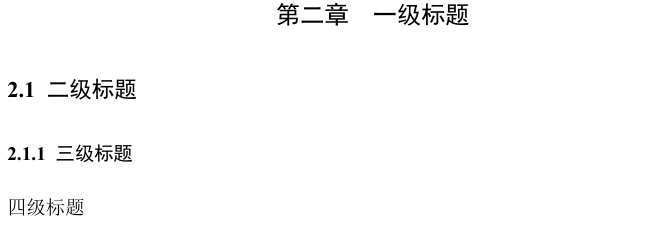
\includegraphics[width=0.5 \linewidth]{figures/2-1}
  \caption{标题格式}
  \label{2:1}
\end{figure}
\section{常用命令}
\subsection{分页}
分页包裹连续分页和奇数页分页,分别对应命令 \verb|\clearpage| 和 \verb|\cleardoublepage|,其中,\verb|\clearpage| 在空白页不会显示页眉页脚
\subsection{文本装饰}
\begin{lstlisting}[caption=文本装饰]
  \CJKunderdot{汉字,下加点} \\
  \CJKunderline{汉字,下划线} \\
  \CJKunderdblline{汉字,双下划线} \\
  \CJKunderwave{汉字,下波浪线} \\
  \CJKsout{汉字,删除线} \\
  \CJKxout{汉字,删除线}
\end{lstlisting}
\begin{center}
  \fbox{
    \parbox{8em}{
      \CJKunderdot{汉字,下加点} \\
      \CJKunderline{汉字,下划线} \\
      \CJKunderdblline{汉字,双下划线} \\
      \CJKunderwave{汉字,下波浪线} \\
      \CJKsout{汉字,删除线} \\
      \CJKxout{汉字,删除线}
    }
  }
\end{center}

\subsection{列表环境}
\LaTeX 提供了三种列表环境:编号的 enumerate 环境,不编号的 itemize 环境和使用关键字的 description 环境。在列表环境内部使用 \verb|\item| 命令开始一个列表项,他可以带一个可选参数表示手动编号或关键字。

enumerate 环境使用数字自动编号:
\clearpage
\begin{lstlisting}[caption=enumerate环境]
  \begin{enumerate}
    \item 中文
    \item English
    \item 日本語
  \end{enumerate}
\end{lstlisting}

\begin{center}
  \fbox{
    \parbox{8em}{
      \begin{enumerate}
        \item 中文
        \item English
        \item 日本語
      \end{enumerate}
    }
  }
\end{center}
itemize 环境不编号,但会在每个条目前加一个符号以示标记:
\begin{lstlisting}[caption=enumerate环境]
  \begin{itemize}
    \item 中文
    \item English
    \item 日本語
  \end{itemize}
\end{lstlisting}

\begin{center}
  \fbox{
    \parbox{8em}{
      \begin{itemize}
        \item 中文
        \item English
        \item 日本語
      \end{itemize}
    }
  }
\end{center}
description 环境总是使用 \verb|\item| 命令的可选参数,把它作为条目关键字加粗显示:
\clearpage
\begin{lstlisting}[caption=enumerate环境]
    \begin{description}
        \item[中文] 中国的语言文学 
        \item[English] The language of England
        \item[日本語] 日本の言語
    \end{description}
\end{lstlisting}

\begin{center}
  \fbox{
    \parbox{14em}{
      \begin{description}
        \item[中文] 中国的语言文学 
        \item[English] The language of England
        \item[日本語] 日本の言語
      \end{description}
    }
  }
\end{center}
这几个环境可以嵌套使用(至多四层),\LaTeX 会自动处理不同层次的缩进和编号。
  \chapter{参考文献}

\section{参考文件格式}
目前本模板仅有 ~{\color{blue}{GB/T~7714-2005}}~和~{\color{blue}{GB/T~7714-2015}}~样式,默认采用~{\color{blue}{GB/T~7714-2015}}~样式,如果需要使用其他格式,请自行寻找或编写 \emph{.bst}文件。

\section{BibTeX 的使用}
模板中有一个\emph{reference.bib}文件,是存放参考文献信息的数据库,通过谷歌学术、微软学术或是百度学术,查找文献时,把其 BibTeX 的引用信息复制到这个文件里,在你需要引用的地方,按照如下方式引用:
\begin{lstlisting}[caption=BibTeX 引用参考文献]
  \cite{bibid}  % bibid 就是你复制引文信息的第一个参数
  \cite{bibid1,bibid2,bibid2}  % 同时引用多个文献
\end{lstlisting}
  

\chapter{数学排版}
\section{行内和行间公式}
数学公式有两种排版方式:其一是与文字混排,称为\textbf{行内公式};其二是单独列为一行排版,称为行间公式。 

行内公式由一对 \texttt\$ 符号包裹:
\begin{lstlisting}
  $a^2 + b^2 = c^2$
\end{lstlisting}
\begin{center}
  \fbox{
    \parbox{10em}{
      \centering $a^2 + b^2 = c^2$
    }
  }
\end{center}
单独成行的行间公式在 \LaTeX{} 里由 equation 环境包裹。equation 环境为公式自动生成一个编号,这个编号可以用 \verb|\label| 和 \verb|\ref| 生成交叉引用,
amsmath 的 \verb|\eqref| 命令甚至为引用自动加上圆括号;还可以用 \verb|\tag| 命令手动修改公式的编号,或者用 \verb|\notag| 命令取消为公式编号。
\begin{lstlisting}[caption=多行公式示例一]
    The Pythagorean theorem is:
    \begin{equation}
      a^2 + b^2 = c^2 \label{pythagorean}
    \end{equation}
    Equation \eqref{pythagorean} is called `Gougu theorem' in Chinese.
\end{lstlisting}
\begin{center}
  \fbox{
    \parbox{30em}{
      The Pythagorean theorem is:
      \begin{equation}
      a^2 + b^2 = c^2 \label{pythagorean}
      \end{equation}
      Equation \eqref{pythagorean} is
      called `Gougu theorem' in Chinese.
    }
  }
\end{center}
\clearpage
\begin{lstlisting}[caption=多行公式示例二]
  It's wrong to say
  \begin{equation}
    1 + 1 = 3 \tag{dumb}
  \end{equation}
  or
  \begin{equation}
    1 + 1 = 4 \notag
  \end{equation}
\end{lstlisting}
\begin{center}
	\fbox{
		\parbox{30em}{
		    It's wrong to say
			\begin{equation}
			1 + 1 = 3 \tag{dumb}
			\end{equation}
			or
			\begin{equation}
			1 + 1 = 4 \notag
			\end{equation}
		}
	}
\end{center}

如果需要直接使用不带编号的行间公式,则将公式用命令 \verb|\[| 和 \verb|\]| 包裹,与之等效的是 \verb|displaymath| 环境。有的人更喜欢 \verb|equation|$*$ 环境,体现了带星号和不带星号的环境之间的区别。

\begin{lstlisting}[caption=多行公式示例三]
  \begin{equation*}
    a^2 + b^2 = c^2
  \end{equation*}
  For short:
  \[ a^2 + b^2 = c^2 \]
  Or if you like the long one:
  \begin{displaymath}
    a^2 + b^2 = c^2
  \end{displaymath}
\end{lstlisting}
\clearpage
\begin{center}
	\fbox{
		\parbox{30em}{
			\begin{equation*}
			a^2 + b^2 = c^2
			\end{equation*}
			For short:
			\[ a^2 + b^2 = c^2 \]
			Or if you like the long one:
			\begin{displaymath}
			a^2 + b^2 = c^2
			\end{displaymath}
		}
	}
\end{center}

我们通过一个例子展示行内公式和行间公式的对比。为了与文字相适应,行内公式在排版大的公式元素(分式、巨算符等)时显得很“局促”:
\begin{lstlisting}[caption=综合示例]
  In text:
  $\lim_{n \to \infty} \sum_{k=1}^n \frac{1}{k^2} = \frac{\pi^2}{6}$.
  In display:
  \[
    \lim_{n \to \infty}
    \sum_{k=1}^n \frac{1}{k^2}
    = \frac{\pi^2}{6}
  \]
\end{lstlisting}
\begin{center}
	\fbox{
		\parbox{30em}{
			In text:
			$\lim_{n \to \infty} \sum_{k=1}^n \frac{1}{k^2} = \frac{\pi^2}{6}$.
			
			In display:
			\[
			  \lim_{n \to \infty}
			  \sum_{k=1}^n \frac{1}{k^2}
			  = \frac{\pi^2}{6}
			\]
		}
	}
\end{center}
\clearpage
\section{数学模式}
当用户使用 \$ 开启行内公式输入,或是使用 \verb|\[| 命令、equation 环境时,\LaTeX{} 就进入了数学模式。数学模式相比于文本模式有以下特点:
\begin{enumerate}
	\item 数学模式中输入的空格被忽略。数学符号的间距默认由符号的性质(关系符号、运算符等)决定。
	需要人为引入间距时,使用 \verb|\quad| 和 \verb|\qquad| 等命令。
	\item 不允许有空行(分段)。行间公式中也无法用 \verb|\\| 命令手动换行。排版多行公式需要用到其他公式环境。
	\item 所有的字母被当作数学公式中的变量处理,字母间距与文本模式不一致,也无法生成单词之间的空格。
\end{enumerate}
\section{数学符号}
\subsection{一般符号}
\begin{table}[htp]
	\centering
	\caption{希腊字母} 
	\begin{quote}\footnotesize%
		\verb|\Alpha|,\verb|\Beta| 等希腊字母符号不存在,因为它们和拉丁字母 A,B 等一模一样;
		小写字母里也不存在 \verb|\omicron|,直接用拉丁字母 $o$ 代替。
	\end{quote}
	\begin{symbols}{*4{cl}}
		\hline
		\SYM{\alpha}     & \SYM{\theta}     & \SYM{o}          & \SYM{\upsilon}  \\
		\SYM{\beta}      & \SYM{\vartheta}  & \SYM{\pi}        & \SYM{\phi}      \\
		\SYM{\gamma}     & \SYM{\iota}      & \SYM{\varpi}     & \SYM{\varphi}   \\
		\SYM{\delta}     & \SYM{\kappa}     & \SYM{\rho}       & \SYM{\chi}      \\
		\SYM{\epsilon}   & \SYM{\lambda}    & \SYM{\varrho}    & \SYM{\psi}      \\
		\SYM{\varepsilon}& \SYM{\mu}        & \SYM{\sigma}     & \SYM{\omega}    \\
		\SYM{\zeta}      & \SYM{\nu}        & \SYM{\varsigma}  &                 \\
		\SYM{\eta}       & \SYM{\xi}        & \SYM{\tau}       &                 \\[1ex]
		\SYM{\Gamma}     & \SYM{\Lambda}    & \SYM{\Sigma}     & \SYM{\Psi}      \\
		\SYM{\Delta}     & \SYM{\Xi}        & \SYM{\Upsilon}   & \SYM{\Omega}    \\
		\SYM{\Theta}     & \SYM{\Pi}        & \SYM{\Phi}       &                 \\[1ex]
		\AMSM{\varGamma} & \AMSM{\varLambda}& \AMSM{\varSigma}  & \AMSM{\varPsi}      \\
		\AMSM{\varDelta} & \AMSM{\varXi}    & \AMSM{\varUpsilon}& \AMSM{\varOmega}    \\
		\AMSM{\varTheta} & \AMSM{\varPi}    & \AMSM{\varPhi}    &                 \\
		\hline
	\end{symbols}
\end{table}
\clearpage
~\\
\begin{table}[H]
	\centering
	\caption{其他符号}
	\begin{symbols}{*4{cl}}
		\hline
		\SYM{\dots}       & \SYM{\cdots}      & \SYM{\vdots}      & \SYM{\ddots}     \\
		\SYM{\hbar}       & \SYM{\imath}      & \SYM{\jmath}      & \SYM{\ell}       \\
		\SYM{\Re}         & \SYM{\Im}         & \SYM{\aleph}      & \SYM{\wp}        \\
		\SYM{\forall}     & \SYM{\exists}     & \LSYM{\mho}       & \SYM{\partial}   \\
		\SYM{'}           & \SYM{\prime}      & \SYM{\emptyset}   & \SYM{\infty}     \\
		\SYM{\nabla}      & \SYM{\triangle}   & \LSYM{\Box}       & \LSYM{\Diamond}  \\
		\SYM{\bot}        & \SYM{\top}        & \SYM{\angle}      & \SYM{\surd}      \\
		\SYM{\diamondsuit} & \SYM{\heartsuit} & \SYM{\clubsuit}   & \SYM{\spadesuit} \\
		\SYM{\neg} or \verb|\lnot| & \SYM{\flat} & \SYM{\natural}    & \SYM{\sharp}     \\
		\hline
	\end{symbols}
\end{table}

\subsection{指数、上下标和导数}
在\LaTeX{}中一般用 $\^$ 和 $\_$ 标明上下标,如果上下标不是一个字符需要使用花括号包裹,否则只对上下标符号后第一个字符起作用。

导数符号 \texttt' (${}'$) 是一类特殊的上标,可以适当连用表示多阶导数,也可以在其后连用上标:
\begin{lstlisting}
  $f(x) = x^2 \quad f'(x) = 2x \quad f''^{2}(x) = 4$
\end{lstlisting}
\begin{center}
	\fbox{
		\parbox{20em}{
			\centering $f(x) = x^2 \quad f'(x) = 2x \quad f''^{2}(x) = 4$
		}
	}
\end{center}
\subsection{分式和根式}
分式使用 \verb|\frac|\{分子\}\{分母\} 来书写。分式的大小在行间公式中是正常大小,而在行内被极度压缩。
\begin{center}
	\fbox{
		\parbox{20em}{
			In display style:
			\[
			3/8 \qquad \frac{3}{8}
			\qquad \tfrac{3}{8}
			\]
			In text style:
			$1\frac{1}{2}$~hours \qquad
			$1\dfrac{1}{2}$~hours
		}
	}
\end{center}
一般的根式使用 \verb|\sqrt{...}|;表示 $n$ 次方根时写成 \verb|\sqrt[n]{...}|.
\begin{center}
	\fbox{
		\parbox{20em}{
			\centering
			$\sqrt{x} \Leftrightarrow x^{1/2}
			\quad \sqrt[3]{2}
			\quad \sqrt{x^{2} + \sqrt{y}}$
		}
	}
\end{center}
特殊的分式形式,如二项式结构,由 amsmath 宏包的 \verb|\binom| 命令生成:
\begin{lstlisting}
  Pascal's rule is
  \[
    \binom{n}{k} =\binom{n-1}{k} + \binom{n-1}{k-1}
  \]
\end{lstlisting}
\begin{center}
	\fbox{
		\parbox{20em}{
			Pascal's rule is
			\[
			\binom{n}{k} =\binom{n-1}{k} + \binom{n-1}{k-1}
			\]
		}
	}
\end{center}
\subsection{关系符}
\LaTeX{}常见的关系符号如下表所示,同时还提供了自定义二元关系符的命令 \verb|\stackrel|,用于将一个符号代价在原有的二元关系符之上:
\begin{lstlisting}
  \[
    f_n(x) \stackrel{*}{\approx} 1
  \]
\end{lstlisting}
\begin{center}
	\fbox{
		\parbox{20em}{
			\centering
			\[
			  f_n(x) \stackrel{*}{\approx} 1
			\]
		}
	}
\end{center}
\clearpage
~\\
\begin{table}[H]
	\centering
	\caption{二元关系符}
	\begin{quote}\footnotesize%
		所有的二元关系符都可以加 \verb|\not| 前缀得到相反意义的关系符,例如 \verb|\not=| 就得到不等号(同 \verb|\ne|)。
	\end{quote}
	\begin{symbols}{*3{cl}}
		\hline
		\SYM{<}              & \SYM{>}                    & \SYM{=}          \\
		\SYM{\leq} or \verb|\le|   & \SYM{\geq} or \verb|\ge| & \SYM{\equiv}     \\
		\SYM{\ll}            & \SYM{\gg}                  & \SYM{\doteq}     \\
		\SYM{\prec}          & \SYM{\succ}                & \SYM{\sim}       \\
		\SYM{\preceq}        & \SYM{\succeq}              & \SYM{\simeq}     \\
		\SYM{\subset}        & \SYM{\supset}              & \SYM{\approx}    \\
		\SYM{\subseteq}      & \SYM{\supseteq}            & \SYM{\cong}      \\
		\LSYM{\sqsubset}     & \LSYM{\sqsupset}           & \LSYM{\Join}     \\
		\SYM{\sqsubseteq}    & \SYM{\sqsupseteq}          & \SYM{\bowtie}    \\
		\SYM{\in}            & \SYM{\ni}, \verb|\owns|      & \SYM{\propto}    \\
		\SYM{\vdash}         & \SYM{\dashv}               & \SYM{\models}    \\
		\SYM{\mid}           & \SYM{\parallel}            & \SYM{\perp}      \\
		\SYM{\smile}         & \SYM{\frown}               & \SYM{\asymp}     \\
		\SYM{:}              & \SYM{\notin}               & \SYM{\neq} or \verb|\ne| \\
		\hline
	\end{symbols}
\end{table}

\begin{table}[H]
	\centering
	\caption{\AmS{} 二元关系符} 
	\begin{symbols}{*3{cl}}
		\hline
		\AMSSYM{\lessdot}           & \AMSSYM{\gtrdot}            & \AMSSYM{\doteqdot} \\
		\AMSSYM{\leqslant}          & \AMSSYM{\geqslant}          & \AMSSYM{\risingdotseq}     \\
		\AMSSYM{\eqslantless}       & \AMSSYM{\eqslantgtr}        & \AMSSYM{\fallingdotseq}    \\
		\AMSSYM{\leqq}              & \AMSSYM{\geqq}              & \AMSSYM{\eqcirc}           \\
		\AMSSYM{\lll} or \verb|\llless| & \AMSSYM{\ggg}               & \AMSSYM{\circeq}  \\
		\AMSSYM{\lesssim}           & \AMSSYM{\gtrsim}            & \AMSSYM{\triangleq}        \\
		\AMSSYM{\lessapprox}        & \AMSSYM{\gtrapprox}         & \AMSSYM{\bumpeq}           \\
		\AMSSYM{\lessgtr}           & \AMSSYM{\gtrless}           & \AMSSYM{\Bumpeq}           \\
		\AMSSYM{\lesseqgtr}         & \AMSSYM{\gtreqless}         & \AMSSYM{\thicksim}         \\
		\AMSSYM{\lesseqqgtr}        & \AMSSYM{\gtreqqless}        & \AMSSYM{\thickapprox}      \\
		\AMSSYM{\preccurlyeq}       & \AMSSYM{\succcurlyeq}       & \AMSSYM{\approxeq}         \\
		\AMSSYM{\curlyeqprec}       & \AMSSYM{\curlyeqsucc}       & \AMSSYM{\backsim}          \\
		\AMSSYM{\precsim}           & \AMSSYM{\succsim}           & \AMSSYM{\backsimeq}        \\
		\AMSSYM{\precapprox}        & \AMSSYM{\succapprox}        & \AMSSYM{\vDash}            \\
		\AMSSYM{\subseteqq}         & \AMSSYM{\supseteqq}         & \AMSSYM{\Vdash}            \\
		\AMSSYM{\shortparallel}     & \AMSSYM{\Supset}            & \AMSSYM{\Vvdash}           \\
		\AMSSYM{\blacktriangleleft} & \AMSSYM{\sqsupset}          & \AMSSYM{\backepsilon}      \\
		\AMSSYM{\vartriangleright}  & \AMSSYM{\because}           & \AMSSYM{\varpropto}        \\
		\AMSSYM{\blacktriangleright}& \AMSSYM{\Subset}            & \AMSSYM{\between}          \\
		\AMSSYM{\trianglerighteq}   & \AMSSYM{\smallfrown}        & \AMSSYM{\pitchfork}        \\
		\AMSSYM{\vartriangleleft}   & \AMSSYM{\shortmid}          & \AMSSYM{\smallsmile}       \\
		\AMSSYM{\trianglelefteq}    & \AMSSYM{\therefore}         & \AMSSYM{\sqsubset}         \\
		\hline
	\end{symbols}
\end{table}
\subsection{算符}
\begin{table}[htp]
	\centering
	\caption{二元运算符}
	\begin{symbols}{*3{cl}}
		\hline
		\SYM{+}              & \SYM{-}              &                     \\
		\SYM{\pm}            & \SYM{\mp}            & \SYM{\triangleleft} \\
		\SYM{\cdot}          & \SYM{\div}           & \SYM{\triangleright}\\
		\SYM{\times}         & \SYM{\setminus}      & \SYM{\star}         \\
		\SYM{\cup}           & \SYM{\cap}           & \SYM{\ast}          \\
		\SYM{\sqcup}         & \SYM{\sqcap}         & \SYM{\circ}         \\
		\SYM{\vee}, \verb|\lor| & \SYM{\wedge},\verb|\land|  & \SYM{\bullet}   \\
		\SYM{\oplus}         & \SYM{\ominus}        & \SYM{\diamond}      \\
		\SYM{\odot}          & \SYM{\oslash}        & \SYM{\uplus}        \\
		\SYM{\otimes}        & \SYM{\bigcirc}       & \SYM{\amalg}        \\
		\SYM{\bigtriangleup} &\SYM{\bigtriangledown}& \SYM{\dagger}       \\
		\LSYM{\lhd}          & \LSYM{\rhd}          & \SYM{\ddagger}      \\
		\LSYM{\unlhd}        & \LSYM{\unrhd}        & \SYM{\wr}           \\
		\hline
	\end{symbols}
\end{table}
\begin{table}[htp]
	\centering
	\caption{\hologo{AmS} 二元运算符} 
	\begin{symbols}{*3{cl}}
		\hline
		\AMSSYM{\dotplus}        & \AMSSYM{\centerdot}      &       \\
		\AMSSYM{\ltimes}         & \AMSSYM{\rtimes}         & \AMSSYM{\divideontimes} \\
		\AMSSYM{\doublecup}      & \AMSSYM{\doublecap}      & \AMSSYM{\smallsetminus} \\
		\AMSSYM{\veebar}         & \AMSSYM{\barwedge}       & \AMSSYM{\doublebarwedge}\\
		\AMSSYM{\boxplus}        & \AMSSYM{\boxminus}       & \AMSSYM{\circleddash}   \\
		\AMSSYM{\boxtimes}       & \AMSSYM{\boxdot}         & \AMSSYM{\circledcirc}   \\
		\AMSSYM{\intercal}       & \AMSSYM{\circledast}     & \AMSSYM{\rightthreetimes} \\
		\AMSSYM{\curlyvee}       & \AMSSYM{\curlywedge}     & \AMSSYM{\leftthreetimes} \\
		\hline
	\end{symbols}
\end{table}
$\nabla$(\verb|\nabla|) 和 $\partial$(\verb|\partial|) 也是常用的算符,虽然它们不属于二元算符。
\LaTeX{} 将数学函数的名称作为一个算符排版,字体为直立字体。
\vspace{2em}
\begin{table}[htp]
	\centering
	\caption{\LaTeX{} 作为算符的函数名称一览}
	\begin{tabular}{*{5}{p{5em}}}
		\hline
		\multicolumn{5}{c}{\textbf{不带上下限的算符}} \\
		\hline
		\verb|\sin| & \verb|\arcsin| & \verb|\sinh| & \verb|\exp| & \verb|\dim| \\
		\verb|\cos| & \verb|\arccos| & \verb|\cosh| & \verb|\log| & \verb|\ker| \\
		\verb|\tan| & \verb|\arctan| & \verb|\tanh| & \verb|\lg|  & \verb|\hom| \\
		\verb|\cot| & \verb|\arg|    & \verb|\coth| & \verb|\ln|  & \verb|\deg| \\
		\verb|\sec| & \verb|\csc|    & \\
		\hline
		\multicolumn{5}{c}{\textbf{带上下限的算符}} \\
		\hline
		\verb|\lim| & \verb|\limsup| & \verb|\liminf| & \verb|\sup| & \verb|\inf| \\
		\verb|\min| & \verb|\max|    & \verb|\det|    & \verb|\Pr|  & \verb|\gcd| \\
		\hline
	\end{tabular}
\end{table}
\clearpage
\begin{lstlisting}
  \[
    \lim_{x \rightarrow 0}
    \frac{\sin x}{x}=1
  \]
\end{lstlisting}
\begin{center}
	\fbox{
		\parbox{20em}{
			\centering
		    \[
			  \lim_{x \rightarrow 0}
			  \frac{\sin x}{x}=1
			\]
		}
	}
\end{center}
对于求模表达式,\LaTeX{} 提供了 \verb|\bmod| 和 \verb|\pmod| 命令,前者相当于一个二元运算符,后者作为同余表达式的后缀:
\begin{lstlisting}
  $a\bmod b \\
  x\equiv a \pmod{b}$
\end{lstlisting}
\begin{center}
	\fbox{
		\parbox{20em}{
		  $a\bmod b \\
		  x\equiv a \pmod{b}$
		}
	}
\end{center}
amsmath 还允许用户在导言区用 \verb|\DeclareMathOperator|定义自己的算符,其中带星号的命令定义带上下限的算符:
\begin{verbatim}
\DeclareMathOperator{\argh}{argh}
\DeclareMathOperator*{\nut}{Nut}
\end{verbatim}
\begin{lstlisting}
  \[\argh 3 = \nut_{x=1} 4x\]
\end{lstlisting}
\begin{center}
	\fbox{
		\parbox{20em}{
			\[\argh 3 = \nut_{x=1} 4x\]
		}
	}
\end{center}
\subsection{巨算符}
积分号 $\int$(\verb|\int|)、求和号 $\sum$ (\verb|\sum|) 等符号称为\textbf{巨算符}。巨算符在行内公式和行间公式的大小和形状有区别。
\begin{lstlisting}
  In text:
  $\sum_{i=1}^n \quad
  \int_0^{\frac{\pi}{2}} \quad
  \oint_0^{\frac{\pi}{2}} \quad
  \prod_\epsilon $ \\
  In display:
  \[\sum_{i=1}^n \quad
  \int_0^{\frac{\pi}{2}} \quad
  \oint_0^{\frac{\pi}{2}} \quad
  \prod_\epsilon \]
\end{lstlisting}
\begin{center}
	\fbox{
		\parbox{20em}{
			In text:
			$\sum_{i=1}^n \quad
			\int_0^{\frac{\pi}{2}} \quad
			\oint_0^{\frac{\pi}{2}} \quad
			\prod_\epsilon $ \\
			In display:
			\[\sum_{i=1}^n \quad
			\int_0^{\frac{\pi}{2}} \quad
			\oint_0^{\frac{\pi}{2}} \quad
			\prod_\epsilon \]
		}
	}
\end{center}
巨算符的上下标位置可由 \verb|\limits| 和 \verb|\nolimits| 调整,前者令巨算符类似 $\lim$ 或求和算符 $\sum$,上下标位于上下方;后者令巨算符类似积分号,上下标位于右上方和右下方。

\begin{lstlisting}
  In text:
  $\sum\limits_{i=1}^n \quad
  \int\limits_0^{\frac{\pi}{2}} \quad
  \prod\limits_\epsilon $ \\
  In display:
  \[\sum\nolimits_{i=1}^n \quad
  \int\limits_0^{\frac{\pi}{2}} \quad
  \prod\nolimits_\epsilon \]
\end{lstlisting}
\begin{center}
	\fbox{
		\parbox{20em}{
			In text:
			$\sum\limits_{i=1}^n \quad
			\int\limits_0^{\frac{\pi}{2}} \quad
			\prod\limits_\epsilon $ \\
			In display:
			\[\sum\nolimits_{i=1}^n \quad
			\int\limits_0^{\frac{\pi}{2}} \quad
			\prod\nolimits_\epsilon \]
		}
	}
\end{center}
amsmath 宏包还提供了 \verb|\substack|,能够在下限位置书写多行表达式;subarray
环境更进一步,令多行表达式可选择居中 (c) 或左对齐 (l):
\begin{lstlisting}
  \[
  \sum_{\substack{0\le i\le n \\
  j\in \mathbb{R}}}
  P(i,j) = Q(n)
  \]
  \[
  \sum_{\begin{subarray}{l}
  0\le i\le n \\
  j\in \mathbb{R}
  \end{subarray}}
  P(i,j) = Q(n)
  \]
\end{lstlisting}
\begin{center}
	\fbox{
		\parbox{20em}{
			\[
			\sum_{\substack{0\le i\le n \\
					j\in \mathbb{R}}}
			P(i,j) = Q(n)
			\]
			\[
			\sum_{\begin{subarray}{l}
				0\le i\le n \\
				j\in \mathbb{R}
				\end{subarray}}
			P(i,j) = Q(n)
			\]
		}
	}
\end{center}
\clearpage
~\\
\begin{table}[H]
	\centering
	\caption{巨算符}
	\def\arraystretch{2.2}
	\begin{symbols}{*3{ccl}}
		\hline
		\BIGSYM{\sum}      & \BIGSYM{\bigcup}   & \BIGSYM{\bigvee}  \\
		\BIGSYM{\prod}     & \BIGSYM{\bigcap}   & \BIGSYM{\bigwedge} \\
		\BIGSYM{\coprod}   & \BIGSYM{\bigsqcup} & \BIGSYM{\biguplus} \\
		\BIGSYM{\int}      & \BIGSYM{\oint}     & \BIGSYM{\bigodot} \\
		\BIGSYM{\bigoplus} & \BIGSYM{\bigotimes} & \\
		\AMSBIG{\iint}     & \AMSBIG{\iiint}    & \AMSBIG{\iiiint}  \\
		\AMSBIG{\idotsint} &                    & \\
		\hline
	\end{symbols}
\end{table}
\subsection{数学重音和上下括号}
\begin{table}[htp]
	\centering
	\caption{数学重音符号}
	\begin{quote}\footnotesize%
		最后一个 \verb|\wideparen| 依赖 yhmath 宏包。
	\end{quote}
	\begin{symbols}{*3{cl}}
		\hline
		\ACC{\hat}{a}   & \ACC{\check}{a} & \ACC{\tilde}{a}       \\
		\ACC{\acute}{a} & \ACC{\grave}{a} & \ACC{\breve}{a}       \\
		\ACC{\bar}{a}   & \ACC{\vec}{a}   & \ACC{\mathring}{a}    \\
		\ACC{\dot}{a}   & \ACC{\ddot}{a}  & \AMSACC{\dddot}{a}    \\
		\AMSACC{\ddddot}{a} \\[1ex]
		\ACC{\widehat}{AAA} & \ACC{\widetilde}{AAA} & \ACC{\wideparen}{AAA} \\
		\hline
	\end{symbols}
\end{table}

\begin{table}[htp]
	\centering
	\caption{作为重音的箭头符号} 
	\begin{symbols}{*2{cl}}
		\hline
		\ACC{\overrightarrow}{AB}     & \AMSACC{\underrightarrow}{AB}     \\
		\ACC{\overleftarrow}{AB}      & \AMSACC{\underleftarrow}{AB}      \\
		\AMSACC{\overleftrightarrow}{AB} & \AMSACC{\underleftrightarrow}{AB} \\
		\hline
	\end{symbols}
\end{table}

\cmd{overbrace} 和 \cmd{underbrace} 命令用来生成上/下括号,各自可带一个上/下标公式。
\begin{lstlisting}
  $\underbrace{\overbrace{(a+b+c)}^6
  \cdot \overbrace{(d+e+f)}^7}
  _\text{meaning of life} = 42$
\end{lstlisting}

\begin{center}
	\fbox{
		\parbox{20em}{
			\centering
			$\underbrace{\overbrace{(a+b+c)}^6
				\cdot \overbrace{(d+e+f)}^7}
			_\text{meaning of life} = 42$
		}
	}
\end{center}

\subsection{箭头}
常用的箭头包括 \cmd{rightarrow} ($\rightarrow$,或 \cmd{to})、\cmd{leftarrow}($\leftarrow$,或 \cmd{gets})等。
\begin{table}[H]
	\centering
	\caption{箭头}
	\begin{symbols}{*2{cl}}
		\hline
		\SYM{\leftarrow} or \cmd{gets} & \SYM{\longleftarrow} \\
		\SYM{\rightarrow} or \cmd{to}   & \SYM{\longrightarrow} \\
		\SYM{\leftrightarrow}    & \SYM{\longleftrightarrow} \\
		\SYM{\Leftarrow}         & \SYM{\Longleftarrow}     \\
		\SYM{\Rightarrow}        & \SYM{\Longrightarrow}    \\
		\SYM{\Leftrightarrow}    & \SYM{\Longleftrightarrow}\\
		\SYM{\mapsto}            & \SYM{\longmapsto}        \\
		\SYM{\hookleftarrow}     & \SYM{\hookrightarrow}    \\
		\SYM{\leftharpoonup}     & \SYM{\rightharpoonup}    \\
		\SYM{\leftharpoondown}   & \SYM{\rightharpoondown}  \\
		\SYM{\rightleftharpoons} & \SYM{\iff}               \\
		\SYM{\uparrow}           & \SYM{\downarrow} \\
		\SYM{\updownarrow}       & \SYM{\Uparrow} \\
		\SYM{\Downarrow}         & \SYM{\Updownarrow} \\
		\SYM{\nearrow}           & \SYM{\searrow} \\
		\SYM{\swarrow}           & \SYM{\nwarrow} \\
		\LSYM{\leadsto}          &              \\
		\hline
	\end{symbols}
\end{table}
amsmath 的 \cmd{xleft\-arrow} 和 \cmd{xright\-arrow} 命令提供了长度可以伸展的箭头,并且可以为箭头增加上下标:
\begin{lstlisting}
  \[ a\xleftarrow{x+y+z} b \]
  \[ c\xrightarrow[x<y]{a*b*c}d \]
\end{lstlisting}
\begin{center}
	\fbox{
		\parbox{20em}{
			 \[ a\xleftarrow{x+y+z} b \]
			\[ c\xrightarrow[x<y]{a*b*c}d \]
		}
	}
\end{center}

\subsection{括号和定界符}

\begin{table}[htp]
	\centering
	\caption{定界符}
	\begin{quote}\footnotesize%
		amsmath 还定义了 \cmd{lvert}、\cmd{rvert} 和 \cmd{lVert}、\cmd{rVert},
		分别作为 \cmd{vert} 和 \cmd{Vert} 对应的开符号(左侧)和闭符号(右侧)的命令。
	\end{quote}
	\begin{symbols}{*4{cl}}
		\hline
		\SYM{(}                  & \SYM{)}                  & \SYM{\uparrow}     & \SYM{\downarrow}   \\
		\SYM{[}  or \cmd{lbrack} & \SYM{]}  or \cmd{rbrack} & \SYM{\Uparrow}     & \SYM{\Downarrow}   \\
		\SYM{\{} or \cmd{lbrace} & \SYM{\}} or \cmd{rbrace} & \SYM{\updownarrow} & \SYM{\Updownarrow} \\
		\SYM{|}  or \cmd{vert}   & \SYM{\|} or \cmd{Vert}   & \SYM{\lceil}       & \SYM{\rceil}       \\
		\SYM{\langle}            & \SYM{\rangle}            & \SYM{\lfloor}      & \SYM{\rfloor}      \\
		\SYM{/}                  & \SYM{\backslash} \\
		\hline
	\end{symbols}
\end{table}

\begin{table}[htp]
	\centering
	\caption{用于行间公式的大定界符}
	\def\arraystretch{1.8}
	\begin{symbols}{*3{cl}}
		\hline
		\DEL{\lgroup}      & \DEL{\rgroup}      & \DEL{\lmoustache}  \\
		\DEL{\arrowvert}   & \DEL{\Arrowvert}   & \DEL{\bracevert} \\
		\DEL{\rmoustache} \\
		\hline
	\end{symbols}
\end{table}

使用 \cmd{left} 和 \cmd{right} 命令可令括号(定界符)的大小可变,在行间公式中常用。\LaTeX{} 会自动根据括号内的公式大小决定定界符大小。
\cmd{left} 和 \cmd{right} 必须成对使用。需要使用单个定界符时,另一个定界符写成 \cmd{left.} 或 \cmd{right.}。

\begin{lstlisting}
  \[1 + \left(\frac{1}{1-x^{2}}
  \right)^3 \qquad
  \left.\frac{\partial f}{\partial t}
  \right|_{t=0}\]
\end{lstlisting}

\begin{center}
	\fbox{
		\parbox{20em}{
			\[1 + \left(\frac{1}{1-x^{2}}
			\right)^3 \qquad
			\left.\frac{\partial f}{\partial t}
			\right|_{t=0}\] 
		}
	}
\end{center}
有时我们不满意于 \LaTeX{} 为我们自动调节的定界符大小。这时我们还可以用 \cmd{big}、\cmd{bigg} 等命令生成固定大小的定界符。
更常用的形式是类似 \cmd{left} 的 \cmd{bigl}、\cmd{biggl} 等,以及类似 \cmd{right} 的 \cmd{bigr}、\cmd{biggr} 等
(\cmd{bigl} 和 \cmd{bigr} 不必成对出现)。
\begin{lstlisting}
  $\Bigl((x+1)(x-1)\Bigr)^{2}$\\
  $\bigl( \Bigl( \biggl( \Biggl( \quad
  \bigr\} \Bigr\} \biggr\} \Biggr\} \quad
  \big\| \Big\| \bigg\| \Bigg\| \quad
  \big\Downarrow \Big\Downarrow
  \bigg\Downarrow \Bigg\Downarrow$
\end{lstlisting}
\begin{center}
	\fbox{
		\parbox{20em}{
			$\Bigl((x+1)(x-1)\Bigr)^{2}$\\
			$\bigl( \Bigl( \biggl( \Biggl( \quad
			\bigr\} \Bigr\} \biggr\} \Biggr\} \quad
			\big\| \Big\| \bigg\| \Bigg\| \quad
			\big\Downarrow \Big\Downarrow
			\bigg\Downarrow \Bigg\Downarrow$
		}
	}
\end{center}

\section{多行公式}
\subsection{长公式折行}
通常来讲应当避免写出超过一行而需要折行的长公式。如果一定要折行的话,习惯上优先在等号之前折行,其次在加号、减号之前,再次在乘号、除号之前。
其它位置应当避免折行。

amsmath 宏包的 multline 环境提供了书写折行长公式的方便环境。
它允许用 \crcmd{} 折行,将公式编号放在最后一行。
多行公式的首行左对齐,末行右对齐,其余行居中。
\begin{lstlisting}
  \begin{multline}
    a + b + c + d + e + f
    + g + h + i \\
    = j + k + l + m + n\\
    = o + p + q + r + s\\
    = t + u + v + x + z
  \end{multline}
\end{lstlisting}
\begin{center}
	\fbox{
		\parbox{20em}{
			\begin{multline}
			a + b + c + d + e + f
			+ g + h + i \\
			= j + k + l + m + n\\
			= o + p + q + r + s\\
			= t + u + v + x + z 
			\end{multline}
		}
	}
\end{center}

\subsection{多行公式}
更多的情况是,我们需要罗列一系列公式,并令其按照等号对齐。目前最常用的是 align 环境,它将公式用 \texttt\& 隔为两部分并对齐。分隔符通常放在等号左边:
\begin{lstlisting}
  \begin{align}
    a & = b + c \\
      & = d + e
  \end{align}
\end{lstlisting}
\begin{center}
	\fbox{
		\parbox{20em}{
			\begin{align}
			a & = b + c \\
			& = d + e
			\end{align}
		}
	}
\end{center}
align 环境会给每行公式都编号。我们仍然可以用 \cmd{notag} 去掉某行的编号。
在以下的例子,为了对齐等号,我们将分隔符放在右侧,并且此时需要在等号后添加一对括号 \texttt\{\texttt\} 以产生正常的间距:
\begin{lstlisting}
  \begin{align}
  a ={} & b + c \\
  ={} & d + e + f + g + h + i
  + j + k + l \notag \\
  & + m + n + o \\
  ={} & p + q + r + s
  \end{align}
\end{lstlisting}
\begin{center}
	\fbox{
		\parbox{20em}{
			\begin{align}
			a ={} & b + c \\
			={} & d + e + f + g + h + i
			+ j + k + l \notag \\
			& + m + n + o \\
			={} & p + q + r + s
			\end{align}
		}
	}
\end{center}
align 还能够对齐多组公式,除等号前的 \texttt\& 之外,公式之间也用 \texttt\& 分隔:
\begin{lstlisting}
  \begin{align}
  a &=1  &  b &=2   & c &=3   \\
  d &=-1 &  e &=-2  & f &=-5
  \end{align}
\end{lstlisting}
\begin{center}
	\fbox{
		\parbox{20em}{
			\begin{align}
			a &=1  &  b &=2   & c &=3   \\
			d &=-1 &  e &=-2  & f &=-5
			\end{align}
		}
	}
\end{center}
如果我们不需要按等号对齐,只需罗列数个公式,gather 将是一个很好用的环境:
\begin{lstlisting}
\begin{gather}
a = b + c \\
d = e + f + g \\
h + i = j + k \notag \\
l + m = n
\end{gather}
\end{lstlisting}
\begin{center}
	\fbox{
		\parbox{20em}{
			\begin{gather}
			a = b + c \\
			d = e + f + g \\
			h + i = j + k \notag \\
			l + m = n
			\end{gather}
		}
	}
\end{center}
\subsection{公用编号的多行公式}
另一个常见的需求是将多个公式组在一起公用一个编号,编号位于公式的居中位置。为此,amsmath 宏包
提供了诸如 aligned、gathered 等环境,与 equation 环境套用。
以 \texttt{-ed} 结尾的环境用法与前一节不以 \texttt{-ed} 结尾的环境用法一一对应。我们仅以 aligned 举例:
\begin{lstlisting}
  \begin{equation}
	  \begin{aligned}
		  a &= b + c \\
		  d &= e + f + g \\
		  h + i &= j + k \\
		  l + m &= n
	  \end{aligned}
  \end{equation}
\end{lstlisting}
\begin{center}
	\fbox{
		\parbox{20em}{
			\begin{equation}
				\begin{aligned}
					a &= b + c \\
					d &= e + f + g \\
					h + i &= j + k \\
					l + m &= n
				\end{aligned}
			\end{equation}
		}
	}
\end{center}
\section{数组和矩阵}
为了排版二维数组,\LaTeX{} 提供了 \env{array} 环境,用法与 \env{tabular} 环境极为类似,也需要定义列格式,并用 \crcmd{} 换行。
数组可作为一个公式块,在外套用 \cmd{left}、\cmd{right} 等定界符:

\begin{lstlisting}
  \[ \mathbf{X} = \left(
    \begin{array}{cccc}
    x_{11} & x_{12} & \ldots & x_{1n}\\
    x_{21} & x_{22} & \ldots & x_{2n}\\
    \vdots & \vdots & \ddots & \vdots\\
    x_{n1} & x_{n2} & \ldots & x_{nn}\\
    \end{array} 
  \right) \]
\end{lstlisting}
\begin{center}
	\fbox{
		\parbox{25em}{
			\[ \mathbf{X} = \left(
			\begin{array}{cccc}
			x_{11} & x_{12} & \ldots & x_{1n}\\
			x_{21} & x_{22} & \ldots & x_{2n}\\
			\vdots & \vdots & \ddots & \vdots\\
			x_{n1} & x_{n2} & \ldots & x_{nn}\\
			\end{array} 
			\right) \]
		}
	}
\end{center}
我们还可以利用空的定界符排版出这样的效果:
\begin{lstlisting}
  \[ |x| = \left\{
    \begin{array}{rl}
      -x & \text{if } x < 0,\\
      0 & \text{if } x = 0,\\
      x & \text{if } x > 0.
    \end{array} \right. 
  \]
\end{lstlisting}
\begin{center}
	\fbox{
		\parbox{25em}{
			\[ |x| = \left\{
			\begin{array}{rl}
			-x & \text{if } x < 0,\\
			0 & \text{if } x = 0,\\
			x & \text{if } x > 0.
			\end{array} \right. 
			\]
		}
	}
\end{center}
不过上述例子可以用 amsmath 提供的 \env{cases} 环境更轻松地完成:
\begin{lstlisting}
  \[ |x| =
    \begin{cases}
      -x & \text{if } x < 0,\\
      0 & \text{if } x = 0,\\
      x & \text{if } x > 0.
    \end{cases} 
  \]
\end{lstlisting}
\begin{center}
	\fbox{
		\parbox{25em}{
			  \[ |x| =
			\begin{cases}
			-x & \text{if } x < 0,\\
			0 & \text{if } x = 0,\\
			x & \text{if } x > 0.
			\end{cases} 
			\]
		}
	}
\end{center}
我们当然也可以用 \env{array} 环境排版各种矩阵。amsmath 宏包还直接提供了多种排版矩阵的环境,包括不带定界符的 \env{matrix},
以及带各种定界符的矩阵 \env{pmatrix}($\bigl($)、\env{bmatrix}($\bigl[$)、\env{Bmatrix}($\bigl\{$)、
\env{vmatrix}($\bigl\vert$)、\env{Vmatrix}($\bigl\Vert$)。使用这些环境时,无需给定列格式:
\begin{lstlisting}
  \[
  \begin{matrix}
  1 & 2 \\ 3 & 4
  \end{matrix} \qquad
  \begin{bmatrix}
  x_{11} & x_{12} & \ldots & x_{1n}\\
  x_{21} & x_{22} & \ldots & x_{2n}\\
  \vdots & \vdots & \ddots & \vdots\\
  x_{n1} & x_{n2} & \ldots & x_{nn}\\
  \end{bmatrix}
  \]
\end{lstlisting}
\begin{center}
	\fbox{
		\parbox{25em}{
			  \[
			\begin{matrix}
			1 & 2 \\ 3 & 4
			\end{matrix} \qquad
			\begin{bmatrix}
			x_{11} & x_{12} & \ldots & x_{1n}\\
			x_{21} & x_{22} & \ldots & x_{2n}\\
			\vdots & \vdots & \ddots & \vdots\\
			x_{n1} & x_{n2} & \ldots & x_{nn}\\
			\end{bmatrix}
			\]
		}
	}
\end{center}
\section{公式中的间距}
绝大部分时候,数学公式中各元素的间距是根据符号类型自动生成的,需要我们手动调整的情况极少。
我们已经认识了两个生成间距的命令 \cmd{quad} 和 \cmd{qquad}。在公式中我们还可能用到的间距包括 \cmd{,}、\cmd{:}、\cmd{;}
以及负间距 \cmd{!},其中 \cmd{quad} 、 \cmd{qquad} 和 \cmd{,} 在文本和数学环境中可用,后三个命令只用于数学环境。
文本中的 \cmd{\textvisiblespace} 也能使用在数学公式中。

\newdimen\testdimen \testdimen=\fontdimen6\textfont2 \divide\testdimen18\relax
\begin{center}
	\begin{tabularx}{0.9\textwidth}{*{3}{>{\raggedright\arraybackslash}X}|*{3}{>{\raggedright\arraybackslash}X}}
		\hline
		无额外间距  &                          & $a a$        &
		\cmd{,}     & \demowidth{3\testdimen}  & $a\,a$       \\
		\cmd{quad}  & \demowidth{18\testdimen} & $a\quad a$   &
		\cmd{:}     & \demowidth{4\testdimen}  & $a\:a$       \\
		\cmd{qquad} & \demowidth{36\testdimen} & $a\qquad a$  &
		\cmd{;}     & \demowidth{5\testdimen}  & $a\;a$       \\
		\cmd{\textvisiblespace}     & \demowidth{\fontdimen2\textfont0} & $a\ a$ &
		\cmd{!}     & $-$\demowidth{3\testdimen} & $a\!a$     \\
		\hline
	\end{tabularx}
\end{center}
一个常见的用途是修正积分的被积函数$f(x)$和微元$\mathrm{d}x$之间的距离。注意微元里的$\mathrm{d}$用的是直立体:
\begin{lstlisting}
  \[
  \int_a^b f(x)\mathrm{d}x
  \qquad
  \int_a^b f(x)\,\mathrm{d}x
  \]
\end{lstlisting}
\begin{center}
	\fbox{
		\parbox{20em}{
			  \[
			\int_a^b f(x)\mathrm{d}x
			\qquad
			\int_a^b f(x)\,\mathrm{d}x
			\]
		}
	}
\end{center}

\section{数学符号的字体控制}
\subsection{数学字母字体}
\LaTeX{} 允许一部分数学符号切换字体,主要是拉丁字母、数字、大写希腊字母以及重音符号等。
表 \ref{tbl:math-fonts} 给出了切换字体的命令。某一些命令需要字体宏包的支持。
\begin{table}[htp]
	\centering
	\caption{数学字母字体} \label{tbl:math-fonts}
	\begin{tabular}{*{3}{l}}
		\hline
		\textbf{示例}    & \textbf{命令} & \textbf{依赖的宏包}\\
		\hline
		$\mathnormal{ABCDE abcde 1234}$  & \cmd{mathnormal}\marg*{\ldots}&       \\
		$\mathrm{ABCDE abcde 1234}$      & \cmd{mathrm}\marg*{\ldots}    &       \\
		$\mathit{ABCDE abcde 1234}$      & \cmd{mathit}\marg*{\ldots}    &       \\
		$\mathbf{ABCDE abcde 1234}$      & \cmd{mathbf}\marg*{\ldots}    &       \\
		$\mathsf{ABCDE abcde 1234}$      & \cmd{mathsf}\marg*{\ldots}    &       \\
		$\mathtt{ABCDE abcde 1234}$      & \cmd{mathtt}\marg*{\ldots}    &       \\
		$\CMcal{ABCDE}$                  & \cmd{mathcal}\marg*{\ldots}   & 仅提供大写字母 \\
		\hline
		$\EuScript{ABCDE}$               & \cmd{mathcal}\marg*{\ldots}   & eucal 仅提供大写字母 \\
		$\mathscr{ABCDE}$                & \cmd{mathscr}\marg*{\ldots}   & mathrsfs 仅提供大写字母\\
		$\mathfrak{ABCDE abcde 1234}$    & \cmd{mathfrak}\marg*{\ldots}  & amssymb 或 eufrak  \\
		$\mathbb{ABCDE}$                 & \cmd{mathbb}\marg*{\ldots}    & amssymb 仅提供大写字母 \\
		\hline
	\end{tabular}
\end{table}

\subsection{数学符号的尺寸}
数学符号按照符号排版的位置规定尺寸,从大到小包括行间公式尺寸、行内公式尺寸、上下标尺寸、次级上下标尺寸。
除了字号有别之外,行间和行内公式尺寸下的巨算符也使用不一样的大小。\LaTeX{} 为每个数学尺寸指定了一个切换的命令,见表 \ref{tbl:math-size}。

\begin{table}[htp]
	\centering
	\caption{数学符号尺寸}\label{tbl:math-size}
	\begin{tabular}{lll}
		\hline
		\textbf{命令} & \textbf{尺寸} & \textbf{示例} \\
		\hline
		\cmd{displaystyle}      & 行间公式尺寸   & $\displaystyle\sum a $\\
		\cmd{textstyle}         & 行内公式尺寸   & $\textstyle\sum a $ \\
		\cmd{scriptstyle}       & 上下标尺寸     & $\scriptstyle a$ \\
		\cmd{scriptscriptstyle} & 次级上下标尺寸 & $\scriptscriptstyle a$\\
		\hline
	\end{tabular}
\end{table}
我们通过以下示例对比行间公式和行内公式的区别。在分式中,分子分母默认为行内公式尺寸,示例中将分母切换到行间公式尺寸:
\clearpage
\begin{lstlisting}
  \[
    r = \frac
    {\sum_{i=1}^n (x_i- x)(y_i- y)}
    {\displaystyle \left[
    \sum_{i=1}^n (x_i-x)^2
    \sum_{i=1}^n (y_i-y)^2
    \right]^{1/2} }
  \]
\end{lstlisting}
\begin{center}
	\fbox{
		\parbox{20em}{
			\[
			r = \frac
			{\sum_{i=1}^n (x_i- x)(y_i- y)}
			{\displaystyle \left[
				\sum_{i=1}^n (x_i-x)^2
				\sum_{i=1}^n (y_i-y)^2
				\right]^{1/2} }
			\]
		}
	}
\end{center}



















  \chapter{插入图片}
\section{基本使用}
\LaTeX{} 本身不支持插图功能,需要由 \pkg{graphicx} 宏包辅助支持。
在调用了 \pkg{graphicx} 宏包以后,就可以使用 \cmd{include\-graphics} 命令加载图片了:
\begin{lstlisting}
	\includegraphics[<options>]{<filename>}
\end{lstlisting}
其中 \Arg{filename} 为图片文件名,与 \cmd{include} 命令的用法类似,文件名可能需要用相对路径或绝对路径表示。图片文件的扩展名一般可不写。另外一定要注意,\textbf{文件名里既不要有空格(类似 \cmd{include}),也不要有多余的英文点号},否则宏包在解析文件名的过程中会出错。

另外 \pkg{graphicx} 宏包还提供了 \cmd{graphics\-path} 命令,用于声明一个或多个图片文件存放的目录,
使用这些目录里的图片时可不用写路径:
\begin{lstlisting}
  % 假设主要的图片放在 figures 子目录下,标志放在 logo 子目录下
  \graphicspath{{figures/}{logo/}}
\end{lstlisting}

\cmd{includegraphics} 命令的可选参数 \Arg{options} 支持 \Arg{key}=\Arg{value} 形式赋值,常用的参数如下:
\begin{table}[htp]
	\centering
	\caption{\cmd{includegraphics} 命令的可选参数}\label{tbl:graphics-options}
	\begin{tabular}{lp{18em}}
		\hline
		\textbf{参数} & \textbf{含义} \\
		\hline
		\texttt{width=}\Arg{width}    &  将图片缩放到宽度为 \Arg{width} \\
		\texttt{height=}\Arg{height}  &  将图片缩放到高度为 \Arg{height} \\
		\texttt{scale=}\Arg{scale}    &  将图片相对于原尺寸缩放 \Arg{scale} 倍 \\
		\texttt{angle=}\Arg{angle}    &  令图片逆时针旋转 \Arg{angle} 度 \\
		\hline
	\end{tabular}
\end{table}
\clearpage
\section{排版多行多列图片}
这里给个离职,模仿写就好:
\begin{lstlisting}
  \begin{figure}[htbp]
    \centering
    \includegraphics[width=...]{...}
    \qquad
    \includegraphics[width=...]{...} \\[..pt]
    \includegraphics[width=...]{...}
    \caption{...}
    \label{...}
  \end{figure}
\end{lstlisting}
\begin{figure}[htp]
	\centering
	\fcolorbox[gray]{0}{0.96}{\parbox{10em}{\vrule width 0pt height 10ex\hfil}}
	\qquad
	\fcolorbox[gray]{0}{0.96}{\parbox{10em}{\vrule width 0pt height 12ex\hfil}}
	\par\bigskip
	\fcolorbox[gray]{0}{0.96}{\parbox{20em}{\vrule width 0pt height 12ex\hfil}}
	\caption{并排放置图片的示意。}\label{fig:parallel-fig}
\end{figure}
或者使用这种方式,个人比较喜欢下面这种:
\clearpage
\begin{lstlisting}
  \begin{figure}[t]
    \centering
    \subfloat[图1]{
      \label{fig1}
      \includegraphics[width=0.5\textwidth]{图1}
    }
    \subfloat[图2]{
      \label{fig2}
      \includegraphics[width=0.5\textwidth]{图2}
    }\\ 
    \subfloat[图3]{
      \label{fig3}
      \includegraphics[width=0.5\textwidth]{图3}
    } 
    \subfloat[图4]{
      \label{fig4}
      \includegraphics[width=0.5\textwidth]{图4}
    }
    \caption{多行多列子图}
    \label{fig}	
  \end{figure}
\end{lstlisting}
\begin{figure}[H]
	\centering
	\subfloat[图1]{
		\label{fig1}
		\fcolorbox[gray]{0}{0.96}{\parbox{10em}{\vrule width 0pt height 10ex\hfil}}
	}% 
	\subfloat[图2]{
		\label{fig2}
		\fcolorbox[gray]{0}{0.96}{\parbox{10em}{\vrule width 0pt height 10ex\hfil}}
	}\\ 
	\subfloat[图3]{
		\label{fig3}
		\fcolorbox[gray]{0}{0.96}{\parbox{10em}{\vrule width 0pt height 10ex\hfil}}
	} 
	\subfloat[图4]{
		\label{fig4}
		\fcolorbox[gray]{0}{0.96}{\parbox{10em}{\vrule width 0pt height 10ex\hfil}}
	}
	\caption{多行多列子图}
	\label{fig}	
\end{figure}
  \chapter{插入表格}
\LaTeX{} 里排版表格不如 Word 等所见即所得的工具简便和自由,不过对于不太复杂的表格来讲,完全能够胜任。

排版表格最基本的 \env{tabular} 环境用法为:
\begin{lstlisting}
  \begin{tabular}[align]{column-spec}
    <item1> & <item2> & ... \\
    \hline
    <item1> & <item2> & ... \\
  \end{tabular}
\end{lstlisting}
其中 \Arg{column-spec} 是列格式标记,在接下来的内容将仔细介绍;\texttt\& 用来分隔单元格;
\crcmd{} 用来换行;\cmd{hline} 用来在行与行之间绘制横线。


直接使用 \env{tabular} 环境的话,会\textbf{和周围的文字混排}。此时可用一个可选参数 \Arg{align} 控制垂直对齐:
\verb|t| 和 \verb|b| 分别表示按表格顶部、底部对齐,其他参数或省略不写(默认)表示居中对齐。
\begin{lstlisting}
  \begin{tabular}{|c|}
  center-\\ aligned \\
  \end{tabular},
  
  \begin{tabular}[t]{|c|}
  top-\\ aligned \\
  \end{tabular},
  
  \begin{tabular}[b]{|c|}
  bottom-\\ aligned\\
  \end{tabular} tabulars.
\end{lstlisting}
\begin{center}
	\fbox{
		\parbox{30em}{
			\centering
			\begin{tabular}{|c|}
				center-\\ aligned \\
			\end{tabular},
			\begin{tabular}[t]{|c|}
				top-\\ aligned \\
			\end{tabular},
			\begin{tabular}[b]{|c|}
				bottom-\\ aligned\\
			\end{tabular} tabulars.
		}
	}
\end{center}

但是通常情况下 \env{tabular} 环境很少与文字直接混排,而是会放在 \env{table} 浮动体环境中,并用 \cmd{caption} 命令加标题。

\section{列格式}
\env{tabular} 环境使用 \Arg{column-spec} 参数指定表格的列数以及每列的格式。
\begin{table}[htp]
	\centering
	\caption{\LaTeX{} 表格列格式}
	\begin{tabular}{*{2}{l}}
		\hline
		\textbf{列格式} & \textbf{说明} \\
		\hline
		\ttfamily l/c/r          & 单元格内容左对齐/居中/右对齐,不折行 \\
		\ttfamily p\marg{width}  & 单元格宽度固定为 \Arg{width},可自动折行 \\
		\ttfamily |              & 绘制竖线 \\
		\ttfamily @\marg{string} & 自定义内容 \Arg{string} \\
		\hline
	\end{tabular}
\end{table}

\begin{lstlisting}
  \begin{tabular}{lcr|p{6em}}
    \hline
    left & center & right
    & par box with fixed width\\
    L & C & R & P \\
    \hline
  \end{tabular}
\end{lstlisting}
\begin{center}
	\fbox{
		\parbox{20em}{
			\centering
			\begin{tabular}{lcr|p{6em}}
				\hline
				left & center & right
				& par box with fixed width\\
				L    & C      & R     & P \\
				\hline
			\end{tabular}
		}
	}
\end{center}

表格中每行的单元格数目不能多于列格式里 \texttt{l/c/r/p} 的总数(可以少于这个总数),否则出错。

\texttt{@} 格式可在单元格前后插入任意的文本,但同时它也消除了单元格前后额外添加的间距。
\texttt{@} 格式可以适当使用以充当“竖线”。特别地,\texttt{@}\marg*{} 可直接用来消除单元格前后的间距:
\clearpage
\begin{lstlisting}
  \begin{tabular}{@{} r@{:}lr @{}}
    \hline
    1  & 1 & one \\
    11 & 3 & eleven \\
    \hline
  \end{tabular}
\end{lstlisting}
\begin{center}
	\fbox{
		\parbox{20em}{
			\centering
			\begin{tabular}{@{} r@{:}lr @{}}
				\hline
				1  & 1 & one \\
				11 & 3 & eleven \\
				\hline
			\end{tabular}
		}
	}
\end{center}
另外 \LaTeX{} 还提供了简便的将格式参数重复的写法 \texttt*\marg{n}\marg{column-spec},比如以下两种写法是等效的:
\begin{verbatim}
\begin{tabular}{|c|c|c|c|c|p{4em}|p{4em}|}
\begin{tabular}{|*{5}{c|}*{2}{p{4em}|}}
\end{verbatim}
有时需要为整列修饰格式,比如整列改变为粗体,如果每个单元格都加上 \cmd{bfseries} 命令会比较麻烦。
\pkg{array} 宏包提供了辅助格式 \texttt> 和 \texttt<,用于给列格式前后加上修饰命令:

\begin{lstlisting}
  % \usepackage{array}
  \begin{tabular}{>{\itshape}r<{*}l}
    \hline
    italic & normal \\
    column & column \\
    \hline
  \end{tabular}
\end{lstlisting}
\begin{center}
	\fbox{
		\parbox{20em}{
			\centering
			\begin{tabular}{>{\itshape}r<{*}l}
				\hline
				italic & normal \\
				column & column \\
				\hline
			\end{tabular}
			
		}
	}
\end{center}

辅助格式甚至支持插入 \cmd{centering} 等命令改变 \texttt{p} 列格式的对齐方式,
一般还要加额外的命令 \cmd{array\-back\-slash} 以免出错。


\begin{lstlisting}
  % \usepackage{array}
  \begin{tabular}{>{\centering\arraybackslash}p{9em}}
    \hline
    Some center-aligned long text. \\
    \hline
  \end{tabular}
\end{lstlisting}

\begin{center}
	\fbox{
		\parbox{20em}{
			\centering
			\begin{tabular}{>{\centering\arraybackslash}p{9em}}
				\hline
				Some center-aligned long text. \\
				\hline
			\end{tabular}
		}
	}
\end{center}

\pkg{array} 宏包还提供了类似 \texttt{p} 格式的 \texttt{m} 格式和 \texttt{b} 格式,
三者分别在垂直方向上靠顶端对齐、居中以及底端对齐。
\begin{lstlisting}
  % \usepackage{array}
  \newcommand\txt{a b c d e f g h i}
  \begin{tabular}{cp{2em}m{2em}b{2em}}
    \hline
    pos & \txt & \txt & \txt \\
    \hline
  \end{tabular}
\end{lstlisting}
\begin{center}
	\fbox{
		\parbox{20em}{
			\centering
			\newcommand\txt{a b c d e f g h i}
			\begin{tabular}{cp{2em}m{2em}b{2em}}
				\hline
				pos & \txt & \txt & \txt \\
				\hline
			\end{tabular}
		}
	}
\end{center}
\clearpage
\section{列宽}
在控制列宽方面,\LaTeX{} 表格有着明显的不足:\texttt{l/c/r} 格式的列宽是由文字内容的自然宽度决定的,
而 \texttt{p} 格式给定了列宽却不好控制对齐(可用 \pkg{array} 宏包的辅助格式),
更何况列与列之间通常还有间距,所以直接生成给定总宽度的表格并不容易。

\pkg{tabularx} 宏包为我们提供了方便的解决方案。它引入了一个 \texttt{X} 列格式,类似 \texttt{p} 列格式,
不过会根据表格宽度自动计算列宽,多个 \texttt{X} 列格式平均分配列宽。
\texttt{X} 列格式也可以用 \pkg{array} 里的辅助格式修饰对齐方式:
\begin{lstlisting}
  % \usepackage{array,tabularx}
  \begin{tabularx}{14em}{|*{4}{>{\centering\arraybackslash}X|}}
    \hline
    A & B & C & D \\ \hline
    a & b & c & d \\ \hline
  \end{tabularx}
\end{lstlisting}
\begin{center}
	\fbox{
		\parbox{20em}{
			\centering
			\begin{tabularx}{14em}%
				{|*{4}{>{\centering\arraybackslash}X|}}
				\hline
				A & B & C & D \\ \hline
				a & b & c & d \\ \hline
			\end{tabularx}
		}
	}
\end{center}

\section{横线}

我们已经在之前的例子见过许多次绘制表格线的 \cmd{hline} 命令。另外 \cmd{cline}\marg*{\Arg{i}-\Arg{j}} 用来绘制跨越部分单元格的横线:
\begin{lstlisting}
  \begin{tabular}{|c|c|c|}
    \hline
    4 & 9 & 2 \\ \cline{2-3}
    3 & 5 & 7 \\ \cline{1-1}
    8 & 1 & 6 \\ \hline
  \end{tabular}
\end{lstlisting}

\begin{center}
	\fbox{
		\parbox{20em}{
			\centering
			\begin{tabular}{|c|c|c|}
				\hline
				4 & 9 & 2 \\ \cline{2-3}
				3 & 5 & 7 \\ \cline{1-1}
				8 & 1 & 6 \\ \hline
			\end{tabular}
		}
	}
\end{center}

在科技论文排版中广泛应用的表格形式是三线表,形式干净简明。
三线表由 \pkg{booktabs} 宏包支持,它提供了 \cmd{toprule}、\cmd{midrule} 和 \cmd{bottomrule} 命令用以排版三线表的三条线,以及和 \cmd{cline} 对应的 \cmd{cmidrule}。除此之外,最好不要用其它横线以及竖线:
\begin{lstlisting}
  % \usepackage{booktabs}
  \begin{tabular}{cccc}
    \toprule
    & \multicolumn{3}{c}{Numbers} \\
    \cmidrule{2-4}
    & 1 & 2 & 3 \\
    \midrule
    Alphabet & A & B & C \\
    Roman    & I & II& III \\
    \bottomrule
  \end{tabular}
\end{lstlisting}

\begin{center}
	\fbox{
		\parbox{20em}{
			\centering
			\begin{tabular}{cccc}
				\toprule
				& \multicolumn{3}{c}{Numbers} \\
				\cmidrule{2-4}
				& 1 & 2 & 3 \\
				\midrule
				Alphabet & A & B & C \\
				Roman    & I & II& III \\
				\bottomrule
			\end{tabular}
		}
	}
\end{center}
\section{合并单元格}
\LaTeX{} 是一行一行排版表格的,横向合并单元格较为容易,由 \cmd{multi\-column} 命令实现:
\begin{lstlisting}
  \multicolumn{<n>}{<column-spec>}{<item>}
\end{lstlisting}
其中 \Arg{n} 为要合并的列数,\Arg{column-spec} 为合并单元格后的列格式,只允许出现一个 \texttt{l/c/r} 或 \texttt{p} 格式。
如果合并前的单元格前后带表格线 \texttt|,合并后的列格式也要带 \texttt| 以使得表格的竖线一致。
\begin{lstlisting}
  \begin{tabular}{|c|c|c|}
    \hline
    1 & 2 & Center \\ \hline
    \multicolumn{2}{|c|}{3} & \multicolumn{1}{r|}{Right} \\ 
    \hline
    4 & \multicolumn{2}{c|}{C} \\ 
    \hline
  \end{tabular}
\end{lstlisting}
\begin{center}
	\fbox{
		\parbox{20em}{
			\centering
			\begin{tabular}{|c|c|c|}
				\hline
				1 & 2 & Center \\ \hline
				\multicolumn{2}{|c|}{3} &
				\multicolumn{1}{r|}{Right} \\ \hline
				4 & \multicolumn{2}{c|}{C} \\ \hline
			\end{tabular}
		}
	}
\end{center}

上面的例子还体现了,形如 \cmd{multicolumn}\marg*{1}\marg{column-spec}\marg{item} 的命令{\bf 可以用来修改某一个单元格的列格式。}

纵向合并单元格需要用到 \pkg{multirow} 宏包提供的 \cmd{multirow} 命令:
\begin{lstlisting}
	\multirow{<n>}{<width>}{<item>}
\end{lstlisting}
\Arg{width} 为合并后单元格的宽度,可以填 \texttt{*} 以使用自然宽度。

我们看一个结合 \cmd{cline}、\cmd{multi\-column} 和 \cmd{multi\-row} 命令的例子:

\begin{lstlisting}
  % \usepackage{multirow}
  \begin{tabular}{ccc}
    \hline
    \multirow{2}{*}{Item} & \multicolumn{2}{c}{Value} \\ \cline{2-3}
    & First & Second  \\ \hline
    A & 1 & 2 \\  \hline
  \end{tabular}
\end{lstlisting}
\begin{center}
	\fbox{
		\parbox{20em}{
			\centering
			\begin{tabular}{ccc}
				\hline
				\multirow{2}{*}{Item} & \multicolumn{2}{c}{Value} \\
				\cline{2-3}
				& First & Second 
				\\ \hline
				A & 1     & 2 \\ 
				\hline
			\end{tabular}
		}
	}
\end{center}


\section{行距控制}
\LaTeX{} 生成的表格看起来通常比较紧凑。修改参数 \cmd{array\-stretch} 可以得到行距更加宽松的表格:
\begin{lstlisting}
  \renewcommand\arraystretch{1.8}
  \begin{tabular}{|c|}
    \hline
    Really loose \\ \hline
    tabular rows.\\ \hline
  \end{tabular}
\end{lstlisting}
\begin{center}
	\fbox{
		\parbox{20em}{
			\centering
			\renewcommand\arraystretch{1.8}
			\begin{tabular}{|c|}
				\hline
				Really loose \\ \hline
				tabular rows.\\ \hline
			\end{tabular}
		}
	}
\end{center}

另一种增加间距的办法是给换行命令 \crcmd{} 添加可选参数,在这一行下面加额外的间距,适合用于在行间不加横线的表格:
\begin{lstlisting}
  \begin{tabular}{c}
    \hline
    Head lines \\[6pt]
    tabular lines \\
    tabular lines \\ \hline
  \end{tabular}
\end{lstlisting}
\begin{center}
	\fbox{
		\parbox{20em}{
			\centering
			\begin{tabular}{c}
				\hline
				Head lines \\[6pt]
				tabular lines \\
				tabular lines \\ \hline
			\end{tabular}
		}
	}
\end{center}

但是这种换行方式的存在导致了一个缺陷——{\bf{表格的首个单元格不能直接使用中括号 \text{[~]}}},
否则 \crcmd{} 往往会将下一行的中括号当作自己的可选参数,因而出错。如果要使用中括号,应当放在花括号 \marg*{} 里面。
或者也可以选择将换行命令写成 \crcmd\texttt{[0pt]}。

































  \chapter{插入算法}
  \chapter{自定义宏}
  
  % 致谢
  \addthanks{
	本模板编写参考了《 \LaTeX{} 入门》\cite{刘海洋2013LATEX},《简单高效 \LaTeX 》和 《\LaTeX{} 范例学习与试卷论文排版》等。
}

  
  % 参考文献开始
  \addreference
\end{lstlisting}
在正文内部,可以分四个层级,例如:
\begin{lstlisting}[caption=章节命令使用]
  \chapter{一级标题}
  \section{二级标题}
  \subsection{三级标题}
  \subsubsection{四级标题}
\end{lstlisting}
\begin{figure}[H]
  \centering 
  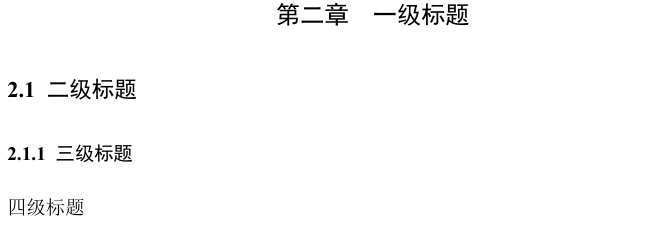
\includegraphics[width=0.5 \linewidth]{figures/2-1}
  \caption{标题格式}
  \label{2:1}
\end{figure}
\section{常用命令}
\subsection{分页}
分页包裹连续分页和奇数页分页,分别对应命令 \verb|\clearpage| 和 \verb|\cleardoublepage|,其中,\verb|\clearpage| 在空白页不会显示页眉页脚
\subsection{文本装饰}
\begin{lstlisting}[caption=文本装饰]
  \CJKunderdot{汉字,下加点} \\
  \CJKunderline{汉字,下划线} \\
  \CJKunderdblline{汉字,双下划线} \\
  \CJKunderwave{汉字,下波浪线} \\
  \CJKsout{汉字,删除线} \\
  \CJKxout{汉字,删除线}
\end{lstlisting}
\begin{center}
  \fbox{
    \parbox{8em}{
      \CJKunderdot{汉字,下加点} \\
      \CJKunderline{汉字,下划线} \\
      \CJKunderdblline{汉字,双下划线} \\
      \CJKunderwave{汉字,下波浪线} \\
      \CJKsout{汉字,删除线} \\
      \CJKxout{汉字,删除线}
    }
  }
\end{center}

\subsection{列表环境}
\LaTeX 提供了三种列表环境:编号的 enumerate 环境,不编号的 itemize 环境和使用关键字的 description 环境。在列表环境内部使用 \verb|\item| 命令开始一个列表项,他可以带一个可选参数表示手动编号或关键字。

enumerate 环境使用数字自动编号:
\clearpage
\begin{lstlisting}[caption=enumerate环境]
  \begin{enumerate}
    \item 中文
    \item English
    \item 日本語
  \end{enumerate}
\end{lstlisting}

\begin{center}
  \fbox{
    \parbox{8em}{
      \begin{enumerate}
        \item 中文
        \item English
        \item 日本語
      \end{enumerate}
    }
  }
\end{center}
itemize 环境不编号,但会在每个条目前加一个符号以示标记:
\begin{lstlisting}[caption=enumerate环境]
  \begin{itemize}
    \item 中文
    \item English
    \item 日本語
  \end{itemize}
\end{lstlisting}

\begin{center}
  \fbox{
    \parbox{8em}{
      \begin{itemize}
        \item 中文
        \item English
        \item 日本語
      \end{itemize}
    }
  }
\end{center}
description 环境总是使用 \verb|\item| 命令的可选参数,把它作为条目关键字加粗显示:
\clearpage
\begin{lstlisting}[caption=enumerate环境]
    \begin{description}
        \item[中文] 中国的语言文学 
        \item[English] The language of England
        \item[日本語] 日本の言語
    \end{description}
\end{lstlisting}

\begin{center}
  \fbox{
    \parbox{14em}{
      \begin{description}
        \item[中文] 中国的语言文学 
        \item[English] The language of England
        \item[日本語] 日本の言語
      \end{description}
    }
  }
\end{center}
这几个环境可以嵌套使用(至多四层),\LaTeX 会自动处理不同层次的缩进和编号。